\documentclass[Royal,times,doublespace,sageh]{sagej}

\usepackage{moreverb,url,natbib, multirow, tabularx}
\usepackage[colorlinks,bookmarksopen,bookmarksnumbered,citecolor=red,urlcolor=red]{hyperref}



% tightlist command for lists without linebreak
\providecommand{\tightlist}{%
  \setlength{\itemsep}{0pt}\setlength{\parskip}{0pt}}

% From pandoc table feature
\usepackage{longtable,booktabs,array}
\usepackage{calc} % for calculating minipage widths
% Correct order of tables after \paragraph or \subparagraph
\usepackage{etoolbox}
\makeatletter
\patchcmd\longtable{\par}{\if@noskipsec\mbox{}\fi\par}{}{}
\makeatother
% Allow footnotes in longtable head/foot
\IfFileExists{footnotehyper.sty}{\usepackage{footnotehyper}}{\usepackage{footnote}}
\makesavenoteenv{longtable}


\usepackage[left]{lineno}
\linenumbers

\begin{document}


\setcitestyle{aysep={,}}

\title{The Influence of Fluvial and Glacial Watershed Dynamics on
Holocene Sediment Accumulation in the Columbia Mountains, British
Columbia, Canada}

\runninghead{Cebulski \emph{et al}.}

\author{A. Cebulski*\affilnum{1,2}, J. Desloges\affilnum{2}}

\affiliation{\affilnum{1}{Centre for Hydrology, University of
Saskatchewan, Canmore, Canada}\\\affilnum{2}{Department of Geography and
Department of Earth Sciences, University of Toronto, Toronto, Canada}}

\corrauth{Alex Cebulski}

\email{\href{mailto:alexcebulski@gmail.com}{\nolinkurl{alexcebulski@gmail.com}}}

\begin{abstract}
\textbf{An acoustic record of sedimentation and sediment cores from
Cariboo Lake are analyzed to present a high-resolution record of
sediment accumulation. Acoustically penetrable sediment reaches a
maximum thickness of 35 m in deep parts of the lake, representing
deglacial and Holocene accumulation.} A transition from massive to
well-layered sediments is observed in the sub-bottom acoustic record
during final phases of valley deglaciation in the region (ca. 10.5-9 ka
BP). Fine clastic sediments produced from the glaciated headwaters are
delivered by Cariboo River as over-flow currents into the lake which
produce bimodal rhythmic layering of silt and clay sediments. Laminae
couplets are inferred to be deposited annually according to two AMS
radiocarbon dates and a varve counting chronology. Two long cores, 2.9
and 3.8 m in length, were selected for analysis with estimated basal
dates of 2 ka BP. The accumulation of sediment into Cariboo Lake shows
above average sediment accumulation rates between 0-700CE and
1500-2017CE which are coincident with cool temperatures and peak glacier
extents. Cariboo Lake is situated in a mountainous region of British
Columbia Canada and is representative of environments transitioning from
semi-arid interior climates to glaciated high mountain regions to the
east. The sediment chronology presented in this study contributes to the
existing body of knowledge of lake sediment accumulation and Holocene
watershed activity for this transitional climate region of western
Canada.
\end{abstract}

\keywords{Glaciolacustrine; Sediment; Holocene; Connectivity; Varve;
British Columbia}

\maketitle

\hypertarget{introduction}{%
\section{Introduction}\label{introduction}}

Environmental proxies that extend back beyond the modern observable
record are crucial to understanding earth system processes
\citep{Turney2019, Huber2012, Nelson2016}. Proxy reconstructions at the
sub-annual scale (e.g.~ice cores, tree rings, and corals), to
multi-decadal scales (e.g.~sediments, pollen, boreholes) have proven
useful in describing past environmental conditions across the globe
\citep{Masson2013}. \textbf{In the case of sedimentary sequences
collected from climate sensitive glaciated watersheds, they have been
important in contributing to the regional understanding of climate and
hydrologic variability over the Holocene. For example, research by
\citet{Neukom2019} have utilized sedimentary sequences as part of larger
paleolimnological collections to provide global reconstructions of
temperature variability over the last 2000 years. }

\textbf{Climatic variability in western Canada over the Holocene
contributed to several fluctuations in glacial activity with
implications for sediment accumulation in glacier-fed lakes. Multi-proxy
analyses of lake sediments from Vancouver Island \citep{Brown2006},
south central British Columbia \citep{Lowe1997} and northern Washington
State \citep{Steinman2019} suggest low lake levels and precipitation
amounts during the early Holocene around 11.0 to 7.50 ka. Reduced
glacier extents in western Canada are found during the early Holocene in
the southern Coast Mountains \citep{Menounos2004, Koch2007a, Osborn2007}
and Canadian Rocky Mountain \citep{Luckman1988, Luckman1993} have been
found to be reduced relative to the late Holocene. During the Early
Neoglacial (7.50-5.00 ka), glaciers increased in extent in the south
Coast Mountains \citep{Osborn2007, Filippelli2006, Ryder1986} with some
limited evidence in the Interior ranges and Rocky Mountains
\citep{Luckman1993}. During the Early-middle Neoglacial (5.00-3.50 ka),
there is widespread evidence of at least two glacial advances across
western Canada from material dated in glacial forefields and glacier-fed
lakes
\citep{Koch2007a, Osborn2007, Menounos2008c, Gardner1985, Wood2004, Hodder2006b, Desloges1999, Leonard1999}.
During the Middle-late Neoglacial (3.50-1.00 ka), two periods of glacier
advance have been reported. In the central and eastern ranges of Canada,
records support extensive glacier coverage around 3.5-2.77 ka and
1.8-1.5 ka from lacustrine sediment records
\citep{Leonard1999, Leonard1997, Dirszowsky1997a, Desloges1999} and from
log and stump material between
\citep{Wood2004, Luckman1995, Luckman1999}. The Little Ice Age (LIA)
includes glacier advances over the past millennium and have been
reported as broadly synchronous from Alaska to Patagonia
\citep{Luckman2000g}. In the Canadian Rocky Mountains many glaciers
reached peak glacier extents during the LIA, and are estimated to be
centered around 1250 CE \citep{Luckman1995, Osborn2001, Leonard1997} and
1850 CE \citep{Luckman2000e, Leonard1997}. Over the Holocene there is
general regional agreement on the timing and magnitude of the large
Early Holocene retreat and Late Holocene LIA advance however, the
smaller fluctuations that occurred between these large events have less
regional agreement \citep{Menounos2009b}. }

In the western Cordillera of Canada, sedimentary sequences have been
collected to better understand the hydroclimatic and glacial history of
the Coast Mountains \citep{Menounos2008c}, St.~Elias Mountains
\citep{Crookshanks2008}, Monashee Mountains \citep{Hodder2006b}, and
Rocky Mountains \citep{Leonard1986, Dirszowsky1997a, Desloges1999}. A
study by \citet{Gilbert2012} of Quesnel Lake (272
km\textsuperscript{2}), 30 km south of the study area examined here,
found deglacial, and the very earliest Holocene, sediment infills to be
high at around 10.4 ka BP, declining significantly at around 8.4 ka BP.
Trends in Quesnel Lake sediment characteristics during the Holocene were
not detectable as accumulation rates were very low in the areas of the
lake that could be sampled. Quesnel Lake is very large relative to the
contributing watershed and therefore the sediment system is much less
sensitive to climate variability. \textbf{Within the Cariboo Lake basin,
\citet{Maurer2012b} investigated On-off Lake which remained
intermittently connected to the Castle Creek Glacier on the basin divide
(Figure \ref{fig:map-basin}). Currently the Castle Creek Glacier resides
outside of the Cariboo Lake basin, however \citet{Maurer2012b} provide
evidence that the glacier advanced across the hydrological divide and
into the Cariboo Lake basin several times over the Holocene. Advances of
the Castle Creek Glacier into the Cariboo Lake basin occured around
around 4.96-4.45, 2.73-2.49, 1.87-1.72, and 1.54-1.42 ka BP
(\citet{Maurer2012b}). Both \citet{Gilbert2012} and \citet{Maurer2012b}
provide a long but coarse resolution record of the fluvial and glacial
activity of the Cariboo Mountains. Additional high resolution records
for this transitional climate between the wetter Coastal and dyer Rocky
mountain ranges are needed especially for the mid to late Holocene
interval where greater regional variability in glacial responses to
climate change has been observed \citep{Steinman2019, Menounos2009b}.}

\textbf{Previous studies on glacier-fed lakes have had success relating
lake bottom sediment archives (e.g.~varves thickness, grain size and
organic content) to changes in regional temperature, precipitation
patterns, and glacier extent over the Holocene
\citep{Desloges1999, Hodder2006b, Leonard1997, Menounos2006b, Menounos2008c}.
Mountain basins that exhibit a strong nival-hydrographic regime
typically produce distinct varve couplets with a fine-grained layer
deposited in winter when the lake ices over and flow velocity decreases
followed by a coarse-grained layer deposited during spring high flows
\citep[e.g.][]{Leonard1997, Hodder2007c, Desloges1999}. In contrast,
lakes proximal to the Coast Mountains of British Columbia typically show
greater variability in varve thickness due to the influence of frequent
and large fall rain storms that produce multiple coarse laminations
within a single season \citep[e.g.][]{Gilbert1997, Menounos2008c}.}

\textbf{Lakes that are more distal from glacier sources typically have
relatively lower sediment inputs and finer grain sizes, due to the
upstream filtering of river floodplains and lakes \citep{Hodder2007c}.
The effect of this filtering can influence the climate and hydrology
signals and may contribute to a weaker signal to noise ratio and reduced
sensitivity to hydroclimatic variability \citep{Jerolmack2010}.}

\textbf{Establishing a correlation between seasonal or annual trends in
varve thickness, grain size, and organic content from sediment cores to
local discharge, temperature, and precipitation is not always possible
due to complex process interactions
\citep{Hodder2007c, Menounos2008c, Heideman2017}. The linkage between
the lake sediment record with hydrology and climate drivers is typically
weak at time scales less than 10 years
\citep{Hodder2007c, Menounos2008c, Heideman2017}. Trends in lake
sediment sequences are typically more representative to climate
fluctuations at longer time scales greater than 100 years
\citep{Leonard1999, Osborn2007, Heideman2017}.}

**Sediment chronologies in clastic lake sediments are typically derived
from a combination of radiocarbon dating
\citep{Gilbert2012, Hodder2006b, Steinman2019}, identification of
volcanic tephra layers \citep{Gilbert2012, Hodder2006b, Steinman2019}
and counting of visible annual laminations (varves)
\citep{Hodder2006b, Heideman2015}. The Mt. Mazama vocanic eruption is
the most prominent tephra layer typically found in sediment sequences in
western Canada \citep{Gilbert2012, Steinman2019} and has been dated to
approximately 7600 cal. BP \citep{Zdanowicz1999, Hallett1997}.
\citet{Westgate1977} reports the most recent major volcanic ash event to
reach central BC occurred 2100 yr BP, predating the basal age of the
four sediment cores presented in this study.

\textbf{Few sedimentary sequences exist in central British Columbia that
provide a high resolution and long term record of hydroclimatic
variability
\citep{Gilbert2012, Hodder2006b, Menounos2009b, Maurer2012b}. The
sedimentary sequence from Cariboo Lake presented here, fills this gap by
providing a new record of Holocene hydroclimatic variability for the
transitional zone between the Coastal and Rocky Mountains from lake
bottom sediment records recovered using sub-bottom acoustic methods and
long sediments cores.}

The purpose of this research is to 1) establish an understanding of the
mechanisms that control the delivery and deposition of the fine sediment
fraction to Cariboo Lake, 2) to reconstruct the highest resolution and
longest possible sediment accumulation record from cores and acoustic
methods for this area of British Columbia, 3) compare and contrast the
accumulation record in this transitional (semi-arid to glaciated
mountainous) lake system with existing sedimentary sequences and
regional climate proxies in western Canada.

\hypertarget{study-area}{%
\section{Study Area}\label{study-area}}

Cariboo Lake is located in the northern foothills of the Columbia
Mountains, 85 km northeast of Williams Lake, British Columbia (Figure
\ref{fig:map-basin}). The lake receives runoff from an area of 3244
km\textsuperscript{2}, which is filtered by three deep fjord like lakes:
Issac Lake, Lanezi Lake, and Ghost Lake shown in Figure
\ref{fig:map-basin}. The watershed relief ranges from 2600 m asl. in the
eastern headwaters to 600 m asl. at the western Cariboo Lake outlet. The
west to east, 90 km long watershed spans a precipitation gradient
ranging from 1370 mm yr\textsuperscript{-1} in the headwaters to 477 mm
yr\textsuperscript{-1} at the semi-arid outlet to the lake. The area of
Cariboo Lake is 10 km\textsuperscript{2} resulting in a lake
area-to-watershed area ratio of 0.3\%. The Cariboo Lake watershed has 64
km\textsuperscript{2} of permanent ice cover which covers 2\% of the
total watershed \citep{Bolch2008}. The most extensive glaciated terrain
is proximal to Mt. Lunn roughly 60 km upstream of Cariboo Lake (Figure
\ref{fig:map-basin}). \textbf{The Cariboo Lake basin hydrology is snow-
and glacier-melt dominant with average 1971-2000 monthly runoff peaking
in June and low-flows that occur between December and March (Figure
\ref{fig:cl-hydro}, A). From December to March the air temperature is
mostly below 0 °C and precipitation falls primarily as snow during these
months (Figure \ref{fig:cl-hydro}).}

The Cariboo River, draining into the east margin of the lake, is the
main source of sediment. The lake is separated into two basins, by a
large alluvial fan building cross-valley from Keithley Creek (Figure
\ref{fig:map-lake}). The surface area of the upstream basin is 8
km\textsuperscript{2} and is referred to here as the main Cariboo Lake
basin. The downstream basin, referred to here as the Keithley Creek
sub-basin, is 2 km\textsuperscript{2} in surface. The bathymetry of the
lake reaches a maximum depth of over 50 m in two deep holes within the
central part of the main Cariboo Lake basin. \textbf{These deep holes
provide some evidence of past glacial scouring and ice extents that
reached the lake.}

\begin{figure}

{\centering 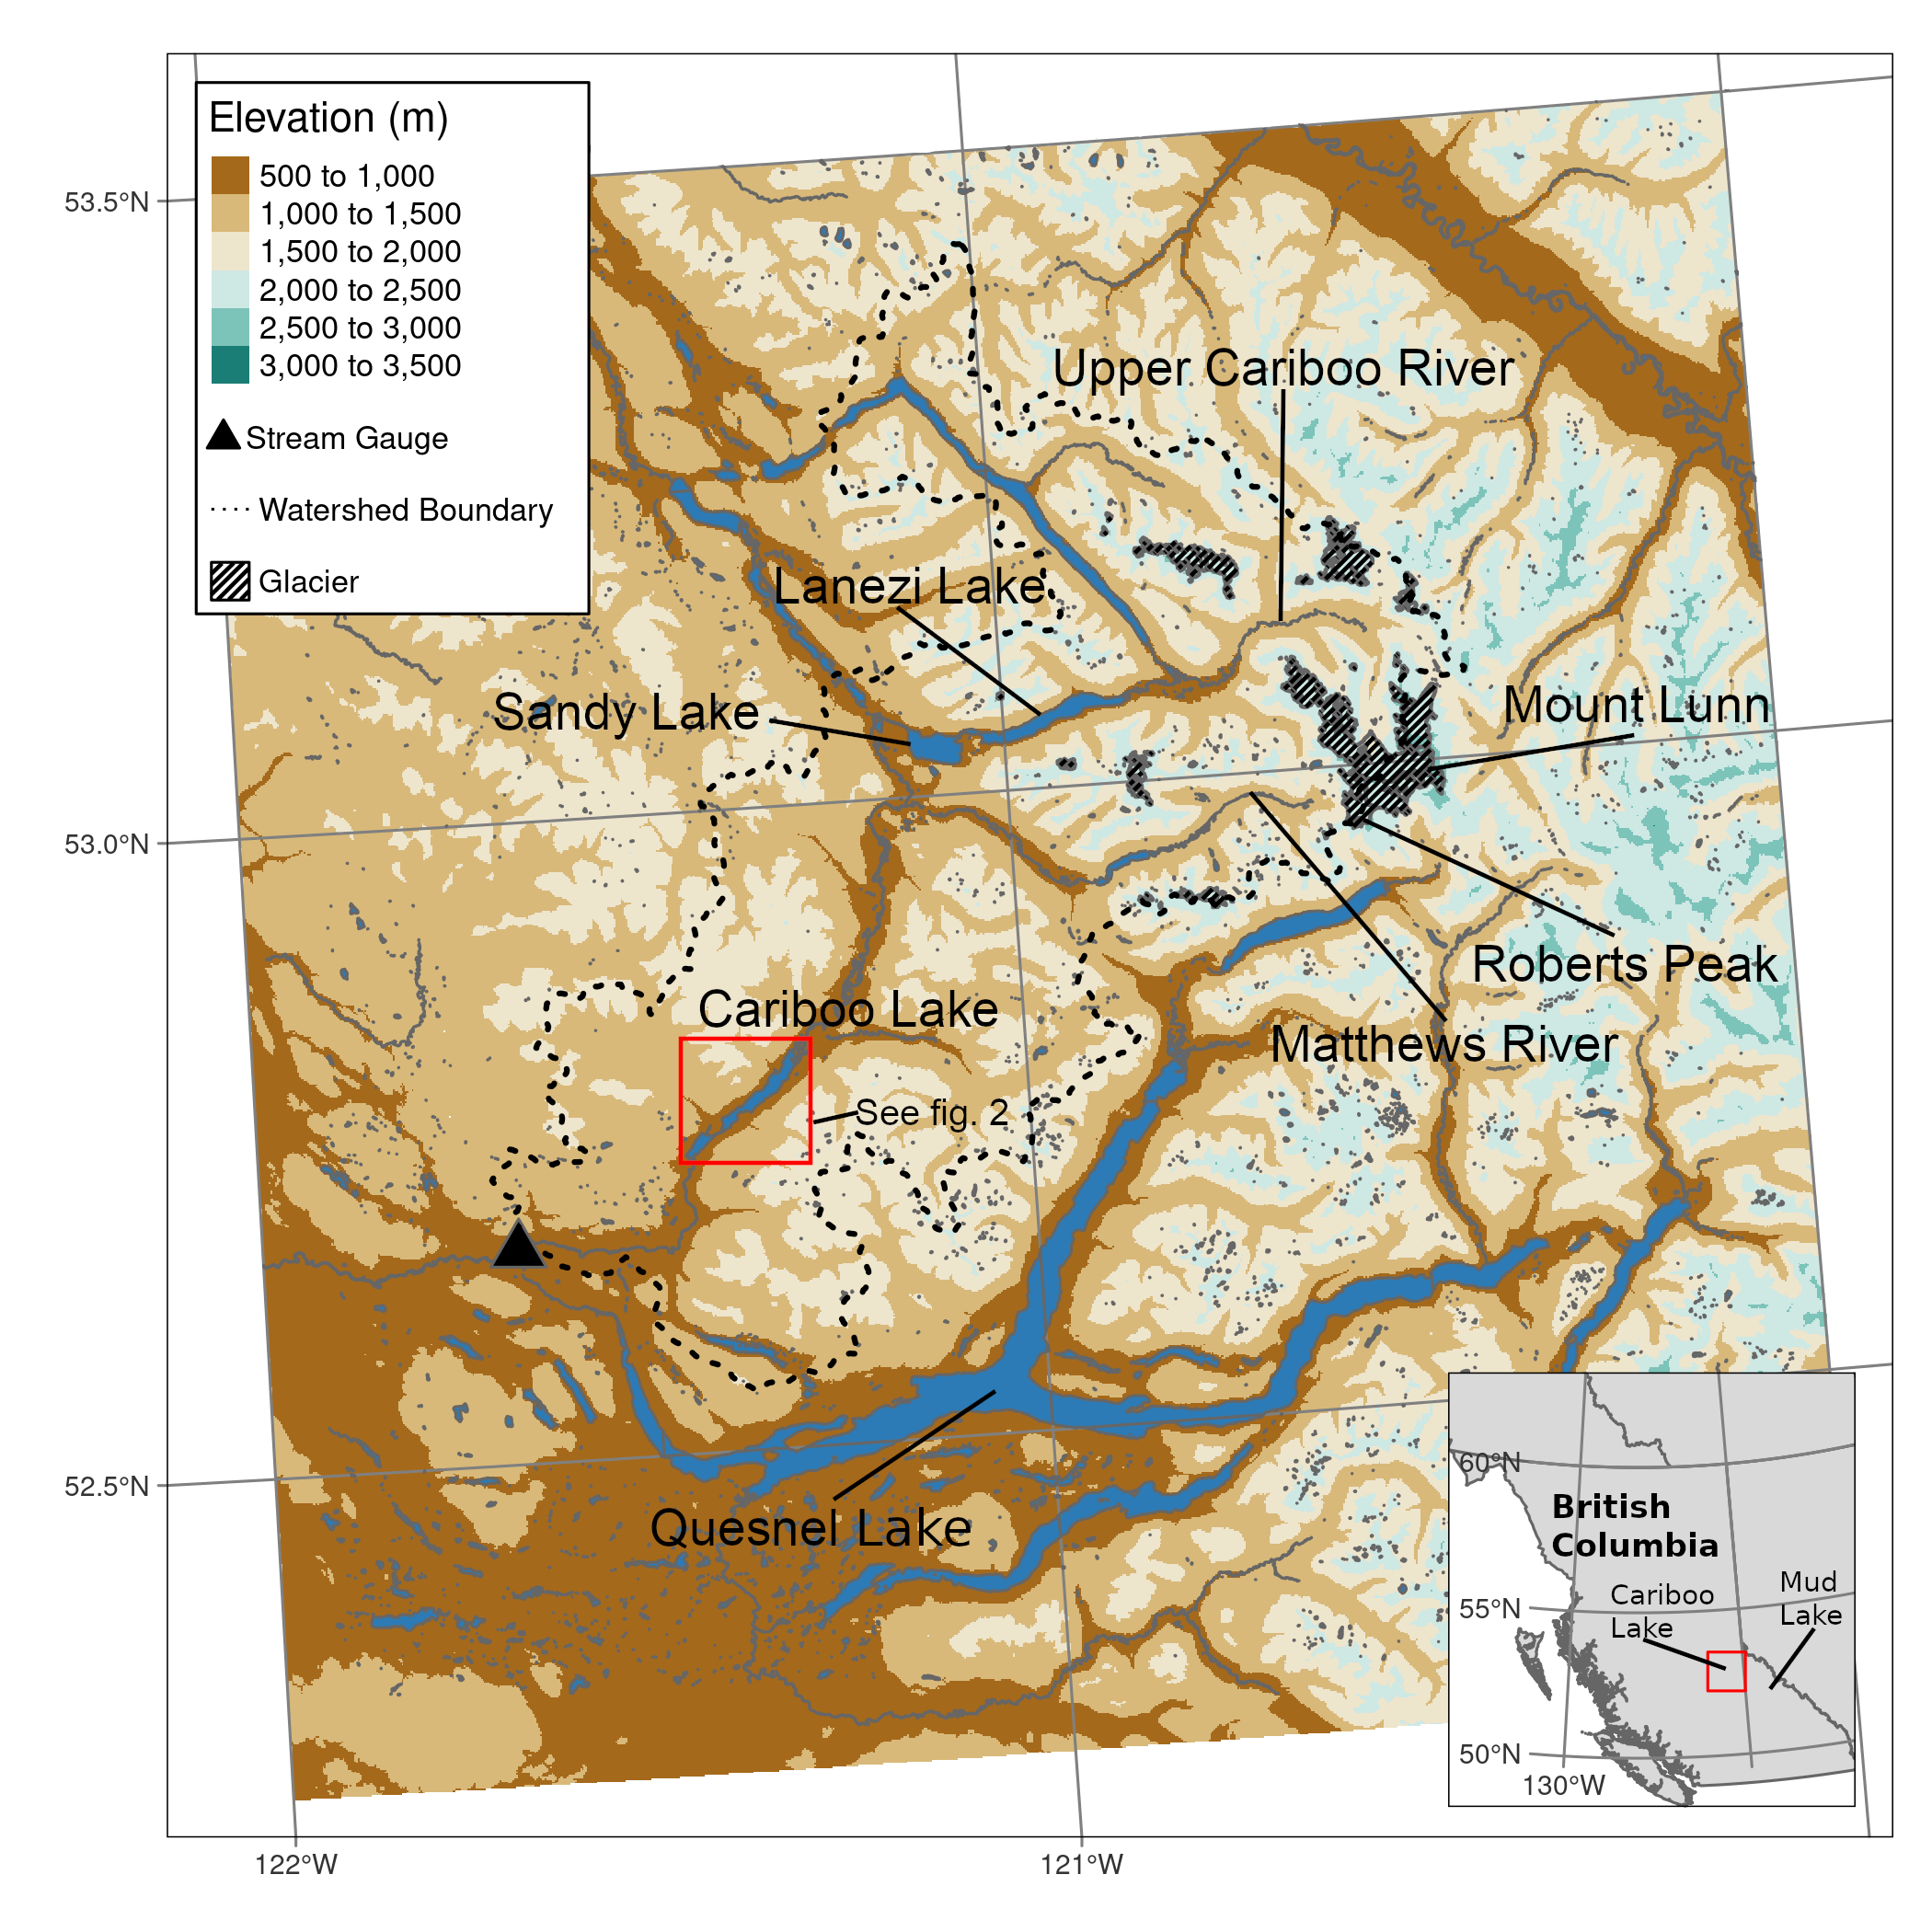
\includegraphics[width=1\linewidth]{figs/cl_small_scale_inset_labels_gimp} 

}

\caption{Map of the Cariboo Lake basin. Inset map shows the location of the Cariboo Lake basin within British Columbia relative to the Mud Lake basin from the Hodder et. al, (2006) study. See Figure 2 for detailed map of Cariboo Lake.}\label{fig:map-basin}
\end{figure}

\begin{figure}

{\centering 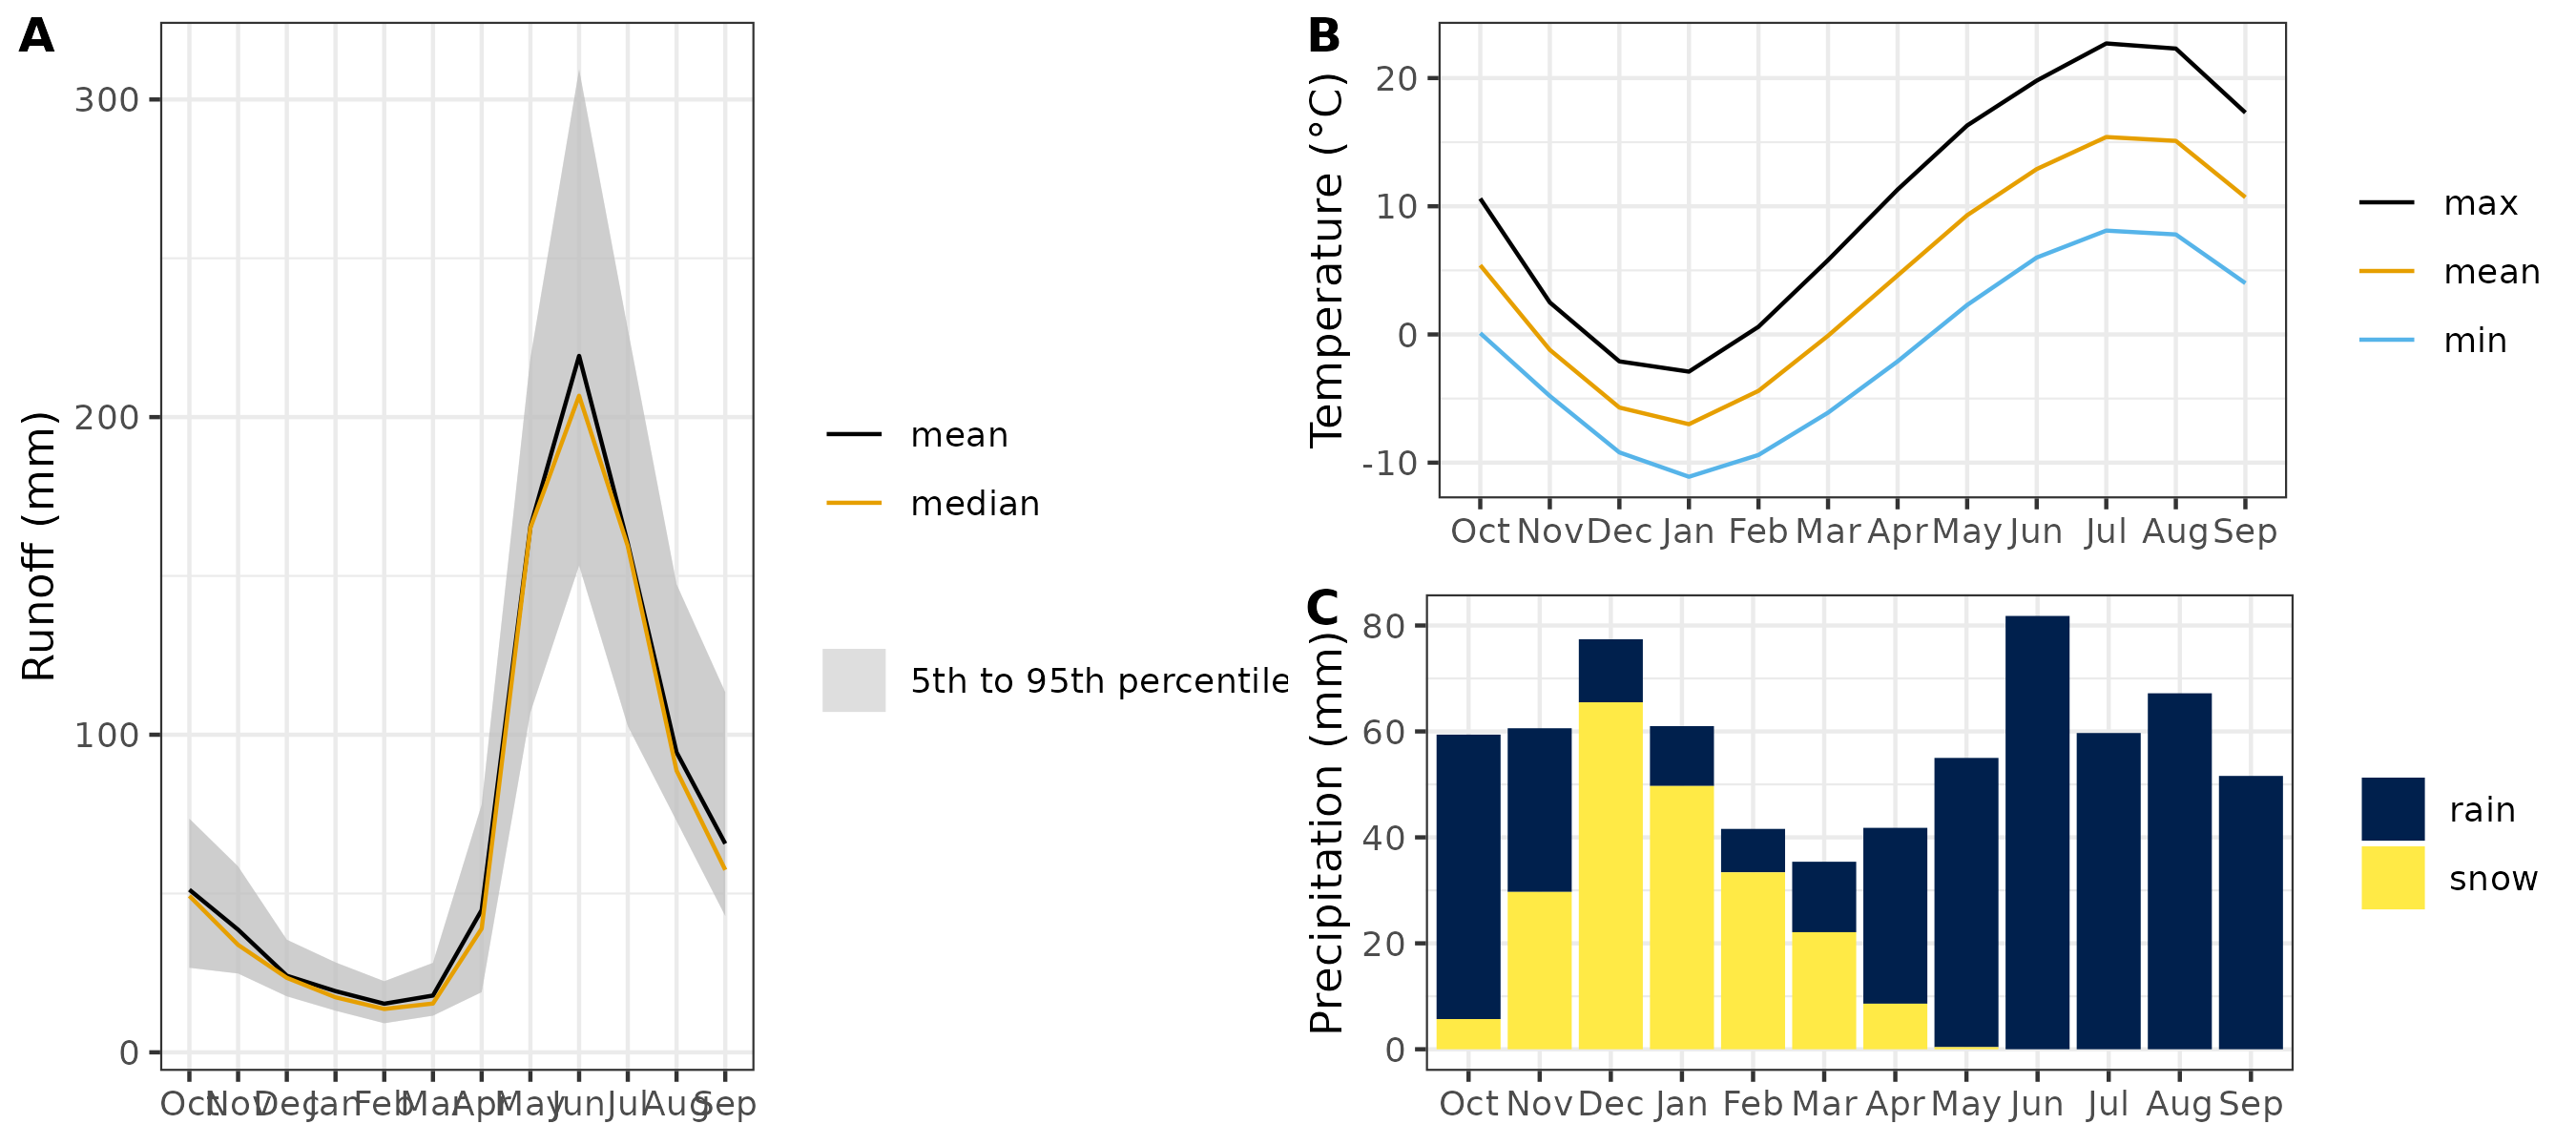
\includegraphics[width=1\linewidth]{figs/cariboo_combine_climate_hydro} 

}

\caption{1971-2000 monthly runoff statistics for Water Survey of Canada station 08KH003 (A) and 1971-2000 temperature and precipitation normals from Environment Canada station 1094616 (B). The top of each bar on panel C corresponds to the average monthly total precipitation and the coloured portion shows the fraction of rain or snow.}\label{fig:cl-hydro}
\end{figure}

\textbf{Lanezi Lake is a deep fjord-like lake with a flat lake bottom
bathymetry reaching a maximum depth of 170 m and suggests sediment
delivery to this lake has been relatively high over the Holocene (Figure
\ref{fig:map-basin}).} Sandy Lake is much shallower reaching a maximum
depth of 6 m. The Matthews River, which meets the Cariboo River just
below Lanezi Lake provides a less filtered connection to meltwater
sources draining several alpine glaciers including the largest area of
ice (10 km\textsuperscript{2}) in the Cariboo Lake watershed, proximal
to Roberts Peak (Figure \ref{fig:map-basin}).

\begin{figure}

{\centering \includegraphics[width=1\linewidth]{figs/cl_bathymetry_acoustics_coring_locations_labels} 

}

\caption{Map of the Cariboo Lake bathymetry and coring locations. Bathymetric interval is 10 m. Acoustic transects selected for analysis are shown with a black solid line and labeled A, B, C, D, E and F. Fan deltas mentioned in the text are represented by black triangles and are referenced to by the upstream creek (i.e. Frank Creek Delta is the triangle below Frank Creek). The Frank Creek fan delta separates the main Cariboo Lake and Frank Creek sub-basins. The Keithley Creek fan delta separates the Frank Creek and Keithley Creek sub-basins.}\label{fig:map-lake}
\end{figure}

\hypertarget{methods}{%
\section{Methods}\label{methods}}

\hypertarget{field-methods}{%
\subsection{Field Methods}\label{field-methods}}

A field campaign was conducted during the summer of 2017 to collect
sub-bottom acoustic soundings, dredge samples, and sediment cores.
Thirty-four km of sub-bottom acoustic soundings were collected across
Cariboo Lake using a 10 kHz StrataBox 3510 HD. An Ekman dredge was used
to collect 20 samples from the lake bottom, each yielding
\textasciitilde730 cm\textsuperscript{3} of surficial sediment. The
dredge samples were sub-sampled in the field using an 80 mm diameter PVC
cylinder pushed into the block of sediment. This resulted in 20 short
cores each containing about 450 cm\textsuperscript{3} of sediment.
\textbf{The Ekman dredge filled with variable depths of sediment and as
a result the short cores ranged from 6 to 12 cm in length.} The
remaining sediment not captured in the PVC cylinder was kept as a bulk
sediment sample. Four long sediment cores (V1-V4) were collected using a
Rossfelder submersible vibracorer with a 6 m long 70 mm diameter
aluminum pipe. The Ekman short cores and the long vibracores were split
longitudinally with one half preserved as an archive and the other as a
working half. The working half samples were prepared for imaging by
scraping the core parallel to the sediment laminae to create a flat
surface which showed the sediment stratigraphy. \textbf{The stratigraphy
of long cores V1 and V2 were selected for detailed analysis as they were
located within the deepest parts of upper Cariboo Lake. The deep
mid-lake sampling locations were important to ensure the cores consisted
of a higher fraction of fine clastic sediments from the main Cariboo
River compared to coarser sediments derrived from steep valley sidewalls
and turbidite flood events. Cores V3 and V4 taken at shallower depths
further down-lake had higher fractions of coarse grained sediments and
resulted in a higher degree of core disturbance, presumably due to the
lower cohesion of the coarser grained sediments.}

\hypertarget{laboratory-methods}{%
\subsection{Laboratory Methods}\label{laboratory-methods}}

The cores and short cores were analyzed for laminae thickness, organic
content, and particle size. The working halves of long cores V1 and V2
were subsampled with 2 cm\textsuperscript{3} of sediment extracted at a
5 cm interval, with additional samples taken within stratigraphic
breaks. Stratigraphic breaks were identified based on visual changes in
grain size and lamination patterns. Laminae couplets observed on the
\textbf{working halves} were digitally counted and measured for
thickness using the ImageJ software, by \citet{Schneider2012}.
\textbf{Uncertainty in laminae counting is attributed to sections of
core with indiscernible laminae formation, core compaction,
undercounting, and subjectivity in classifying the occasionally thicker
(4 to 47 mm thick) graded to massive laminae/beds. Varve counting
uncertainties in the literature are reported as ranging between 0.7 - 6
\% \citep{Menounos2008c, Zolitschka1991}. The uncertainty of the laminae
counting in this study was inferred from Ekman short cores (E12, E13,
E14) which had statistically similar sediment accumulation rates. The
varve counting error was estimated by counting the number of couplets
down to a specific depth of 5 cm in each Ekman core resulting in a
standard deviation between the counts for each core.} The top section of
cores V1 and V2 were disturbed during coring - 110 mm for V1 and 70 mm
for V2 which prevented counting and measurement of laminae couplets.
Organic content was determined by loss-on-ignition analysis (550 °C)
following methods in \citet{Smith2003}. Samples were first weighed to
provide an initial wet weight, then dried at 60 °C and weighed again
after oven drying. The samples were then placed in a furnace at 550 °C
for 2.5 hours and weighed a third time. Grain size analysis was
conducted using a Mastersizer Particle Size Analyzer 3000. Samples were
prepared following methods by \citet{Gray2010} to remove the fine
fraction of particles from organic material. This involved a removal of
organic material using three sequential alloquots of 20\%
H\textsubscript{2}0\textsubscript{2} until the sample stopped reacting.
To prevent flocculation of sediment grains the samples were dispersed in
0.05\% solution of Calgon for 24 hours. Grain size was measured three
times for each sample, resulting in an average standard deviation of ±
0.01 µm. The chronology of both vibra cores was reconstructed using AMS
\textsuperscript{14}C dating (analyzed at the André E. Lalonde AMS
Laboratory at the University of Ottawa) and a chronology derived from
laminae (couplet) counting on working core images. The AMS
\textsuperscript{14}C calibration was performed using Bchron, a
Baysesian statistical age-model software package for R
\citep{Parnell2008, Parnell2011, Haslett2008} and the IntCal13
calibration curve \citep{Reimer2013}.

\hypertarget{results}{%
\section{Results}\label{results}}

\hypertarget{sub-bottom-acoustics}{%
\subsection{Sub-bottom Acoustics}\label{sub-bottom-acoustics}}

Acoustic stratigraphy from six selected transects (see locations in
Figure \ref{fig:map-lake}) reveal the range of morphologies and
character of sedimentary deposits in Cariboo Lake (Figure
\ref{fig:acoustics}). Acoustic penetration is limited in transects A and
E by coarser sediments proximal to river fan-deltas across Cariboo Lake
(see triangle symbols in Figure \ref{fig:map-lake} for fan-delta
locations). Acoustic signal penetration, resolution and distinctive
acoustic layering improves significantly along the thalweg of the lake
bottom away from the main Cariboo River delta and in cross-lake
transects more distal from the valley-side fan-deltas. \textbf{The
diagnal lines across all panels (cross-hatching) in Figure
\ref{fig:acoustics} is observed over most of the acoustic record due to
errant electrical interference from the research vessel that could not
be resolved.} However, the interference does not affect the overall
quality of the acoustic results in the six selected transects (Figure
\ref{fig:acoustics}, A-F).

Transect A, one kilometer southwest of the headwater Cariboo River
delta, has a strong acoustic reflector at the sediment-water interface
indicating the presence of coarser-grained material on the lakebed
(Figure \ref{fig:acoustics}, A). Grab samples on this transect show a
high fraction of sandy materials which act as an acoustic mask limiting
the penetration of the acoustic signal to a depth of 1-2 m. An acoustic
multiple (echo) is observed 45 m below the sediment surface caused by
the limited penetration at the surface (Figure \ref{fig:acoustics}, A -
i). Acoustically penetrable, well-layered sediment is observed 3.5 km
from the Cariboo River delta in transect B (Figure \ref{fig:acoustics},
B). This site is proximal to long core V1. Acoustic reflectors with 1-2
m separation lie conformably over a hummocky basement which is observed
on the south side of the transect (Figure \ref{fig:acoustics}, B - i).
The acoustic basement drops off below the observable record near the
south channel-like depression. Well structured layering extends across
the south side of the transect but pinches out towards the north shore
(Figure \ref{fig:acoustics}, B, C \& D). On the south side of transect
B, the thickness of the well structured layering ranges from 10 to 20 m.
Underlying the layered sediments is a more massively layered facies
which ranges from 12 to 25 m thick before the record is cut off below
the maximum depth of the record of 80 m.

\begin{figure}

{\centering 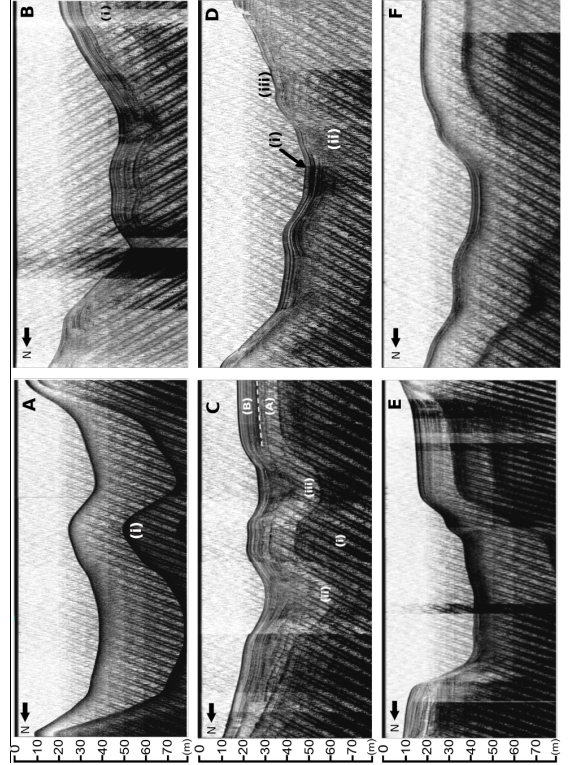
\includegraphics[width=1\linewidth]{figs/acoustics_6_panel} 

}

\caption{Panel of six selected sub-bottom acoustic transects A, B, C, D, E, and F. The left-hand side of each transect corresponds to the north-shore of the lake, see Figure 2 for location of each transect. Transect A and B: Acoustic echo (multiple) is denoted by (i). Transect C: (i) denotes inferred bedrock or coarse late-glacial material. (ii) and (iii) are v-notch scour channels. (A) and (B) are sediment facies. Transect D: Scour channels are denoted by (i) and (ii). Slumping is observed at (iii).}\label{fig:acoustics}
\end{figure}

Acoustic penetration increases 4.5 km from the Cariboo River delta at
transect C (Figure \ref{fig:acoustics}, C). The acoustic record along
this transect reaches a maximum sediment thickness of 35 m in two
troughs, the maximum thickness of surficial sediments observed across
Cariboo Lake in this study. The acoustic basement is considered to be
either bedrock or coarse-grained glacial sediment from the Last Glacial
Maximum (Figure \ref{fig:acoustics}, C -- i). Two sediment facies are
observed across this transect based on geometry and the strength and
continuity of reflectors. Some disruption of these facies is caused by
slumping of side slopes (e.g.~north end of transect C). The lower unit,
facies A, has a thickness of \textasciitilde12 m along undisturbed
sections (Figure \ref{fig:acoustics}, C) and is more massive to weakly
acoustically layered. The contact with overlying sediment above facies A
appears to be conformable at the south end and middle of the transect
but unconformable in other places. The unconformities are most apparent
in the two sharp crested v-notch channels at the middle of the transect.
These channels are a continuation of those noted in transect B. These
are inferred to be scour channels formed by erosive, higher energy,
turbidity currents that probably date to deglaciation of the lake basin.
The lack of numerous layers and generally lighter grey tone in facies A
indicates a somewhat higher energy and more rapid deposition of coarser
lacustrine sediment. Facies B begins with high-amplitude parallel
reflectors with 2-3 m separation and conforms well with facies A below
(Figure \ref{fig:acoustics}, C). Facies B has a thickness of
\textasciitilde10 m along undisturbed sections and deepens to a maximum
of 13 m within the scour channels (Figure \ref{fig:acoustics}, C - ii \&
iii). The strength of reflectors in facies B are stronger and more
numerous than those in facies A indicating more frequent events of lower
overall magnitude during this time. The strength of reflectors gradually
decreases moving upwards and spacing thins to sub metre thickness near
the surface. The gradual decrease in reflectance is interrupted by a
strong reflector at the top of facies B along the sediment-water
interface.

The two buried troughs in transect C (Figure \ref{fig:acoustics}, C -
ii, iii) are significant and best expressed in this area of the lake.
The north trough (ii) appears to be a depression that was continuously
infilled by facies A and then B. Hence it most likely represents an
older pre-existing feature. The sediments in the southern trough (iii)
are interesting in that a wedge of sediment infill seems to be an
unconformable deposit with both facies B below and facies A above. This
wedge of sediment is observed in Figure \ref{fig:acoustics} above label
C-iii characterized by a deepening of facies B and darker in color than
facies A. It is likely that an erosional channel developed after or in
the later stages of facies A deposition which infilled the wedge.
Sedimentation of the wedge was then truncated by the onset of the facies
B sediment. While the two troughs might have been active at the same
time during deglaciation, only the southern trough was reactivated at a
later time and infilled with sediment prior to the onset of facies B
deposition.

Transect D, to the northeast of the Frank Creek delta has well-layered
sediments in the top 5-10 m and transitions to poor acoustic penetration
below this (Figure \ref{fig:acoustics}, D). The parallel reflectors
observed in the uppermost sediment layers of transect D have a thickness
of 2-3 m and have a higher amplitude compared to facies B in transect C.
Some slumping of sidewall sediments is observed on the south sidewall
(Figure \ref{fig:acoustics}, D).

Southwest of the Frank Creek fan-delta, acoustic reflectors along
transect E show a decline in reflectance and a decrease in layer
thickness to \textless{} 1 m. Acoustic masking from coarse grained
sediment occurs at depths of 2-4 m along the south margin (Figure
\ref{fig:acoustics}, E). Total sediment thickness of finer, acoustically
well-layered material along the north bench is significant approaching
10 m. The profile suggests that much of the suspended sediment
transported from the upper lake does not make it past the shallow lake
depths (\textless{} 20 m) of the sill at the Frank Creek fan-delta apart
from the northern most part of the transect. Coarser sediment from the
Frank Creek fan-delta dominates the south side of the transect and fine
sediment deposition is restricted, or forced, to the north side.

Similar to the Frank Creek fan-delta, the very shallow sill of less than
2 m opposite the Keithley Creek prograding fan-delta significantly
reduces sediment connectivity to the main Cariboo Lake basin (see
triangle proximal to Keithley Creek in Figure \ref{fig:map-lake}).
Transect F, located close to the centre of the Keithley Creek sub-basin
shows a maximum observable sediment thickness of 4 m concentrated in the
basin thalweg (Figure \ref{fig:acoustics}). Below this there is acoustic
masking by coarser sediment. The acoustic reflectors within the top 4 m
of transect F are acoustically penetrable, well layered and are
conformable to the basin morphology. These reflectors are of higher
amplitude compared to those in transect E and are thicker at 1-2 m. This
suggests that significant amounts of coarse-grained sediments are found
in this part of the lake, likely originating from the high energy
Keithley Creek drainage basin. Fine faction sediments from the main
Cariboo Lake are expected to make up a small percentage as transport
into this sub-basin is limited by up-lake storage, filtering and
hypopycnal overpassing.

\hypertarget{spatial}{%
\subsection{Spatial Trends in Surficial Sediment}\label{spatial}}

Twenty surficial sediment cores ranging from 6-12 cm thick were analyzed
for grain size, laminae thickness, and organic content. These samples
were collected following a longitudinal transect down Cariboo Lake and
indicate how sediment flux varies with distance from the Cariboo River
delta (see Figure \ref{fig:map-lake}, for sampling locations).
\textbf{The percent of sand-sized sediments follows an exponential
decline with distance down-lake starting at 60.8 \% sand proximal to the
Cariboo River delta and reaching a low of 0.15 \%, 5.2 km km from the
Cariboo River delta (Figure \ref{fig:ekmanSeds}, A). The
D\textsubscript{50} grain size also follows a steep decline from 89.9
µm, 300 m from the delta, to 31.3 µm 550 m from the Cariboo River delta
(Figure \ref{fig:ekmanSeds}, B). The decline in D\textsubscript{90}
grain size follows a more pronounced decline, while the
D\textsubscript{10} remains largely unchanged. This suggests that larger
sand-sized sediments (63-2000 µm) are sensitive to distance from fan
deltas, while smaller silt-sized (2-63 µm) and clay-sized (0.01-2 µm)
sediments are less sensitive. At distances greater than 2 km from the
Cariboo River delta the fraction of silt-sized sediments remains at over
80 \%, aside from core E16 which is near the Frank Creek fan-delta. The
highest percent of silt (86.5-89.6 \%) and clay (9.3-14.4 \%) sized
sediments are observed between 3 and 6.5 km from the Cariboo River
delta, proximal to the long core sampling locations.} Near to the Frank
Creek fan-delta the D\textsubscript{50} grain size nearly doubles in
size from 7.92 µm at 6.4 km to 15.1 µm at 7.35 km from the Cariboo River
delta. In the Keithley Creek sub-basin the D\textsubscript{50} grain
size has an average grain size of 15.9 µm (n = 3) and the composition of
sediment is 4.0\% clay, 85.8\% silt, and 10.2\% sand (Figure
\ref{fig:ekmanSeds}, A, B).

Proximal to the Cariboo River delta (\textless{} 500 m) the structure of
the surficial sediments exhibits massive layering, erosive contacts and
the fraction of sand grains in these samples is greater than 60\%. A
sand-bed with a thickness of 1 cm is observed in the bulk sample closest
to the Cariboo River delta (Figure \ref{fig:ekmanImgs}, A). In the main
Cariboo River basin, core E13 had the most distinct laminations and was
taken 5.24 km from the Cariboo River delta, proximal to long core V2, in
the deepest part at a depth of 40 m. Sediment here shows rhythmic
lamination (Figure \ref{fig:ekmanImgs}, B).

\begin{figure}

{\centering 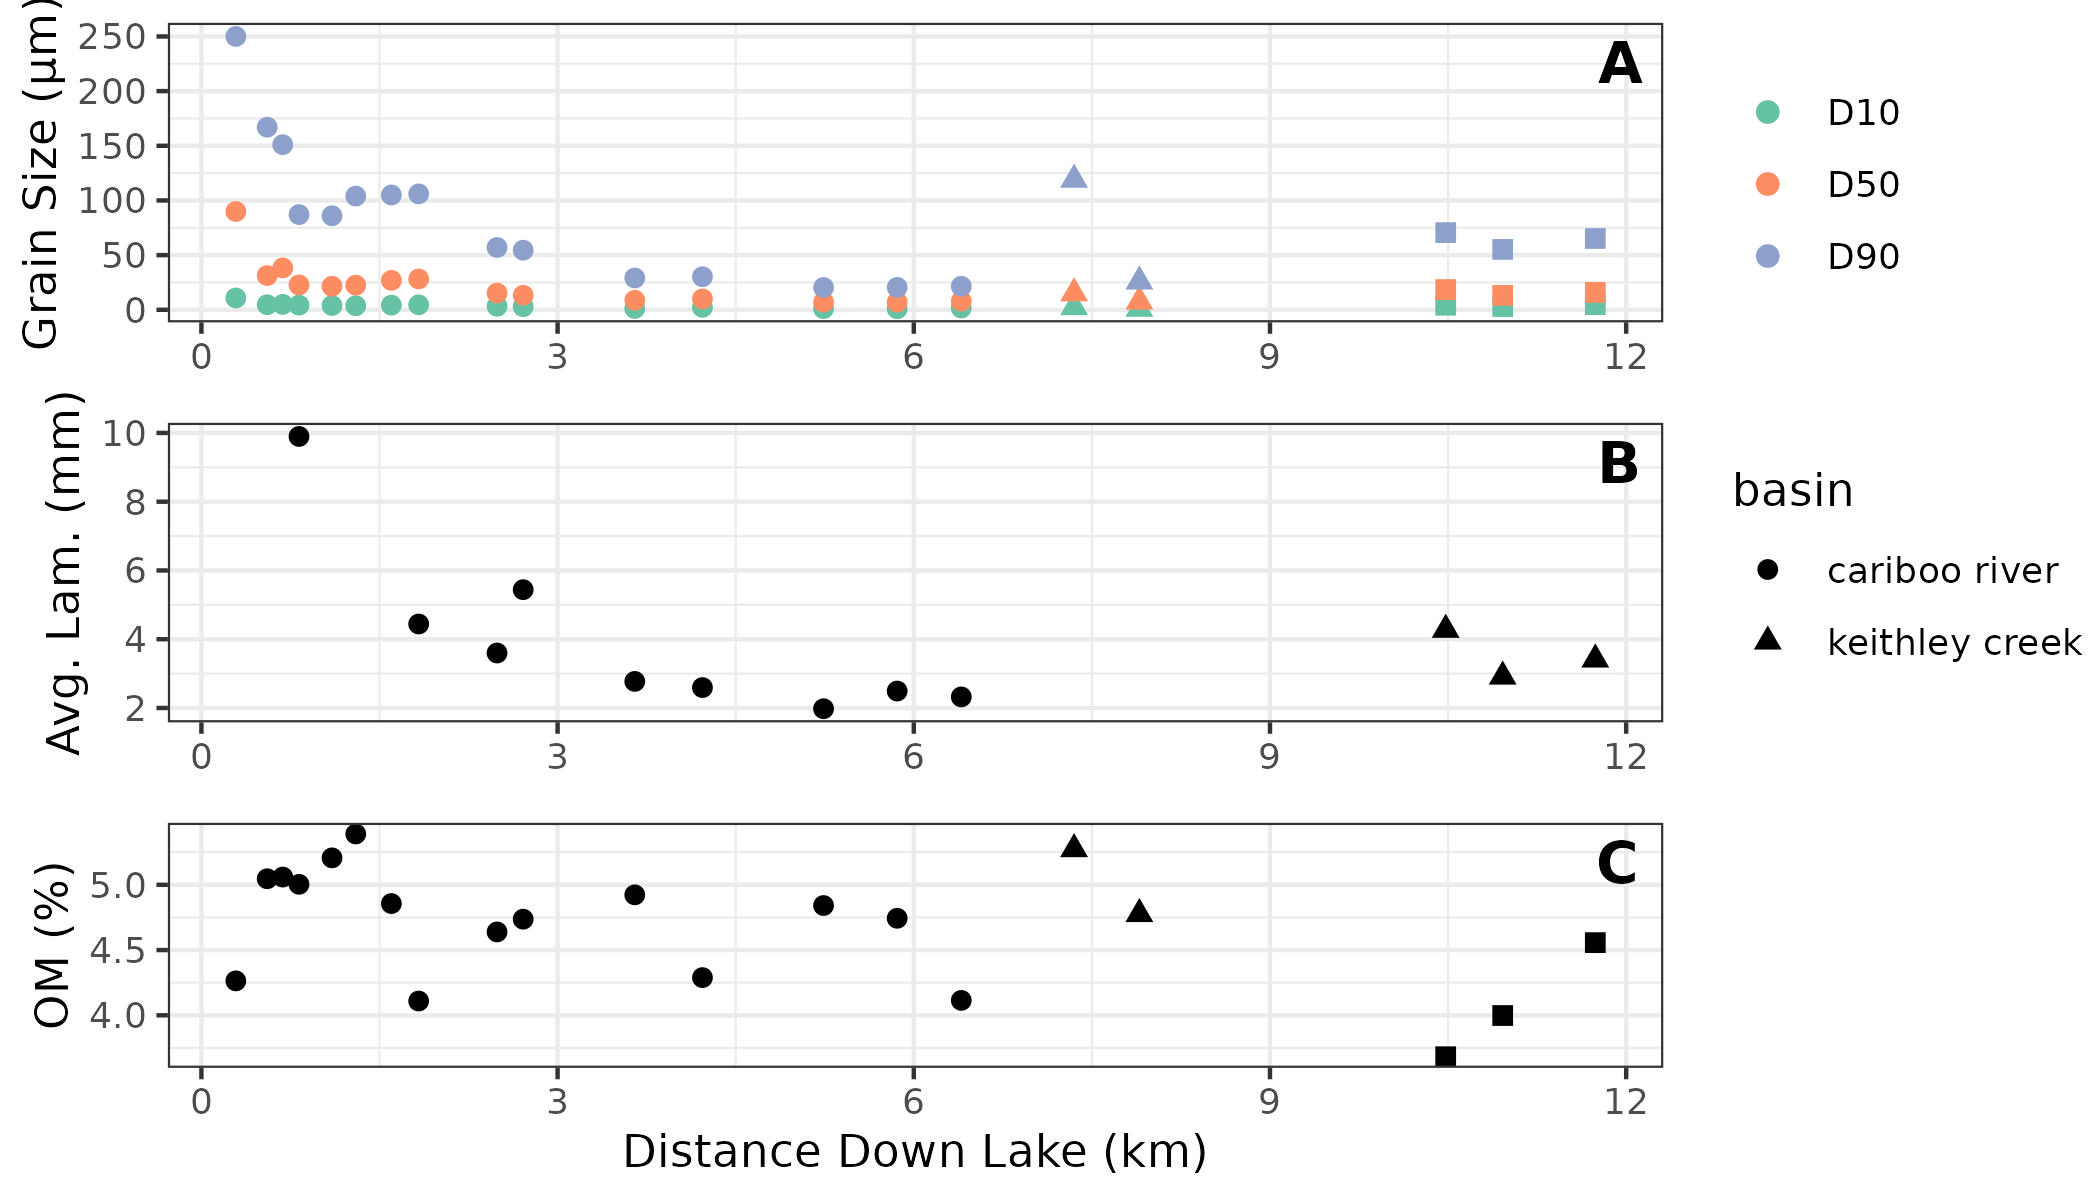
\includegraphics[width=1\linewidth]{figs/ekman_seds} 

}

\caption{Sediment characteristics from the Ekman surficial bulk samples with distance down lake from the Cariboo River input to Cariboo Lake. Top panel A is the percent clay (0.01 - 2) µm, silt (2 - 63) µm, and sand grains (63 - 2000) µm, panel B is the  D~10~, D~50~, and D~90~ (µm) grain size, panel C is the mean laminae thickness (mm), and the bottom panel D is percent organic matter content (OM).}\label{fig:ekmanSeds}
\end{figure}

\begin{figure}

{\centering 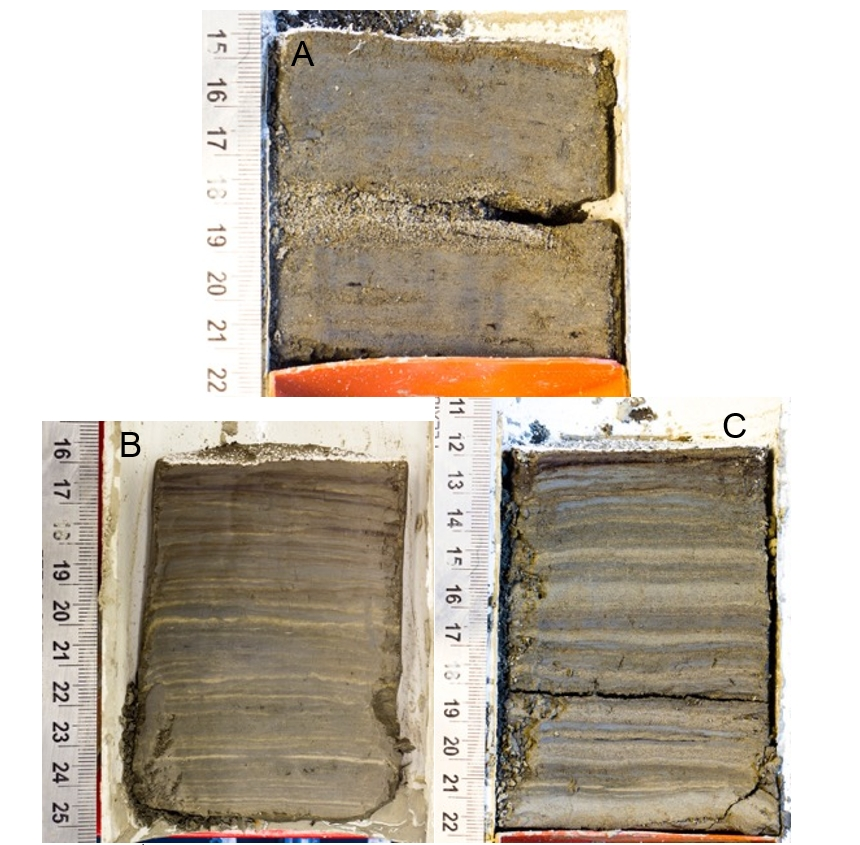
\includegraphics[width=1\linewidth]{figs/ekman_example} 

}

\caption{Selected surficial Ekman sediment core photographs. A (E1) is proximal to the Cariboo River delta (0.3 km down lake). B (E13) was retrieved from the second deepest basin in the lake in the Cariboo River basin (5.24 km down lake). C (E18) was retrieved from the Keithley Creek sub-basin (29.53 km down lake).}\label{fig:ekmanImgs}
\end{figure}

Sediment cores E9-E15 and E18-E20, retrieved from areas in Cariboo Lake
that are distal from river deltas and have lake depths of 30-50 m, have
a high fraction of silt and clay sediment and exhibit a sequence of
fine-grained dark layers followed by coarse-grained light layers (Figure
\ref{fig:ekmanImgs}, B \& C). \textbf{The sediment stratigraphy observed
within cores E9-E15 and E18-E20 is similar to annual laminations (also
called varves) observed in many other lakes
\citep{Cockburn2008, Zolitschka2015a, Heideman2015, Hodder2006b, Desloges1999}
that have sufficient seasonal variation in river discharge and lake
stratification. In the Cariboo Lake basin, winter low flows, lake-ice
cover, and lake stratification reduce the velocity of lake currents and
contribute to the deposition of fine-grained sediments on the lake
bottom. During the spring nival high flows, coarser-grained sediments
are deposited as a result of higher energy lake currents. Additional
deposits of coarse-grained sediment also may result due to abnormally
high discharge events such as large rain or snow-melt events and/or
turbidite beds due to delta collapse \citep{sabatier2022}. Coastal lakes
in western Canada that are frequented by large rain storms and
mid-winter melt events lead to multiple laminae couplets deposited in a
given year \citep{Menounos2008c}. However, the distinct spring
snowmelt-dominant hydrological regime of the Cariboo Lake watershed
shown in Figure \ref{fig:cl-hydro} suggests the deposit of multiple
coarse-grained laminae in one year is rare. Coarse-grained deposits are
still possible in Cariboo Lake due to turbidite beds from delta
slumping/foreset failures however these turbidite beds are only observed
in Ekman cores proximal to Cariboo Lake river deltas
(e.g.~\ref{fig:ekmanImgs}, A). While the sediment stratigraphy of Ekman
cores E9-E15 and E18-E20 resemble varves, further analysis of the
Cariboo Lake long-cores and C14 chronology is required to confirm this.}

The thickness of sediment laminae couplets within cores E9-E15 and
E18-E20 demonstrate a gradual decreasing trend with distance down-lake
from the Cariboo River delta (Figure \ref{fig:ekmanSeds}, B). This
suggests the Cariboo River is the main source of sediment into Cariboo
Lake as sediment flux typically declines with distance from the primary
sediment source. Maximum couplet thickness has an average of 4.7 mm (n =
6) in the Cariboo River basin and 7.9 mm (n = 3) in the Keithley Creek
sub-basin. In the Cariboo River basin, maximum couplet thickness
decreases by 0.62 mm/km and by 2.17 mm/km in the Keithley Creek
sub-basin with distance down-lake (Figure \ref{fig:ekmanSeds}, B). The
decline in thickness is more rapid in the Keithley Creek sub-basin is
likely due to additional local inputs of coarser grained sediment coming
from the Keithley Creek tributary.

Trends in percent organic matter (OM) of surficial sediment cores were
not found to exhibit systematic patterns with distance down-lake (Figure
\ref{fig:ekmanSeds}, C). \textbf{The lowest OM values were observed in
the Keithley Creek sub-basin and suggest higher levels of clastic
sediment yield in this basin which dilutes the OM signal.}

The results from particle size, laminae thickness, and percent organics
\textbf{supports the hypothesis that} sediment delivered from the main
Cariboo River is the primary source of sediment to Cariboo Lake. Massive
layering of sediment and coarse-grained particle sizes are limited to
areas proximal to Pine Creek, Frank Creek and Keithley Creek deltas
where localized turbidity currents are active. Outside of these areas,
where turbidity currents and bedload transport processes are reduced,
the sediment in Cariboo Lake is largely comprised of rhythmically
laminated silt and clay sediments likely transported primarily through
suspended sediment processes from the main Cariboo River. In the
Keithley Creek sub-basin grain size and laminae structures are larger in
size than those observed in the main Cariboo River basin suggesting
local sediment inputs from the Keithley Creek are significant (Figure
\ref{fig:ekmanImgs}, C).

\hypertarget{sediment-accumulation-chronology}{%
\subsection{Sediment Accumulation
Chronology}\label{sediment-accumulation-chronology}}

Four vibra sediment cores, ranging from 2 -- 4 m in length, were
retrieved from the deepest portions of Cariboo Lake (Figure
\ref{fig:map-lake}). Cores V1 (3 m) and V2 (4 m) in the main Cariboo
River basin were selected for detailed analysis as these two cores had
organic material for AMS radiocarbon dating, and their sediment
stratigraphy was well preserved. The chronology of the two cores is
provided by a small number of AMS radiocarbon dates and laminae
counting. \textbf{A search for volcanic tephra was made through careful
magnified inspection of visual color changes. None were found using this
method. \citet{Westgate1977}, \citet{Hallett1997} and
\citet{Maurer2012b} indicate that this area of British Columbia has had
episodic volcanic ash inputs from significant eruptions that predate
2100 years BP but nothing since. The chronology of the Cariboo lake core
records of grain size, varve thickness, and organic content demonstrate
patterns in sediment delivery to Cariboo Lake over approximately the
past 2000 years.}

\hypertarget{chronology}{%
\subsubsection{Chronology}\label{chronology}}

Organic material for dating in the clastic dominated cores was extremely
limited. AMS radiocarbon dates obtained for cores V1 and V2 are
presented in Table \ref{tab:amsDates} and provide limited temporal
control and evidence of sediment accumulation rates for the long cores.
A small twig from V1 at 343 cm and combination of two separate organic
pieces which were combined into one sample at V2, with an average depth
of 281 cm, yielding a calibrated \citep{Reimer2013} two-sigma date range
of 1820-1918 cal BP and 1895-2043 cal BP respectively. Figure
\ref{fig:amsRates} shows the \textsuperscript{14}C chronology for V1 and
V2 compared to the laminae couplet chronologies for E13, V1, and V2. The
\textsuperscript{14}C dates from samples V1 and V2 yield accumulation
rates \textbf{(depth of sample divided by age of sample)} of 1.76 ± 0.05
mm yr\textsuperscript{-1} and 1.37 ± 0.05 mm yr\textsuperscript{-1}
respectively.

\begin{longtable}[]{@{}
  >{\raggedright\arraybackslash}p{(\columnwidth - 12\tabcolsep) * \real{0.0926}}
  >{\raggedright\arraybackslash}p{(\columnwidth - 12\tabcolsep) * \real{0.0741}}
  >{\raggedright\arraybackslash}p{(\columnwidth - 12\tabcolsep) * \real{0.1019}}
  >{\raggedright\arraybackslash}p{(\columnwidth - 12\tabcolsep) * \real{0.1296}}
  >{\raggedright\arraybackslash}p{(\columnwidth - 12\tabcolsep) * \real{0.1481}}
  >{\raggedright\arraybackslash}p{(\columnwidth - 12\tabcolsep) * \real{0.2685}}
  >{\raggedright\arraybackslash}p{(\columnwidth - 12\tabcolsep) * \real{0.1852}}@{}}
\caption{Cariboo Lake chronologic control
points.\label{tab:amsDates}}\tabularnewline
\toprule()
\begin{minipage}[b]{\linewidth}\raggedright
Core Name
\end{minipage} & \begin{minipage}[b]{\linewidth}\raggedright
Type
\end{minipage} & \begin{minipage}[b]{\linewidth}\raggedright
Depth (cm)
\end{minipage} & \begin{minipage}[b]{\linewidth}\raggedright
\textsuperscript{14}C (yr BP)
\end{minipage} & \begin{minipage}[b]{\linewidth}\raggedright
\textsuperscript{14}C 1\(\sigma\)
\end{minipage} & \begin{minipage}[b]{\linewidth}\raggedright
2\(\sigma\) age range (cal BP)
\end{minipage} & \begin{minipage}[b]{\linewidth}\raggedright
Median age (cal BP)
\end{minipage} \\
\midrule()
\endfirsthead
\toprule()
\begin{minipage}[b]{\linewidth}\raggedright
Core Name
\end{minipage} & \begin{minipage}[b]{\linewidth}\raggedright
Type
\end{minipage} & \begin{minipage}[b]{\linewidth}\raggedright
Depth (cm)
\end{minipage} & \begin{minipage}[b]{\linewidth}\raggedright
\textsuperscript{14}C (yr BP)
\end{minipage} & \begin{minipage}[b]{\linewidth}\raggedright
\textsuperscript{14}C 1\(\sigma\)
\end{minipage} & \begin{minipage}[b]{\linewidth}\raggedright
2\(\sigma\) age range (cal BP)
\end{minipage} & \begin{minipage}[b]{\linewidth}\raggedright
Median age (cal BP)
\end{minipage} \\
\midrule()
\endhead
V1 & Surface & NA & NA & NA & NA & NA \\
V1 & 14C & NA & 1913 & 21 & 1820-1918 & NA \\
V2 & Surface & NA & NA & NA & NA & NA \\
V2 & 14C & NA & 2020 & 28 & 1895-2043 & NA \\
\bottomrule()
\end{longtable}

Ekman surficial core 13 (E13), shown in Figure \ref{fig:amsRates}, is
most proximal to the V2 long core (see Figure \ref{fig:map-lake}) and
exhibits similar sediment accumulation compared to the
\textsuperscript{14}C and laminae chronology of V2. The light-dark
couplets in E13, shown in Figure \ref{fig:ekmanImgs}, are similar to
annual deposits noted in dozens of other lakes throughout BC
\citep[e.g.][]{Hodder2006b}. Therefore, the couplets within the Ekman
cores are assumed to closely approximate varves, in which case E13
exhibits an average accumulation rate of 1.98 ± 0.19 mm
yr\textsuperscript{-1}. Higher accumulation rates are expected for the
Ekman samples as they are not subjected to the same level of compaction
as is deeper sediment in the long cores. The consistency of the E13
inferred accumulation rate when compared with two of the AMS dates from
the V1 and V2 cores (Figure \ref{fig:amsRates}) are additional evidence
of the varved nature of the sediment record.

\begin{figure}

{\centering 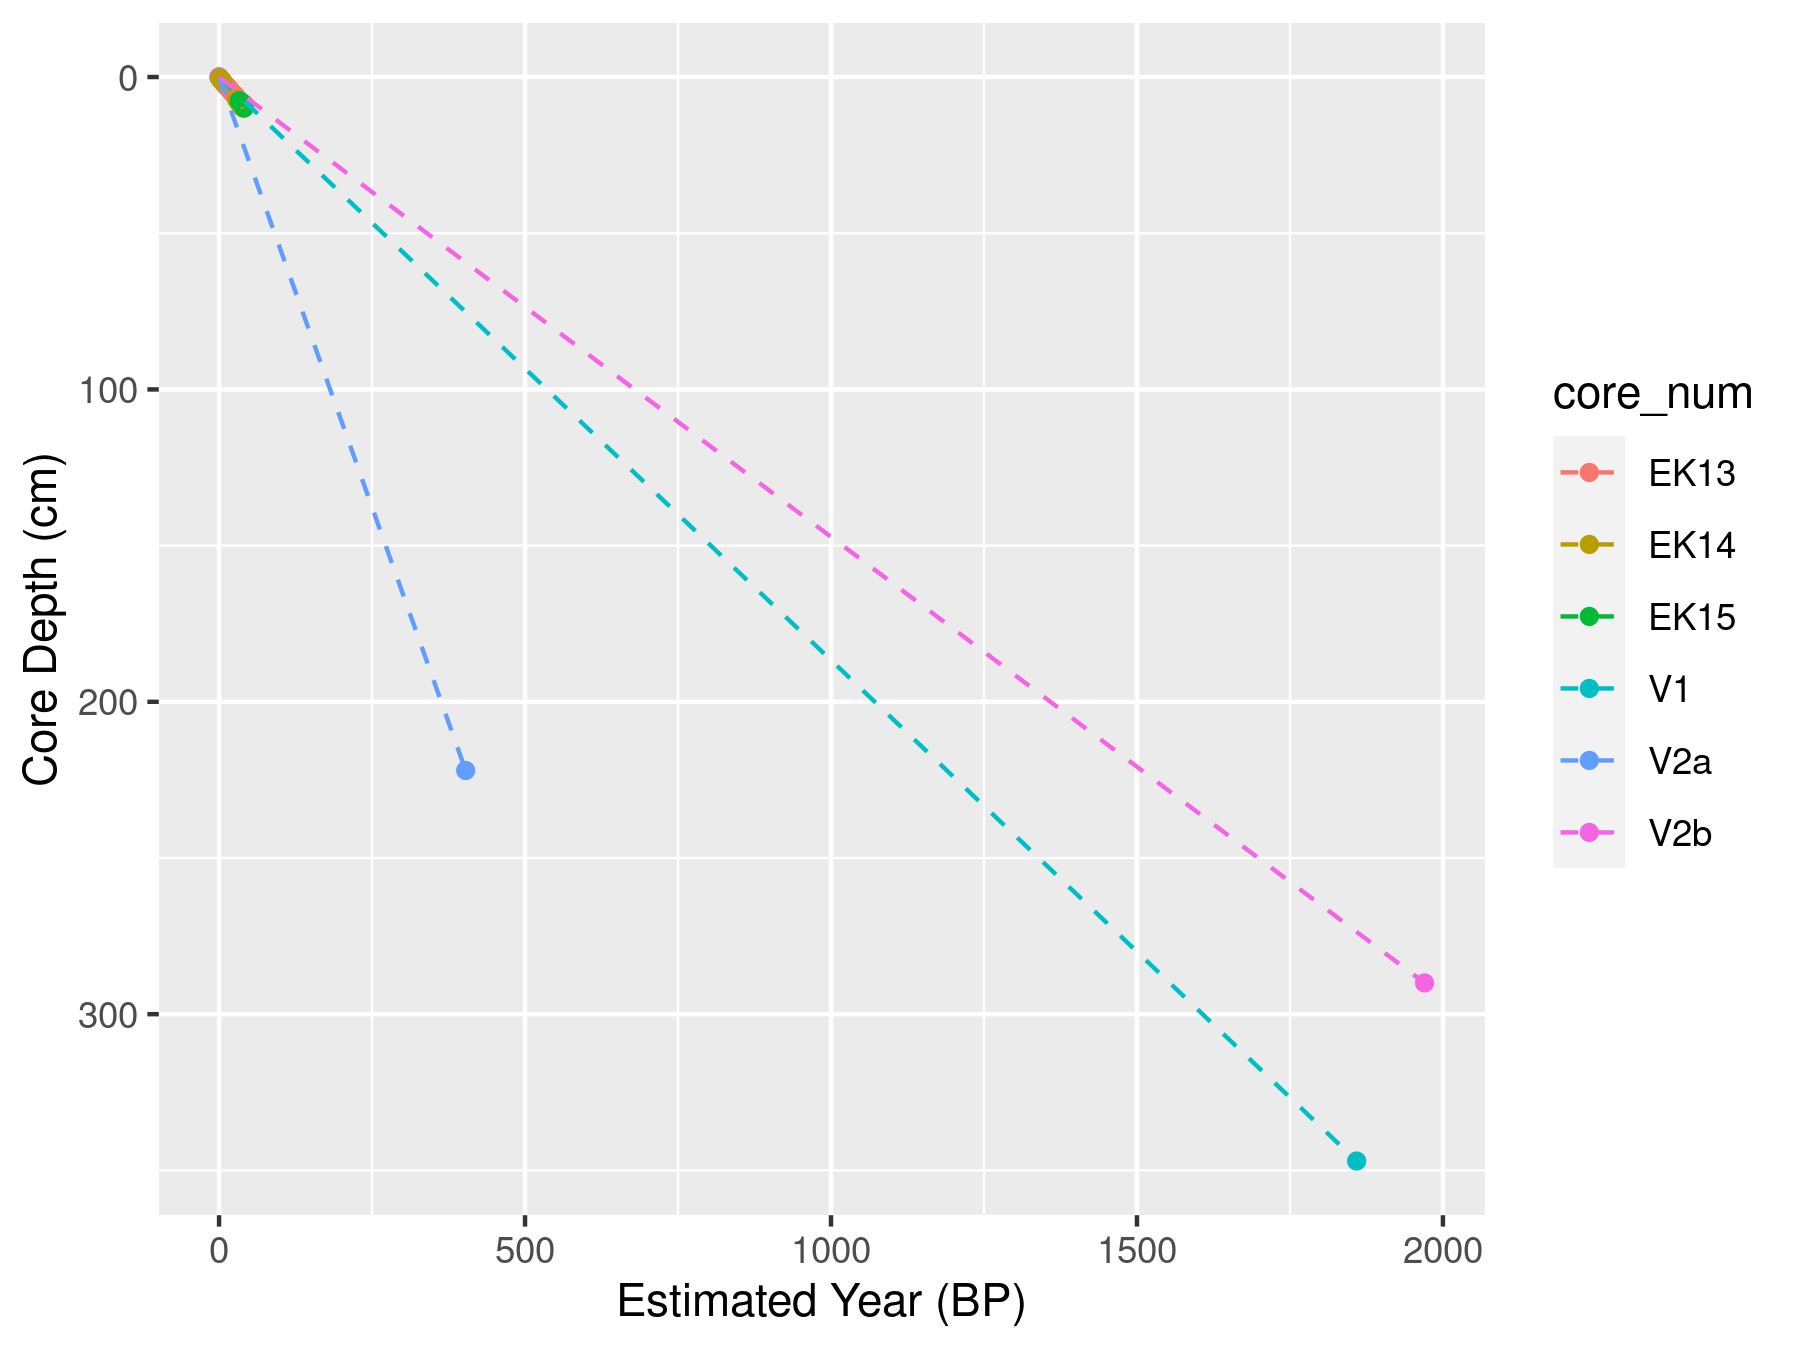
\includegraphics[width=1\linewidth]{figs/longcore_cumulative_depth_vs_estimated_year_w_ams_and_varve} 

}

\caption{Cumulative sediment accumulation rates for cores V1 and V2 using the median calibrated $^{14}$C AMS dates and lamanae couplet counting and thicknesses measurements. The error bars on the $^{14}$C dates are the two-sigma uncertainty range and the grey shading around the varve points is the 10\% counting error. Gaps between the varve chronology (points) denote periods that had indiscernable varves. The accumulation rate for the Ekman surficial core which has a maximum observed depth of 9 cm has been extrapolated using linear interpolation.}\label{fig:amsRates}
\end{figure}

By comparison with nearby lakes, accumulation rates in areas proximal to
river inputs in nearby Quesnel Lake were measured to be about 0.72 mm
yr\textsuperscript{-1} (see Figure 9 in \citet{Gilbert2012}). Sediment
inputs are expected to be lower in Quesnel Lake compared to Cariboo
Lake, with more arid and less glaciated portions of the Quesnel Lake
watershed contributing to that lower rate. The AMS accumulation rates of
1.76 ± 0.05 mm yr\textsuperscript{-1} and 1.37 ± 0.05 mm
yr\textsuperscript{-1} in Cariboo Lake are as expected for a smaller
watershed with a higher fraction of glacier cover compared to Quesnel
Lake. The AMS radiocarbon dates from samples V1 and V2 provide an
important control when interpreting the inferred temporal pattern of
sediment inputs to Cariboo Lake.

Three distinct sediment facies were observed in both V1 and V2:
discernible couplets, indiscernible couplets (disturbed facies) and
graded turbidite events. The similarity in couplet structure and
thickness between cores V1 and V2 and hydrology of Cariboo Lake strongly
suggested these are varves. This interpretation is also supported by the
two AMS radiocarbon dated samples from cores V1 and V2 which
corresponded reasonably well with the couplet count chronology at the
same depth (Figure \ref{fig:amsRates}). \textbf{A small difference
between the two chronologies was expected due uncertainties with
counting errors. The uncertainty of the laminae counting method is
inferred from Ekman surface cores by counting laminae down to a common
specifed depth of 5 cm for three Ekman cores (E12, E13, E14 - see Figure
\ref{fig:map-lake} for locations proximal to V1 and V2). The Ekman
laminae counting analysis resulted in an uncertainty estimate of the
counting method of about 10\% or 1 miscounted varve per 10 years. This
counting error of 10\% is higher than the varve counting error of 0.7\%
in \citet{Menounos2008c} and 0.7-6\% in \citet{Zolitschka1991}. In
\citet{Menounos2008c} and \citet{Zolitschka1991} varves were identified
using thin sections and may have contributed to a more accurate
chronology. The varve contacts observed in Cariboo Lake were strong and
there is reasonable confidence in counting. Missing varves may have
occurred if the spring nival high flows did not deliver a coarse-grained
laminae and false varves may occur if multiple high flows are observed
in a given year. However, the consistent nival flows of this basin shown
in Figure \ref{fig:cl-hydro} suggest multiple high flow events are rare.
This hypothesis is also supported by Figure \ref{fig:amsRates} which
shows a negative bias of the varve chronology compared to the calibrated
\textsuperscript{14}C age-depth model and suggests that missing varves
may be a larger source of error than false varves.}

Instantaneously deposited (event-based) turbidites were identified if
laminae/beds had D\textsubscript{50} grain size greater than 3 standard
deviations from the mean and/or thickness greater than 6 standard
deviations for V1 and 2 standard deviations for V2 from the mean. Figure
\ref{fig:varve-turb} examples show the difference in regular laminae
compared to an event-based turbidite bed. Turbidite beds observed in V1
and V2 were well defined and graded (see Figure \ref{fig:varve-turb},
d). These turbidite beds are similar in structure to those described in
\citet{sabatier2022} as originating from a flood, glacial lake outburst
flood, or delta collapse event. Since the Cariboo River upstream of
Cariboo Lake is filtered by headwater proglacial lakes, it is more
likely the turbidite beds at the distal V1 and V2 site are from
localized sidewall tributary floods. Collapse of the foreslope of an
oversteppened Cariboo delta is also possible.

\begin{figure}

{\centering 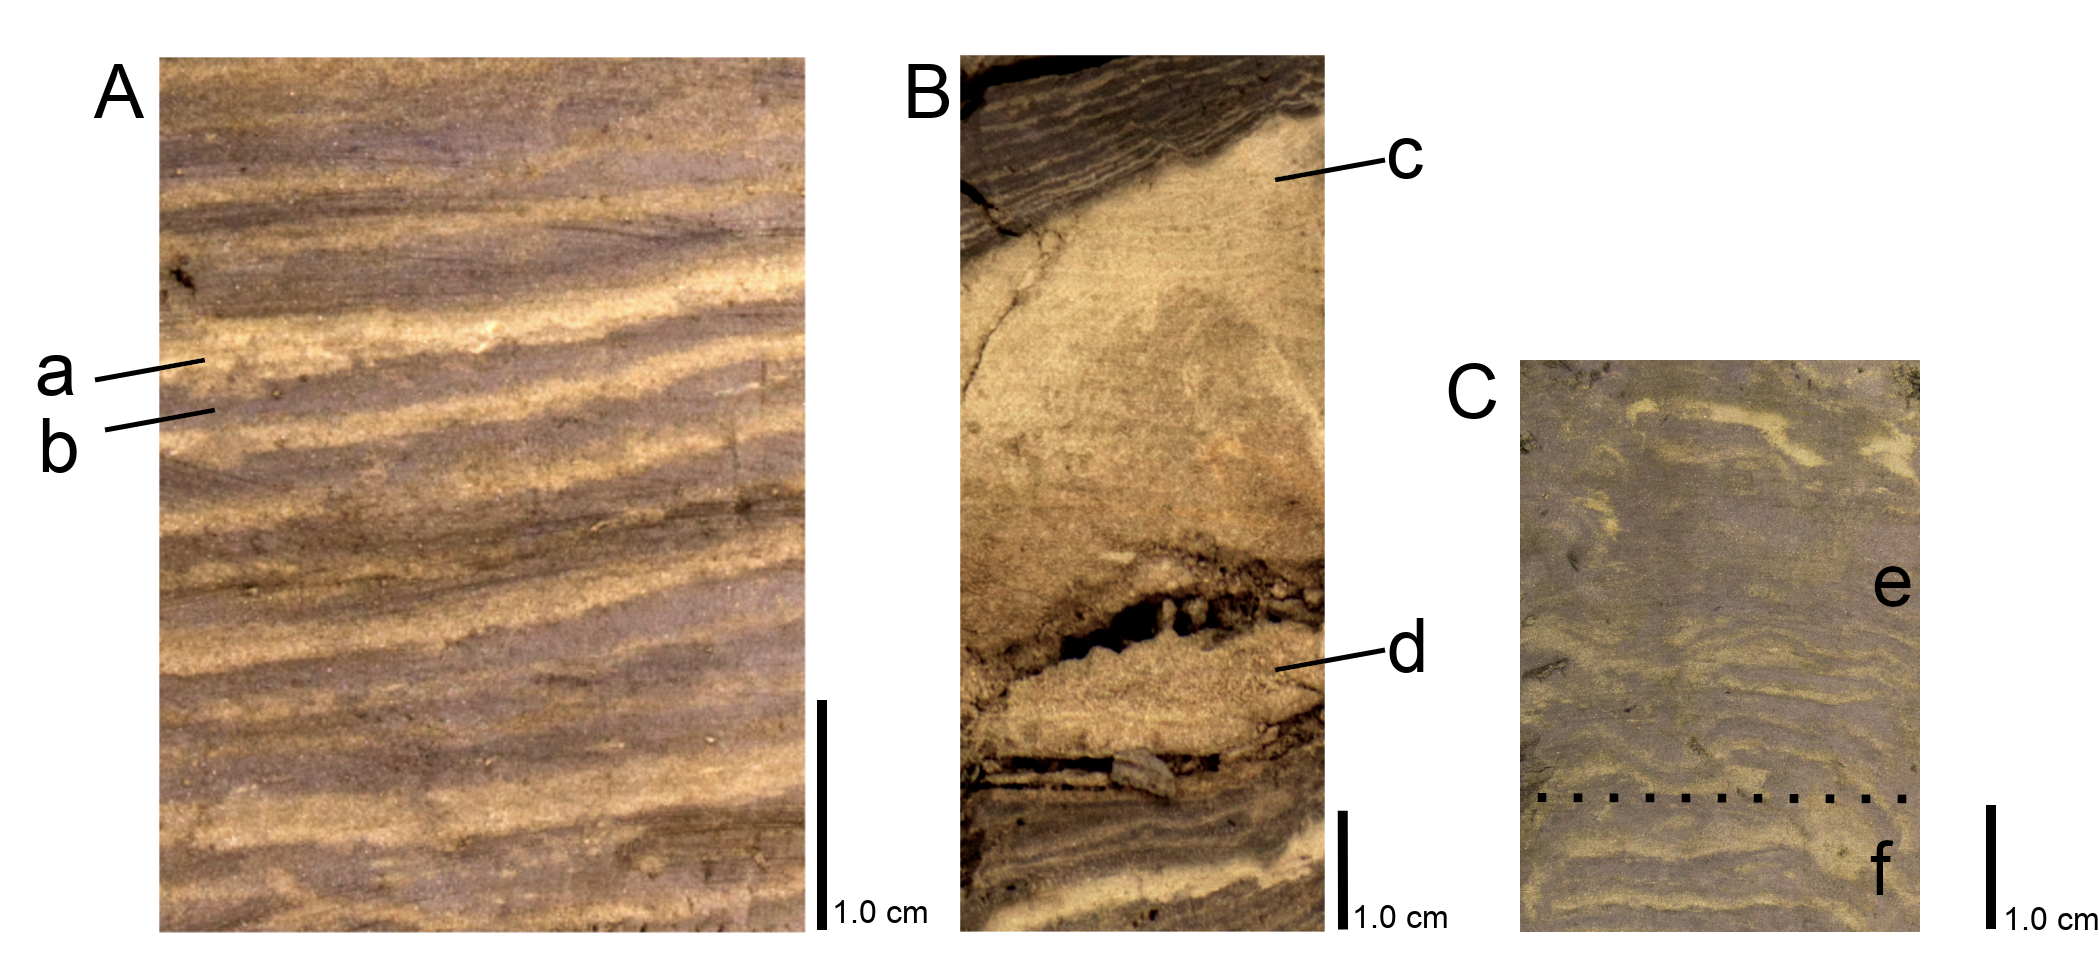
\includegraphics[width=1\linewidth]{figs/good_vs_flood_vs_disturbed_varves_} 

}

\caption{A. Example of regular laminae from V1 at a depth of 360 cm. B. a graded event-based turbidite bed from V2 at a depth of 230 cm. Features labeled within this figure include: ‘a’ high flow spring/summer freshet laminae, ‘b’ low flow winter laminae, ‘c’  top of the turbidite bed, and ‘d’ the bottom of the turbidite bed. C. shows massive beds ‘e’ over more distict laminations ‘f’.\label{tab:varve-turb}}\label{fig:varve-turb}
\end{figure}

Where possible the thickness, grain size statistics, and percent organic
matter (OM) were analyzed for each event layer. The turbidite bed grain
size, OM, and thickness shown in Table \ref{tab:turbTbl} illustrates the
high sediment flux during these events compared to the regular, annually
occurring couplets. The composition of sediment grains within the
event-based layers were all characterized by a coarser single mode with
less than 0.01\% clay, over 98\% silt and less than 1\% sand. The grain
size distribution for the regular couplet sediments is characterized by
a bi-modal distribution with an average composition of 16\% clay, 83\%
silt, and less than 1\% sand. Figure \ref{fig:turbScatter} shows that
some event layers are coincident in time between V1 and V2. Since each
of the event-based layers contain sediment deposited over a single,
potentially localized event, they were removed from subsequent trend
analyses of varve thickness, grain size, and percent organics.

\begin{longtable}[]{@{}
  >{\raggedright\arraybackslash}p{(\columnwidth - 10\tabcolsep) * \real{0.0676}}
  >{\raggedright\arraybackslash}p{(\columnwidth - 10\tabcolsep) * \real{0.2703}}
  >{\raggedleft\arraybackslash}p{(\columnwidth - 10\tabcolsep) * \real{0.2838}}
  >{\raggedleft\arraybackslash}p{(\columnwidth - 10\tabcolsep) * \real{0.1486}}
  >{\raggedleft\arraybackslash}p{(\columnwidth - 10\tabcolsep) * \real{0.1216}}
  >{\raggedleft\arraybackslash}p{(\columnwidth - 10\tabcolsep) * \real{0.1081}}@{}}
\caption{Sediment characteristics of regular laminae `Couplet (varve)'
compared to couplets classified as turbidite beds `Events' for V1 and
V2. The `Couplet (varve)' is the mean sediment characteristic for all
regular laminae couplets. The `Event mean' is the mean sediment
characteristic value for couplets classified as events, `Event sd' is
the standard deviation, and `Event n' is the number of turbidite
beds.\label{tab:turbTbl}}\tabularnewline
\toprule()
\begin{minipage}[b]{\linewidth}\raggedright
core
\end{minipage} & \begin{minipage}[b]{\linewidth}\raggedright
metric
\end{minipage} & \begin{minipage}[b]{\linewidth}\raggedleft
Couplet (varve) mean
\end{minipage} & \begin{minipage}[b]{\linewidth}\raggedleft
Event mean
\end{minipage} & \begin{minipage}[b]{\linewidth}\raggedleft
Event sd
\end{minipage} & \begin{minipage}[b]{\linewidth}\raggedleft
Event n
\end{minipage} \\
\midrule()
\endfirsthead
\toprule()
\begin{minipage}[b]{\linewidth}\raggedright
core
\end{minipage} & \begin{minipage}[b]{\linewidth}\raggedright
metric
\end{minipage} & \begin{minipage}[b]{\linewidth}\raggedleft
Couplet (varve) mean
\end{minipage} & \begin{minipage}[b]{\linewidth}\raggedleft
Event mean
\end{minipage} & \begin{minipage}[b]{\linewidth}\raggedleft
Event sd
\end{minipage} & \begin{minipage}[b]{\linewidth}\raggedleft
Event n
\end{minipage} \\
\midrule()
\endhead
V1 & D\textsubscript{50} (µm) & 7.64 & 9.68 & 0.80 & 5 \\
V2 & D\textsubscript{50} (µm) & 6.35 & 16.20 & 9.40 & 6 \\
V1 & OM (\%) & 4.75 & 4.67 & 0.53 & 3 \\
V2 & OM (\%) & 4.71 & 2.86 & 0.94 & 4 \\
V1 & Avg. Thickness (mm) & 2.39 & 10.32 & 4.24 & 5 \\
V2 & Avg. Thickness (mm) & 1.51 & 9.58 & 14.12 & 9 \\
\bottomrule()
\end{longtable}

The varve-based chronology is based on the counting of discernible
couplets with graded turbidite facies removed. Indiscernible couplets in
the disturbed-massive units makes interpreting the time elapsed over
each of these units difficult (see Figure \ref{fig:varve-turb} C). To
compensate for the depth intervals associated with the disturbed
sections, a 30-year moving average of sediment accumulation rates from
immediately above and below the disturbed sections were used to
interpolate accumulation rates over each facies (see method described in
Menounos et al., 2008). For core V1, laminae couplets were counted down
to a core depth of 343 cm, where the AMS radiocarbon organic material
was retrieved. \textbf{This resulted in a V1 couplet-derived age
estimated of 1419 ± 142 varve BP compared to the two-sigma calibrated
\textsuperscript{14}C age range of 1820-1918 cal BP. For core V2 a date
of 1792 ± 180 varve BP was estimated by couplet counting down to a core
depth of 281 cm which matches more closely with two-sigma calibrated
\textsuperscript{14}C age range of 1895-2043 cal BP. The better
alignment between the couplet counting age and the AMS derived age in V2
can be attributed to the higher degree of core disturbance in V1
compared to V2. Disturbed sections that had indiscernible couplets may
have resulted in the undercounting within core V1. Still, based on the
relatively close agreement between the AMS radiocarbon dated organic
material and couplet counting, laminae couplets in V1 and V2 are
considered to be deposited annually. Alignment closer than the observed
offset at V1 was not expected due to the uncertainty in the
\textsuperscript{14}C and varve based chronology. The varve estimate at
V2 is nearly within the uncertainty range of the calibrated
\textsuperscript{14}C age and therefore shows good agreement between the
varve and \textsuperscript{14}C chronologies.}

\begin{figure}

{\centering 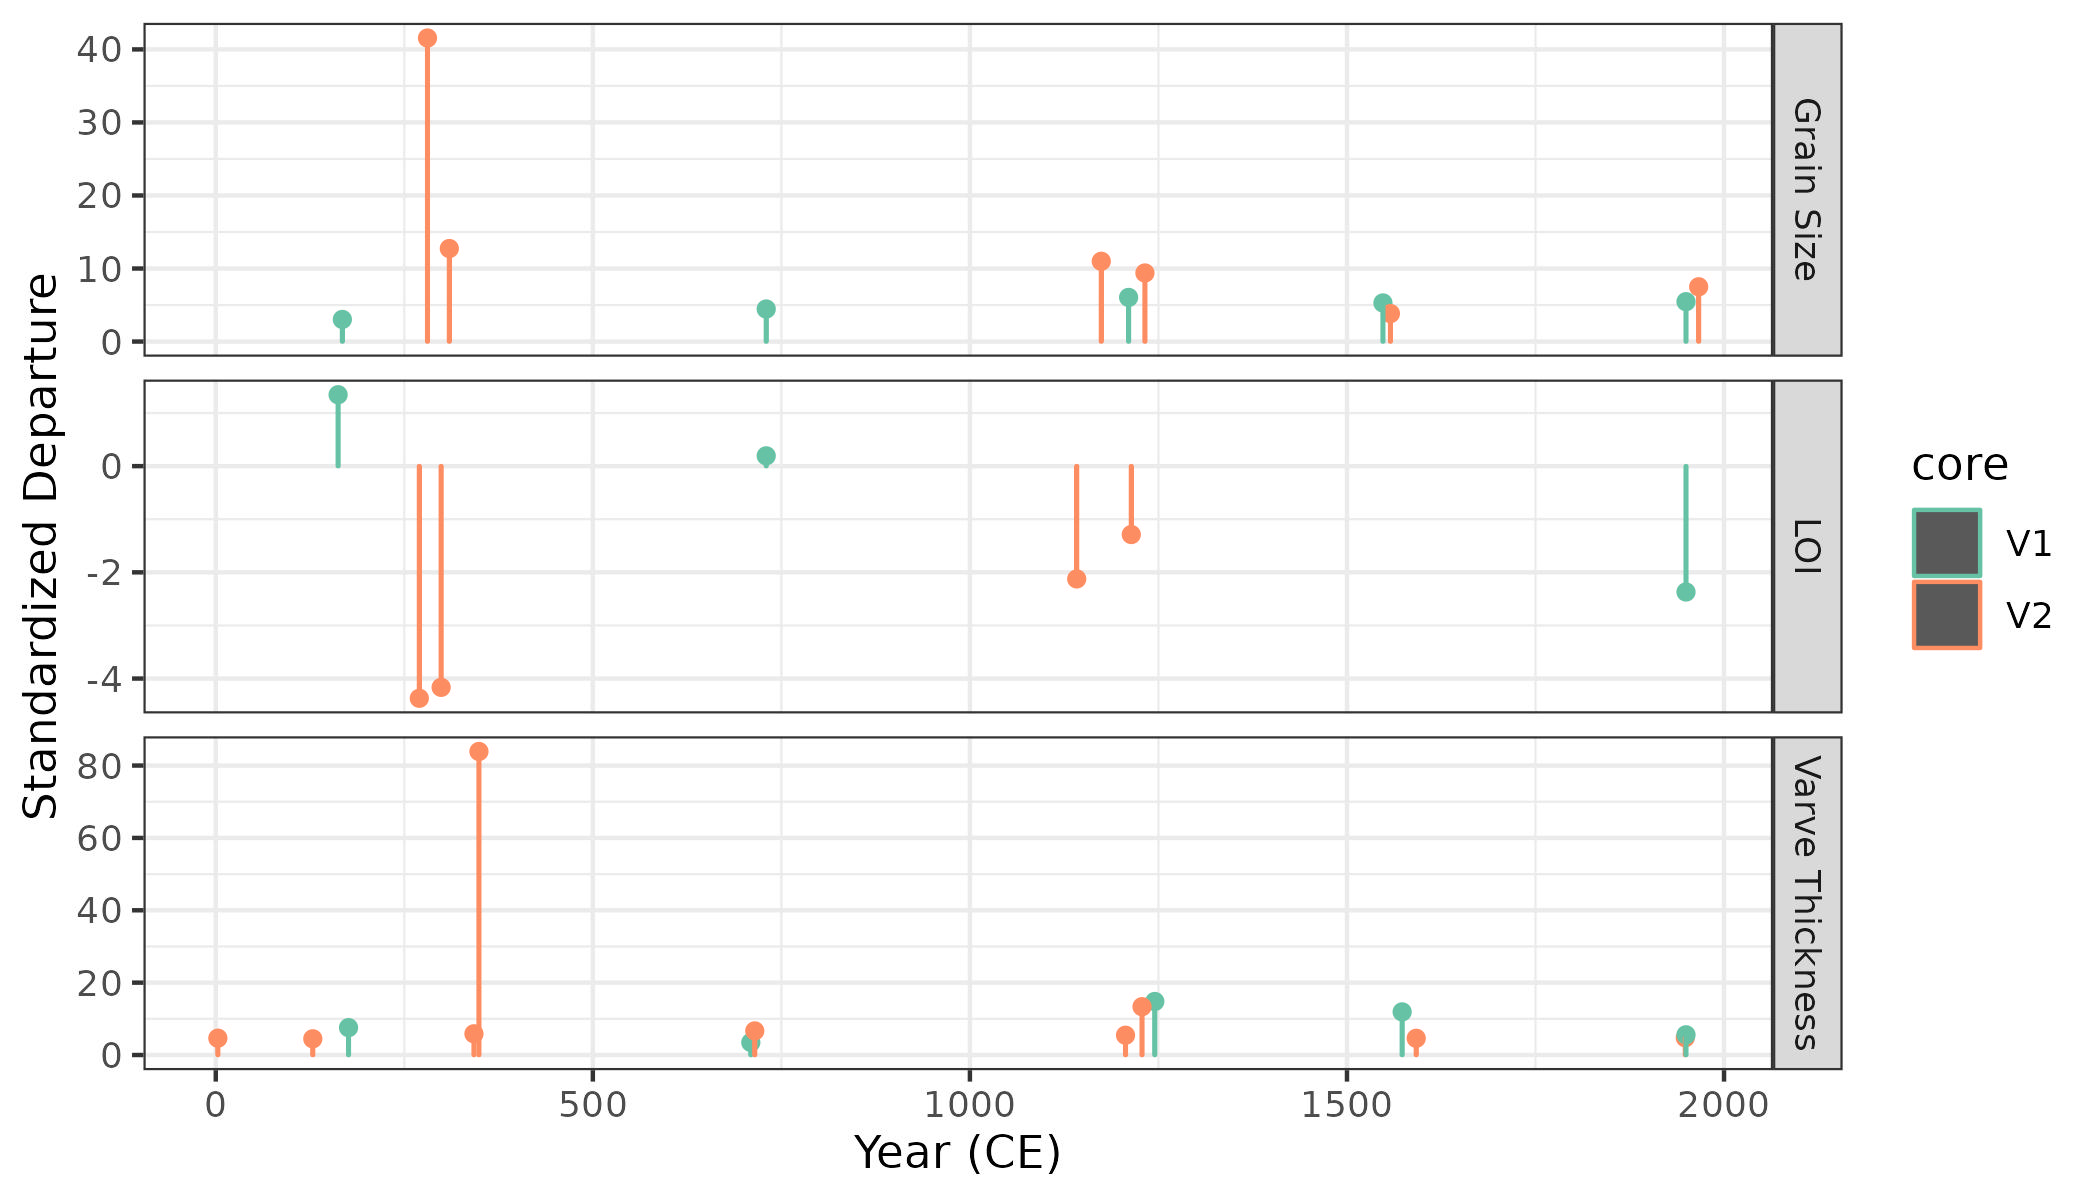
\includegraphics[width=1\linewidth]{figs/turbidite_plot} 

}

\caption{Timing and Standardized Departures of turbidite thickness, grain size, and OM for V1 and V2. Year (CE) is the estimated year using linear interpolation from the AMS radiocarbon dates.\label{turbScatter}}\label{fig:turbScatter}
\end{figure}

The basal age for each core is estimated using both the varve and using
a linear interpolation to extrapolate the \textsuperscript{14}C
chronology. The basal age of V1 at 378 cm is approximately 1537 ± 154
varve yr BP based on the varve chronology and the two-sigma calibrated
\textsuperscript{14}C range is 2016-2124 cal BP. The basal age of V2 at
282 cm is about 1797 ± 180 varve yr BP based on the varve chronology and
the two-sigma calibrated \textsuperscript{14}C range is 1902-2051 cal
BP. The closer alignment of the \textsuperscript{14}C and varve
chronology at V2 gives greater confidence in the timing of Holocene
sedimentation patterns for this core. While V1 has a greater spread
between the two chronology methods, we believe both cores are valid
estimates of late Holocene sediment accumulation patterns in Cariboo
Lake.

\hypertarget{sediment-laminae-statistics}{%
\subsubsection{Sediment Laminae
Statistics}\label{sediment-laminae-statistics}}

\textbf{A time series of varve thickness (as standardized departures) is
presented in Figure \ref{fig:varves-a}, using only discernible couplets.
Event-based turbidites have been removed and indiscernible facies are
represented as gaps. The chronology for this time series was derived
using a linear interpolation from the median calibrated
\textsuperscript{14}C date of each core (Table \ref{tab:amsDates}). The
mean varve thickness for V1 is 2.4 mm and for V2 is 1.5 mm. Thicker
varves are expected at V1 due to its closer proximity to the Cariboo
River delta. This is also supported by the thicker varves observed in
core E11 (proximal to V1) compared to E13 (proximal to V2) of 2.8 mm to
2.0 mm respectively. The time series of varve thickness measured from V1
and V2 and illustrates trends in suspended sediment delivery to Cariboo
Lake (Figure \ref{fig:varves-a}). The measured couplet thicknesses in
the two cores are plotted as standardized departures to facilitate
comparison between the two cores. In each plot a 30-year moving average
with a 1-year time step is plotted in black to emphasize decadal to
centennial patterns in accumulation rate departures. The 30-year average
varve thickness remains above average from 0 to 750 CE, for both V1 and
V2, with a stronger signal observed for V1 which is closer to the main
Cariboo River outlet. Below average varve thickness is observed at both
V1 and V2 from 750-1600 CE. After 1600 CE, trends in varve thickness
between the two cores depart, with V2 above average during the Little
Ice Age and V1 remains below average. Sub-centennial trends are not
reported due to the coarse temporal control for both V1 and V2.}

\begin{figure}

{\centering 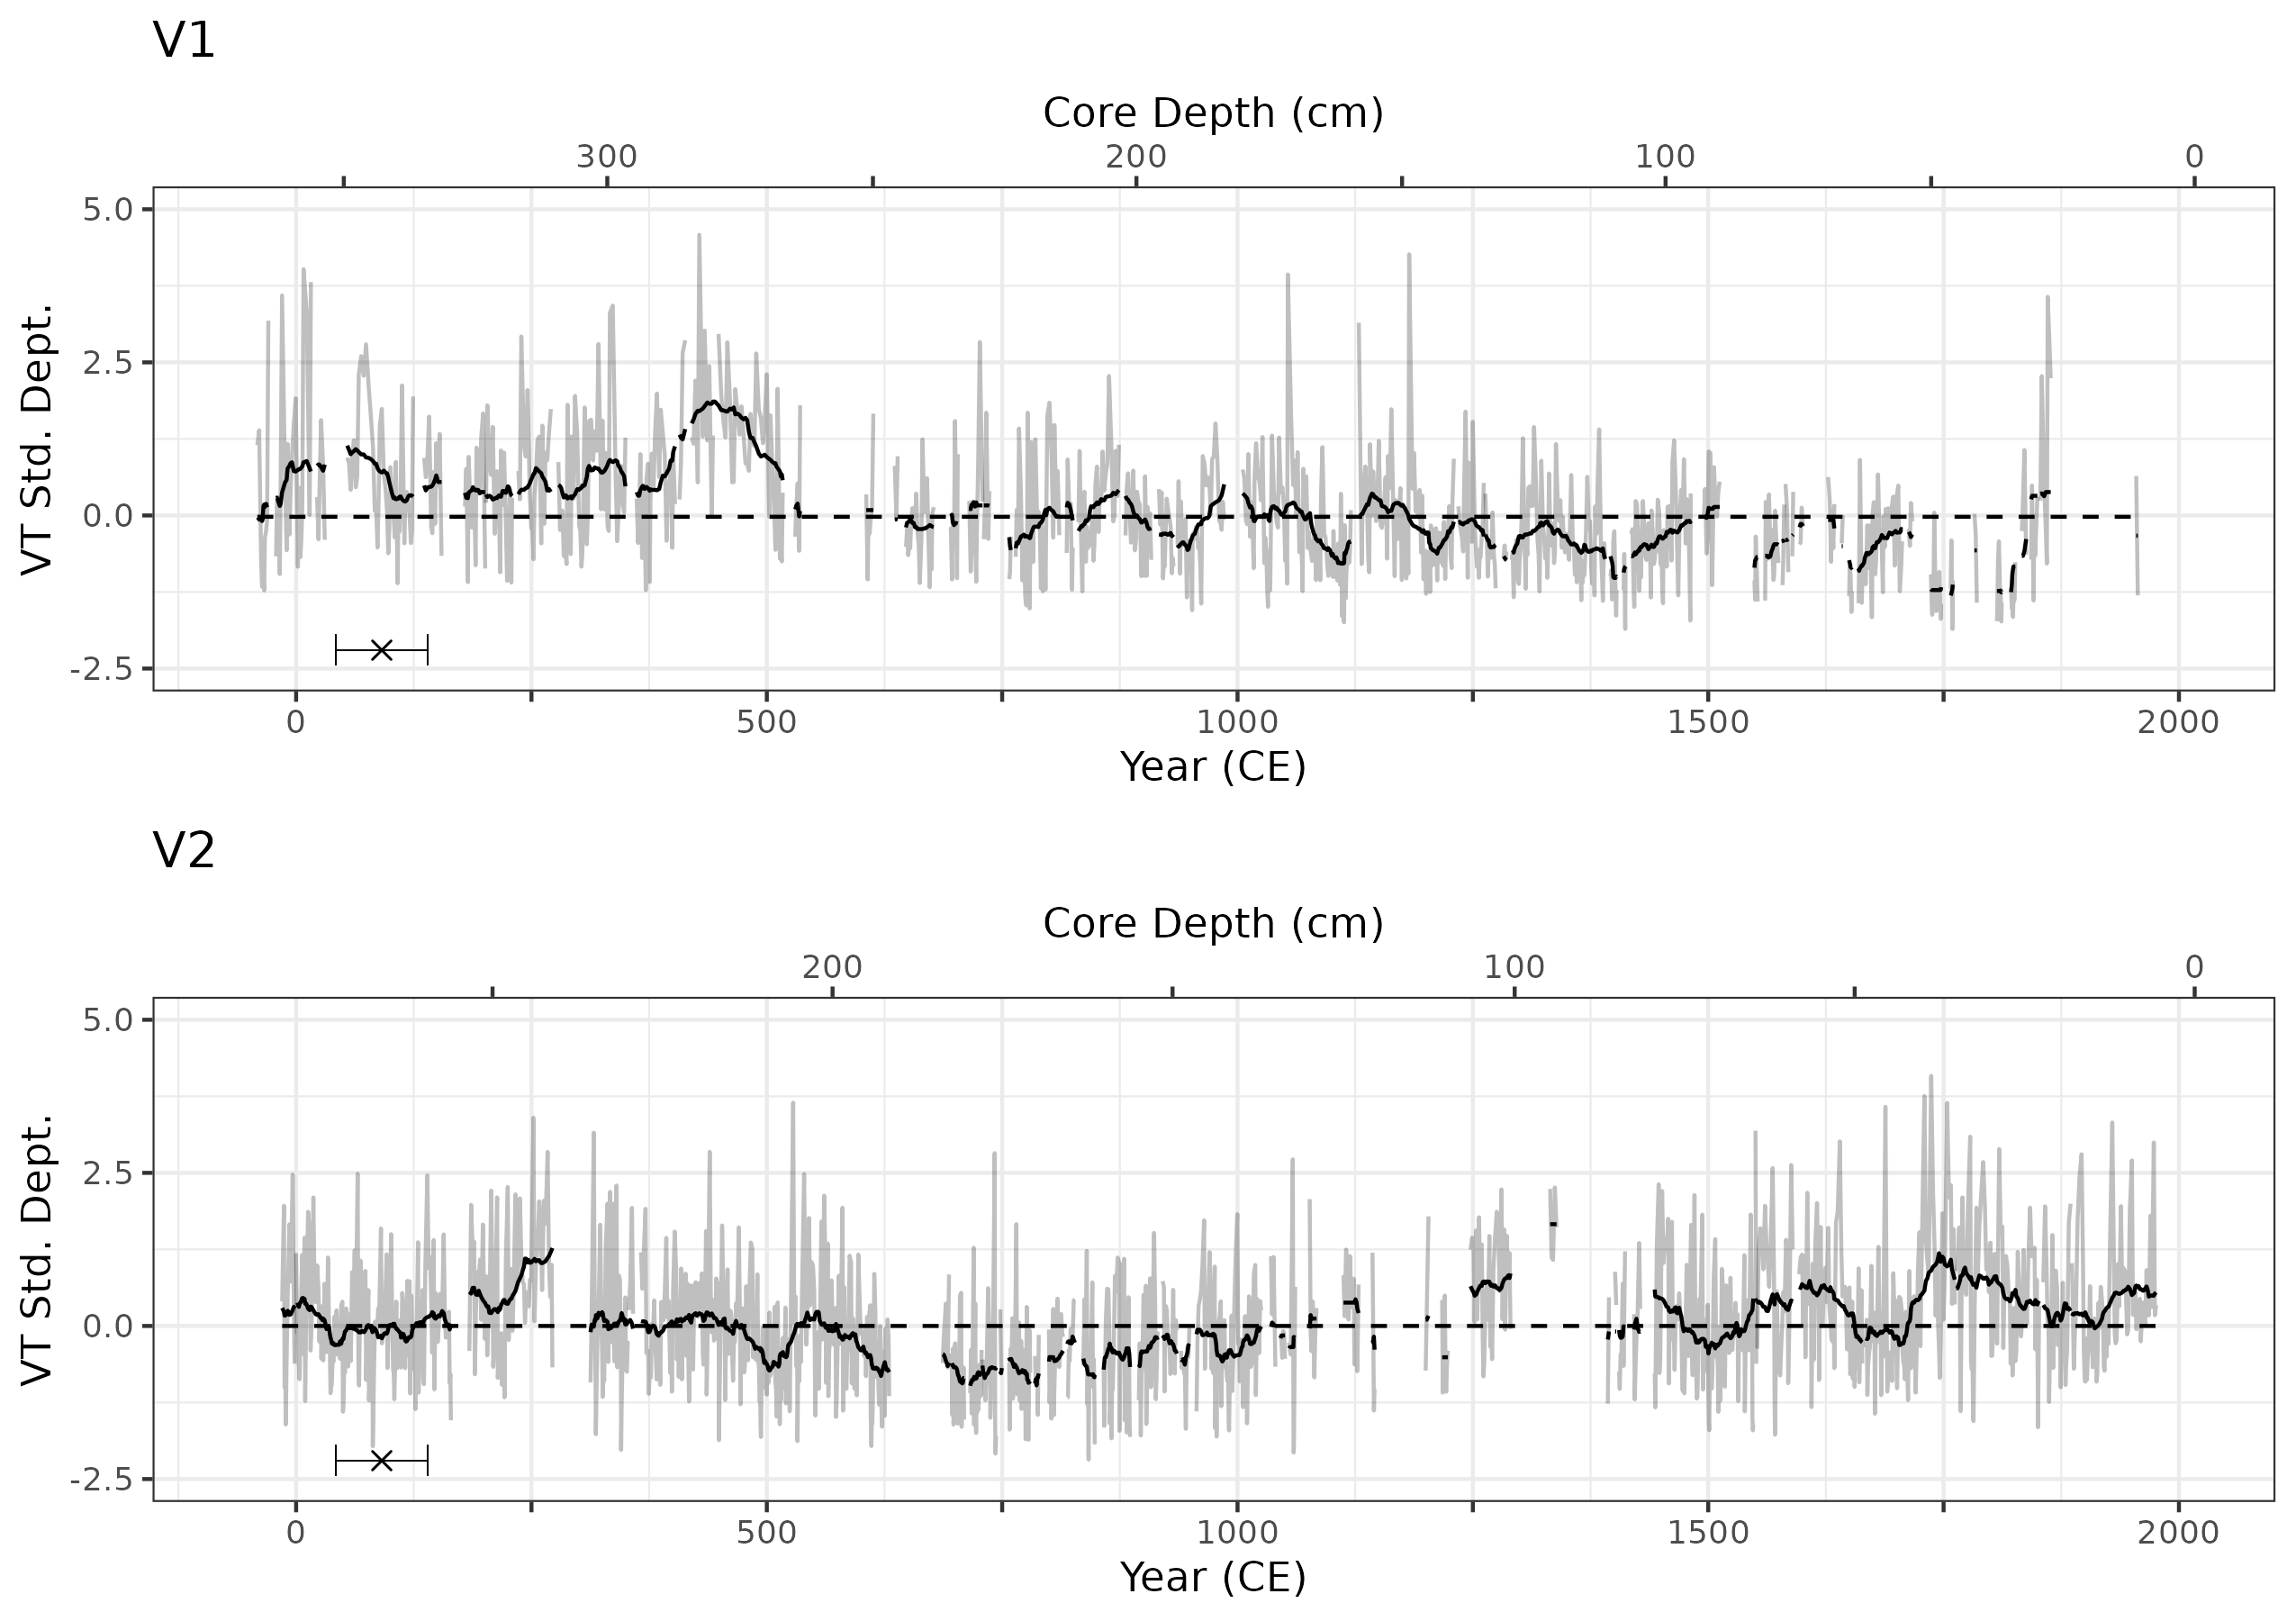
\includegraphics[width=1\linewidth]{figs/V1_V2_varvethickness_vs_depth_and_C14_est_yr_ma} 

}

\caption{Standardized departure from the mean varve thickness (VT) for cores V1 and V2. Events are removed from the record and disturbed facies are shown as blank gaps in the record. The gap width of disturbed facies was calculated using a linear interpolation from the AMS radiocarbon dates. The gray lines represent measured varve thickness at couplet (annual) resolution where available, the black line is a 30-year moving average. Gaps correspond to portions of the core that did not have discernible varves. The bottom axes, labeled Year (CE), was estimated using linear interpolation from the median calibrated $^{14}$C age. Laminae counting in V1 was not possible beyond the estimated date of ~1900 CE and beyond ~1970 CE in V2. The black X's on the bottom graph of V1 and V2 denote the AMS radiocarbon age (± dating error) and depth of the respective sample.\label{varves-a}}\label{fig:varves-a}
\end{figure}

\hypertarget{grain-size}{%
\paragraph{Grain Size}\label{grain-size}}

The mean D\textsubscript{50} grain size is 7.6 ± 0.01 µm at V1 compared
to 6.3 ± 0.01 µm at V2. The larger grain size and varve thickness at V1
compared to V2 is consistent with the spatial trends in sediment
delivery observed from the Ekman cores. While based on a limited number
of measurements compared to the varve thickness analysis, the temporal
pattern in standardized departures of D\textsubscript{50} grain size
between the two cores shows a consistent pattern (Figure
\ref{fig:particle}). Both V1 and V2 have above average grain size
between 0 to 700 CE and below average from 700 to 1500 CE. After 1500
CE, grain size follows an increasing trend with average to above average
grain size. V1 shows an earlier increase in grain size compared to V2.
While couplet thickness does not increase substantially over the LIA
interval, gain size does. Overall, grain size fluctuations at a temporal
resolution of about 100-years shows good correspondence between the two
cores over the last 2000 years.

\begin{figure}

{\centering 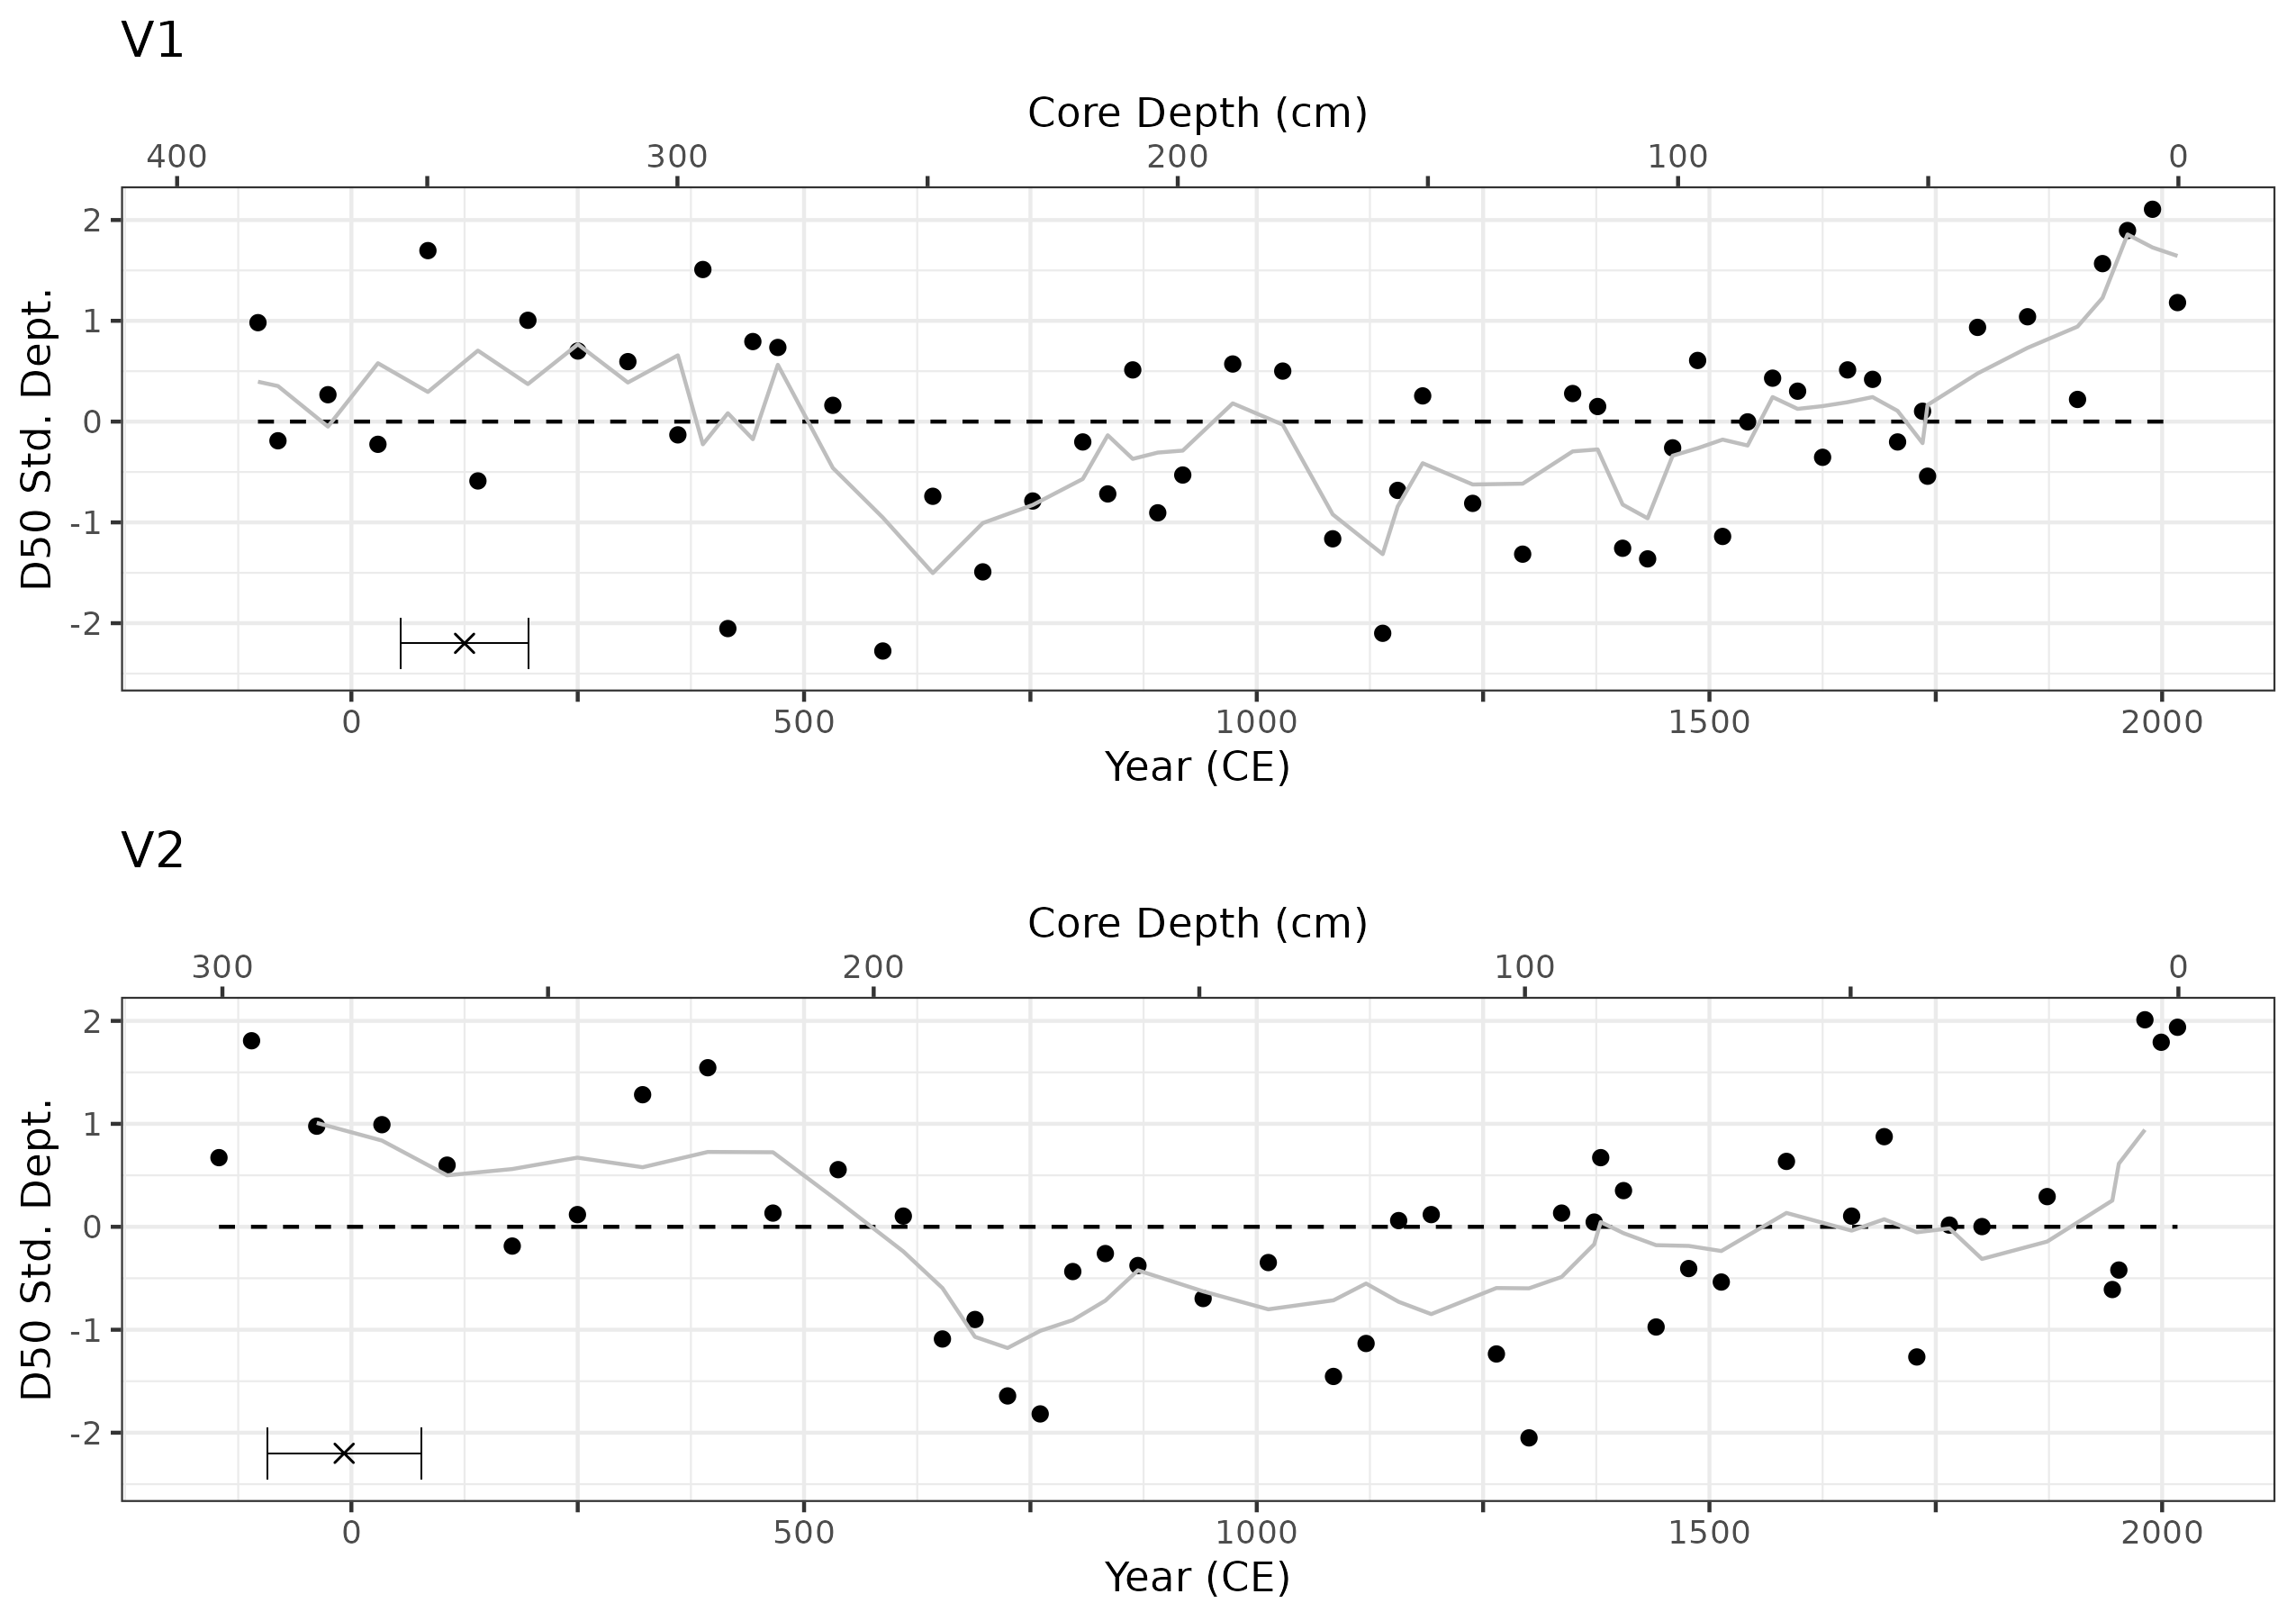
\includegraphics[width=1\linewidth]{figs/V1_V2_grainsize_vs_depth_and_C14_est_yr} 

}

\caption{Standardized departure from the mean D~50~ grain size for cores V1 and V2. The black points represent D~50~ grain size at 5 - 10 cm intervals and the gray line is the 3 sample (~125 year) moving average. The top axes, labeled Year (CE), was estimated using linear interpolation from the median calibrated $^{14}$C age. The black X's on the bottom graph of V1 and V2 denote the AMS radiocarbon age (± dating error) and depth of the respective sample.\label{particle}}\label{fig:particle}
\end{figure}

\hypertarget{organic-matter}{%
\paragraph{Organic Matter}\label{organic-matter}}

The average percent organic matter (OM) at V1 and V2 is similar at
4.76\% and 4.80\%, respectively, suggesting that the flux of
allochthonous organic material to the core locations is not dependent on
distance from the main Cariboo River as it is easily transported through
the lake due to low density. This is also supported by the Ekman OM
spatial analysis, where a systematic down-lake relationship was not
observed (Figure \ref{fig:ekmanSeds}, C). Figure \ref{fig:loi} shows the
percent OM for both V1 and V2. Higher levels of organic content are
shown in V1 and V2 from 0-1000 CE and mostly below average from
1000-2000 CE. Specific periods of above average OM for V1 occur around
CE 50-500, 650-1150, around 1300 and 1750-1850. OM in V2 matches above
average values in the interval CE 250-550 and 650-950. During the last
100 years both cores show a persistent decline in OM which could be
attributed to a relative increase in sediment delivery to Cariboo Lake
suggested by the increase in D\textsubscript{50} and varve thickness.
\textbf{As glaciers declined from peak LIA extents around 1750 CE
\citep{Leonard1997, Luckman2000g}, an increase in soil development,
vegetation growth and subsequent bank stability is expected which may
also contribute to a decline in OM as organic content is locked up as
needleleaf coniferous forest.}

\begin{figure}

{\centering 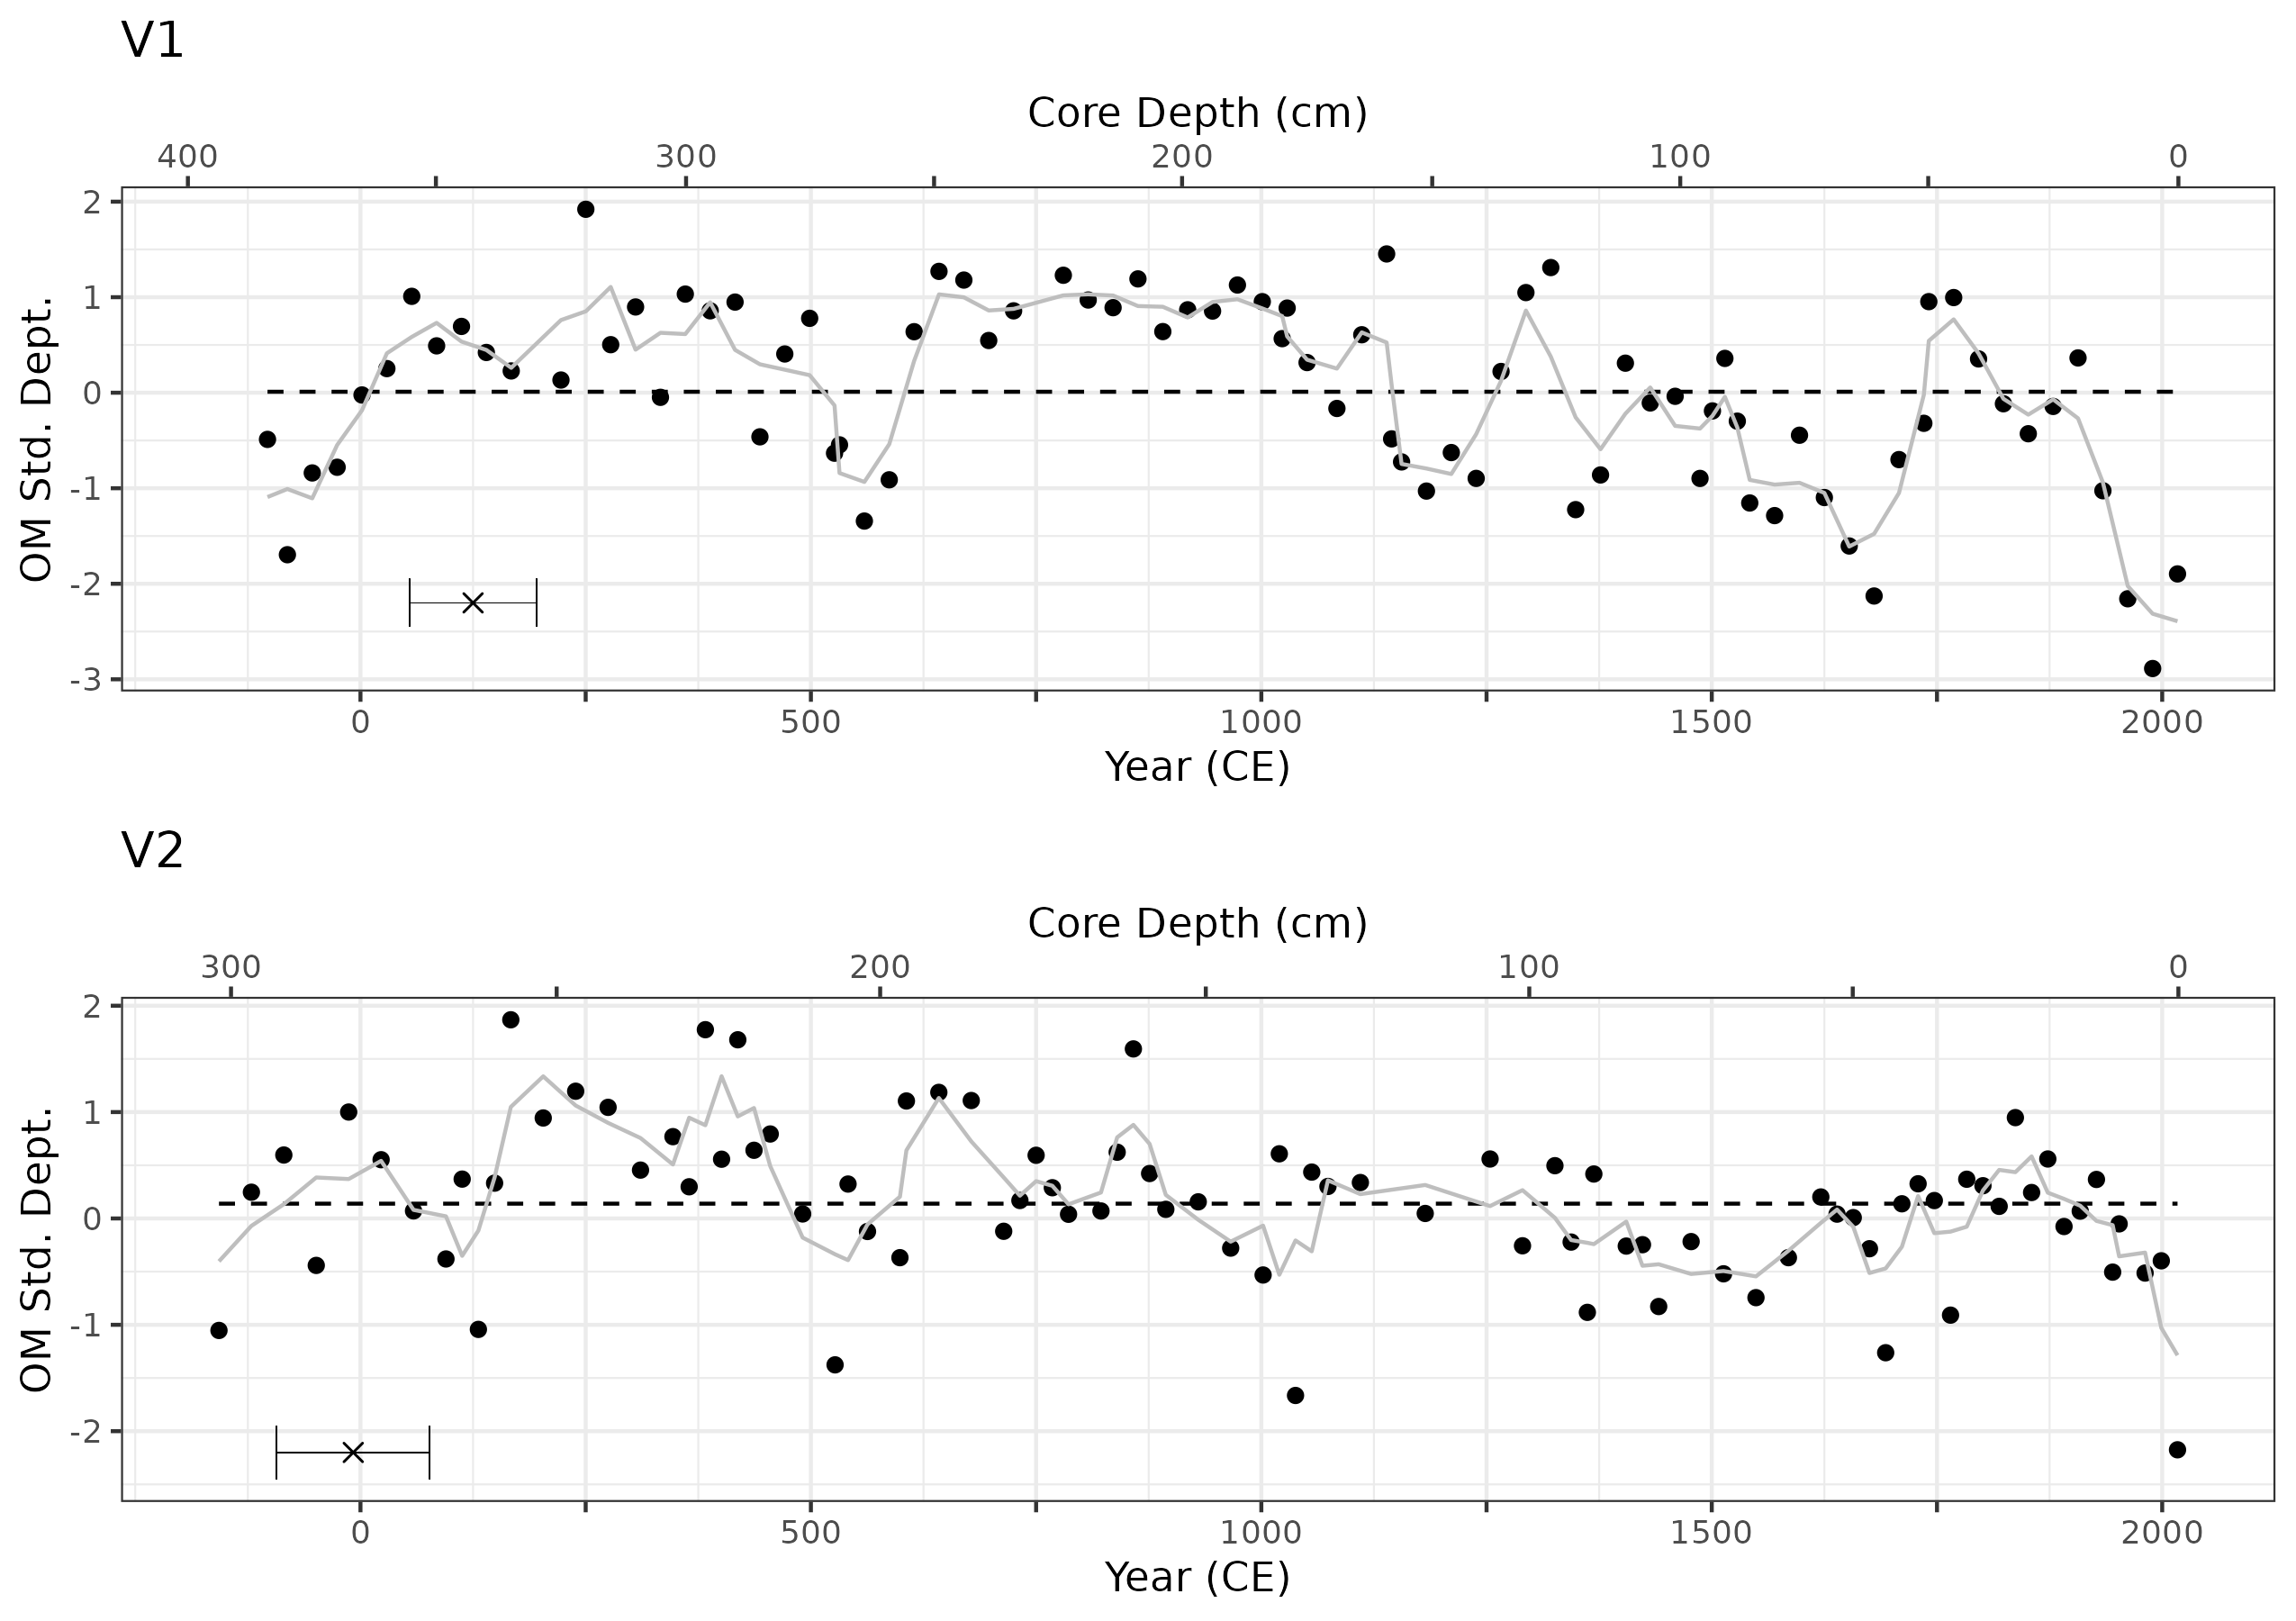
\includegraphics[width=1\linewidth]{figs/V1_V2_LOI_vs_depth_and_C14_est_yr} 

}

\caption{Standardized departure from the mean percent organic matter (OM) for cores V1 and V2. The black points represent percent OM at 2.5 - 5 cm intervals and the gray line is the 3 sample (~75 year) moving average. The top axes, labelelled Year (CE), was estimated using linear interpolation from the median calibrated $^{14}$C age. The black X's on the bottom graph of V1 and V2 denote the AMS radiocarbon age (± dating error) and depth of the respective sample.\label{loi}}\label{fig:loi}
\end{figure}

\hypertarget{discussion}{%
\section{Discussion}\label{discussion}}

Cariboo Lake was selected to test the utility of moderate sized
glacier-fed lakes as archives of accessible long-term and
high-resolution sedimentation input variability. Evidence of late
Pleistocene deglaciation in the Cariboo Lake region is provided by
coarse temporal resolution sub-bottom acoustic results. A maximum
deglacial sediment thickness of \textasciitilde35 m puts Cariboo Lake in
the middle to lower range of Holocene sediment inputs in Canadian
Cordilleran lakes \citep[see detailed discussion in][]{Gilbert2012}. The
study of smaller Mud Lake, in the Rocky Mountains to the east of Cariboo
Lake (Figure \ref{fig:map-basin} -- inset) was evaluated by
\citet{Hodder2006b}, who found the early phases of deglaciation and lake
sediment infill started just prior to 9.6 ka BP. \citet{Gilbert2012}
indicate deglaciation of the north and west arms of nearby Quesnel Lake
was likely complete by 8.6 ka BP. \citet{Menounos2009b} pointed to the
deglaciation of most of the Cordilleran ice sheet before 10.5 ka BP. The
Cariboo Lake acoustic results contribute to this regional record however
the inferred bottom dates present uncertainty in the actual timing.

Unlike many other deglacial sediment packages in Canadian Cordilleran
lakes, the sediment infill in Cariboo Lake has been subject to deep
trenching during deglaciation and the early Holocene (Figure 3c). The
troughs, with sediment infills occurring at different times, suggest the
presence of highly erosive but intermittent bottom currents during
deglaciation and into the very earliest Holocene. Energetic flow of cold
sediment-rich meltwater flow would be required suggesting proximity of
an actively retreating valley glacier. The absence of lower elevations
moraines in the valley upstream of Cariboo Lake might indicate rapidly
retreating ice into headwater locations. However, in general, moraines
indicative of stagnant ice fronts in lower elevation settings are not
common elsewhere throughout much of the eastern Cordillera suggesting
that valley glacier development was limited \citep{Menounos2009b}.

In contemporary ice-proximal lakes with extensive coverage of active
glaciers, high accumulation rates have been observed to be between 0.5 m
yr\textsuperscript{-1} \citep{Crookshanks2008} and as high as 1 m
yr\textsuperscript{-1} \citep{Gilbert1997}. Similar high accumulation
rates in the late-glacial are inferred to have occurred in Quesnel Lake
\citep{Gilbert2012}, resulting in a thick pre-Holocene sediment package.
This evidence for high pre/early Holocene accumulation rates in Quesnel
Lake from large dynamic glaciers suggests that high accumulation rates
are also likely for Cariboo Lake during this time and is supported by
the acoustic data presented here.

Sub-bottom acoustic records from Transect B shown in Figure
\ref{fig:acoustics}, which is proximal to the V1 core, indicate an
upward transition from massive-unlayered (Facies A) to well-layered
sediments (Facies B) at a depth of about 20 m. Assuming a maximum
Holocene sediment accumulation rate of approximate 1.9 mm
yr\textsuperscript{-1} from V1, this would put this transition at about
10.5 ka BP. The massive structure of Facies A is inferred to be due to
high rates of sediment delivery as glaciers retreated upvalley during
the early Holocene after the formation of the deep trenches. The
well-layered sediment of Facies B, along with the continuation of
laminae couplets observed in cores V1 and V2 over the last 2 ka,
suggests that glaciers reduced in extent at the start of the Holocene
but did not disappear completely. It is possible during this transition
from Facies A to B, glaciers retreated above Lanezi Lake resulting in a
more sediment filtering and thus a reduction in sediment delivery and
the beginning of seasonally derived laminae couplet formation within
Cariboo Lake.

Transect C, shown in Figure \ref{fig:acoustics} is located in-between
cores V1 and V2, has \textasciitilde15 m of well layered sediment
overlying a massive unlayered lower Facies A. Using a combined V1 and V2
average Holocene sediment accumulation rate of 1.7 mm
yr\textsuperscript{-1} in this region of the lake, puts the transition
from Facies A to B at around 9 ka BP, slightly later than the Transect B
estimate. However, sediment accumulation rates is generally lower across
western Canada prior to the Neoglacial, due to widespread glacial
activity and warm temperature during the early Holocene
\citep{Steinman2019, Menounos2004, Koch2007a, Osborn2007, Luckman1988, Luckman1993}.
Therefore, the estimated basal ages of Facies A and B, estimated from
sedimentation rates over the last 2 ka from the long cores presented
here, may be much older if the actual sedimentation rates were used. The
timing of the transition between these two facies is similar to the
onset of deglaciation and start of the Holocene sediment package within
Mud Lake, BC \citep{Hodder2006b} around 9.6 ka BP, at Moose Lake, BC
\citep{Desloges1999} around 10.3 ka BP, at Quesnel Lake, BC
\citep{Gilbert2012} around 8.6 ka BP, and at the Upper Bow River, AB
\citep{Leonard1999} around 11.7 ka BP. Warming in the early Holocene,
around 9.10-6.70 ka BP in the Canadian Rockies, specifically,
\citep{Luckman1986} and British Columbia, generally,
\citep{Clague1989, Steinman2019} led to two possible sedimentation
regimes. Where glaciers persist in the Canadian Rockies through the warm
period resulting in more regular seasonality of sediment inputs and
laminae couplet formation \citep[e.g.~Mud Lake,][]{Hodder2006b} and
where glaciers disappear during the warm period, leading to much lower
accumulation and seasonality \citep[e.g.~Moose Lake,][]{Desloges1999}.

Records of sub-bottom acoustic records from Cariboo Lake present coarse
temporal scale resolution of continuous sedimentation rates throughout
the Holocene. Higher resolution AMS dated sediments from the much
thinner sediment package in the west arm of Quesnel Lake, located in the
Cariboo Mountains (Figure \ref{fig:map-basin}), also showed a very
consistent mean rate of sedimentation throughout the entire Holocene
\citep{Gilbert2012}. Contrasting somewhat from this pattern are results
from \citet{Menounos2004} and \citet{Desloges1999} who note that early
to mid-Holocene sediment accumulation rates in the southeastern Canadian
Cordillera were lower than the late-Holocene Neoglacial period. However,
those shifts come from watersheds with much higher percentages of
glacier ice cover (\textasciitilde15-40\%) coupled with the probable
disappearance of glaciers during the warmer hypsithermal. Therefore, any
extrapolation of timing to the early sediment record of Cariboo Lake
remains speculative.

Sediment inputs to Cariboo Lake are mainly delivered via the Cariboo
River delta and thus changes in the whole of the Cariboo Lake watershed
would be expected to be important. In contrast, inputs of sediment from
the small tributary watersheds that boarder Cariboo Lake are controlled
by more localized, watershed-specific responses. Although coarser
grained sediments from discrete turbidite flows are found proximal to
sidewall tributary deltas (Figure \ref{fig:ekmanSeds}), they are only
transferred to deep lake deposits during episodic events (Figure
\ref{fig:turbScatter}). \textbf{After removal of instantaneous
turbidites, the long core sediment records are thought to be most
representative of watershed wide trends in river discharge influenced by
temperature and precipitation rather than isolated events and inputs
from nearby tributaries and hillslopes.} The long core (V1 and V2)
sediment is composed of nearly 99\% silt and clay resulting in laminae
couplets that are inferred to have been delivered via suspended sediment
from the main Cariboo River. Therefore, trends observed in sediment
accumulation at cores V1 and V2 likely best represent waterside-wide
climate and glacier activity.

While cores V1 and V2 do not produce identical results, it is likely the
sediment yield data from these cores are within the range of 7-21\%
error reported in Evans and Church (2000) for other alpine lakes in
British Columbia. The inferred error of cores V1 and V2 is attributed to
the spatial heterogeneity of sediment accumulation across the Cariboo
Lake, and is likely on the lower end of this error range due to its
simple basin morphology. Retrieving more than two good long core
sedimentary sequences, could have provided a better estimate in the
error of sediment accumulation, however, the logistical demands of
retrieving more cores prevented this.

There is a documented range of late Holocene clastic sediment
accumulation rates in glacier-fed lakes from across the Canadian
Cordillera. Highest rates of \textgreater{} 2 cm/yr are observed in
ice-contact to ice-proximal lakes of various sizes
\citep{Desloges1994d, Crookshanks2008}, to relatively low rates of
\textless{} 1 mm yr\textsuperscript{-1} \citep{Gilbert2012}. The range
in accumulation rates has been understood to be a result in the
variability of sediment production from glacier processes, the steepness
of topography \citep{Ballantyne2002}, the persistence of ice cover and
the degree of basin connectivity enhancing or impeding delivery of
sediment down valley \citep{Wohl2019}.

In the Cariboo Lake basin, the combination of upper watershed area,
intervening storage, glacier cover and lake size are considered optimal
during this period for the relatively consistent formation of clastic
varves. The Cariboo River has two main tributaries, the Upper Cariboo
River and the Matthew River which are connected to high alpine peaks and
glaciers providing a significant source of sediment (see Figure 2).
Lanezi, Sandy and Ghost lakes act as sediment traps eliminating the
transfer of coarse sediment and limiting the transfer of finer sediment
from the glacier sediment production zones. This results in sediment
accumulation rates that are on the low-end for the southeastern
Cordillera \citep{Hodder2006b}. Although connectivity is limited, there
are sufficient seasonal contrasts in suspended sediment flux to produce
couplets (annual varves) in the main basin of Cariboo Lake over the last
two millennia. This is unlike the west arm of Quesnel Lake where
sediment rates are 2 to 3 times lower due to significant storage in the
much larger upper watershed.

Lake sediment chronologies typically vary in their sensitivity to
regional fluctuations in temperature and precipitation, from annual
resolution in lakes with higher accumulation rates
\citep[e.g.][]{Menounos2008c} to centennial-scale in lakes with low
accumulation rates \citep[e.g.][]{Desloges1999}. Figure
\ref{fig:proxy-comparison}a shows the (inferred) varve thickness
chronology reconstructed as standardized departures from cores V1 and
V2. There is a significant amount of noise in the record, typical of a
filtered sediment transport system \citep[e.g.][]{Jerolmack2010}, so a
lower resolution 30-year moving average is superimposed on the raw
couplet thickness data in Figure \ref{fig:proxy-comparison}a. Figure
\ref{fig:proxy-comparison}b and \ref{fig:proxy-comparison}c show the
lower-resolution temporal patterns in D\textsubscript{50} grain size and
organic matter content, respectively. These trends are compared against
the \citet{Moberg2005} regional climate proxy re-analysis for the
northern hemisphere (Figure \ref{fig:proxy-comparison}d),
\citet{Solomina2016} western Canada peak glacier extent estimates
(Figure \ref{fig:proxy-comparison}e), and \citet{Ljungqvist2016}
hydroclimate anomaly estimates for the northern hemisphere (Figure
\ref{fig:proxy-comparison}f). Most of these are at resolutions of
centennial scale or lower.

\textbf{For Cariboo Lake, above average varve thickness, grain size, and
organic matter are observed for both V1 and V2 from 2.0-1.3 ka BP. In
the southern Coast Mountains of British Columbia
\citep{Koch2007a, Osborn2007, Allen2007, Clague2010} and in the Interior
ranges and Rocky Mountains \citep{Luckman1993, Luckman1995} glaciers
were generally more extensive prior to 2.0 ka BP than present day. More
recently than 2.0 ka BP, there is evidence of the First Millennium
Advance (FMA) primarily from the Coast Mountains
\citep{Reyes2006, Osborn2007} with more recent evidence emerging from
the Interior Ranges \citep{Maurer2012b}. These results cover a range of
advance dates between 1.80 and 1.30 ka BP. The increase in sediment
production and sediment availability due to extensive glacier advance
and then retreat from the FMA may be reflected here by the increase in
varve thickness and grain size in the Cariboo Lake record (Figure
\ref{fig:proxy-comparison}). Observations of an increase in clastic
sedimentation rates in the Rocky Mountains were also observed around 1.8
ka BP in Hector Lake \citep{Leonard1997}. \citet{Maurer2012b} show that
the Castle Creek Glacier intermittently advanced into On-off Lake and
over the Cariboo River watershed divide throughout the late-Holocene
between 2.73-2.35, 1.87-1.72, and 1.53-1.42 ka BP (Figure
\ref{fig:proxy-comparison}). Additional contributions of sediment from
the Castle Creek Glacier would help contribute to above average varve
thickness and grain size observed in Cariboo Lake from 2.0-1.3 ka BP.
However, the above average organic matter observed in Figure
\ref{fig:proxy-comparison} is atypical during an increase of clastic
sediment delivery, but could be explained by some contributions from
increased soil erosion below treeline during a time of higher
precipitation rates and subsequent high spring freshet flows.}

\textbf{The coarsening trend of grain size from 750-1000 CE in Cariboo
Lake is consistent with evidence of an early Little Ice Age (LIA)
glacier advance centering around 1250 CE in the Canadian Rockies
\citep{Luckman1995, Osborn2001, Leonard1997}, in the Cariboo Lake basin
around 1040-1160 CE \citep{Maurer2012b}, and more broadly across western
Canada around 1100 CE \citep{Solomina2016} (Figure
\ref{fig:proxy-comparison}, D). This period of increased glacier
activity also corresponds with the highest temperature anomaly of the
Northern Hemisphere MCA \citep{Moberg2005} (Figure
\ref{fig:proxy-comparison}). However, \citet{Ljungqvist2016} estimate
precipitation to be above average around this time which could have
contributed to an increase in glacier extent if corresponding
temperatures were low enough. \citet{Steinman2012} studied two lakes in
northern Washington, USA which also support above average precipitation
for this region during the MCA. Although temperatures are reported as
slightly above average during the MCA \citep{Moberg2005} for the
Northern Hemisphere, the increase in glacier activity during this time
may have been a result of increased winter precipitation which may have
lowered the ELA of glaciers in the Cariboo Lake basin.}

\textbf{The second glacier advance of the LIA, which centers around 1850
CE in the Canadian Rockies \citep{Luckman2000g, Leonard1997} coincides
with thicker and coarser varves, and a reduction in organic matter in
Cariboo Lake (Figure \ref{fig:proxy-comparison}). The change in varve
thickness, grain size, and organic matter begins earlier for V1 at
around 1750 CE compared to V2 which begins to change around 1825 CE. The
discrepancy in the sediment characteristic trends between the two cores
is considered small given the uncertainty in couplet counting. Overall,
the response of varve thickness, grain size, and organic matter to the
second advance of the LIA around 1850 CE exhibits a stronger response
compared to earlier phases of the LIA.}

\textbf{Temperature anomalies for the Northern Hemisphere reported by
\citet{Moberg2005}, are also most negative from 1500-1750 CE. The dryer
conditions reported by \citet{Steinman2012} from 1600-1900 CE, 500 km
south of Cariboo Lake in Castor and Lime Lakes could be attributed to a
strong negative temperature anomaly. These records suggest there was a
strong influence of the LIA climate on glacier activity in the region
compared to the rest of the 2 ka record. Following the LIA, around 2000
CE a dramatic decline in organic matter and increase in grain size is
observed suggestive of high magnitude clastic sediment delivery. This
could be attributed to the increase of sediment availability as glaciers
retreated more rapidly from LIA extents and exposed stores of clastic
sediments \citep{Beedle2015}. However, hydraulic mining practices during
the Cariboo Gold Rush and deforestation began during the late 1800s and
they also may have contributed to this rapid increase. Human disturbance
related controls on sediment inputs for the last 100 years or more are
known to confound the climate-glacier-sediment output signal
\citep{Beedle2015}.}

\begin{figure}

{\centering 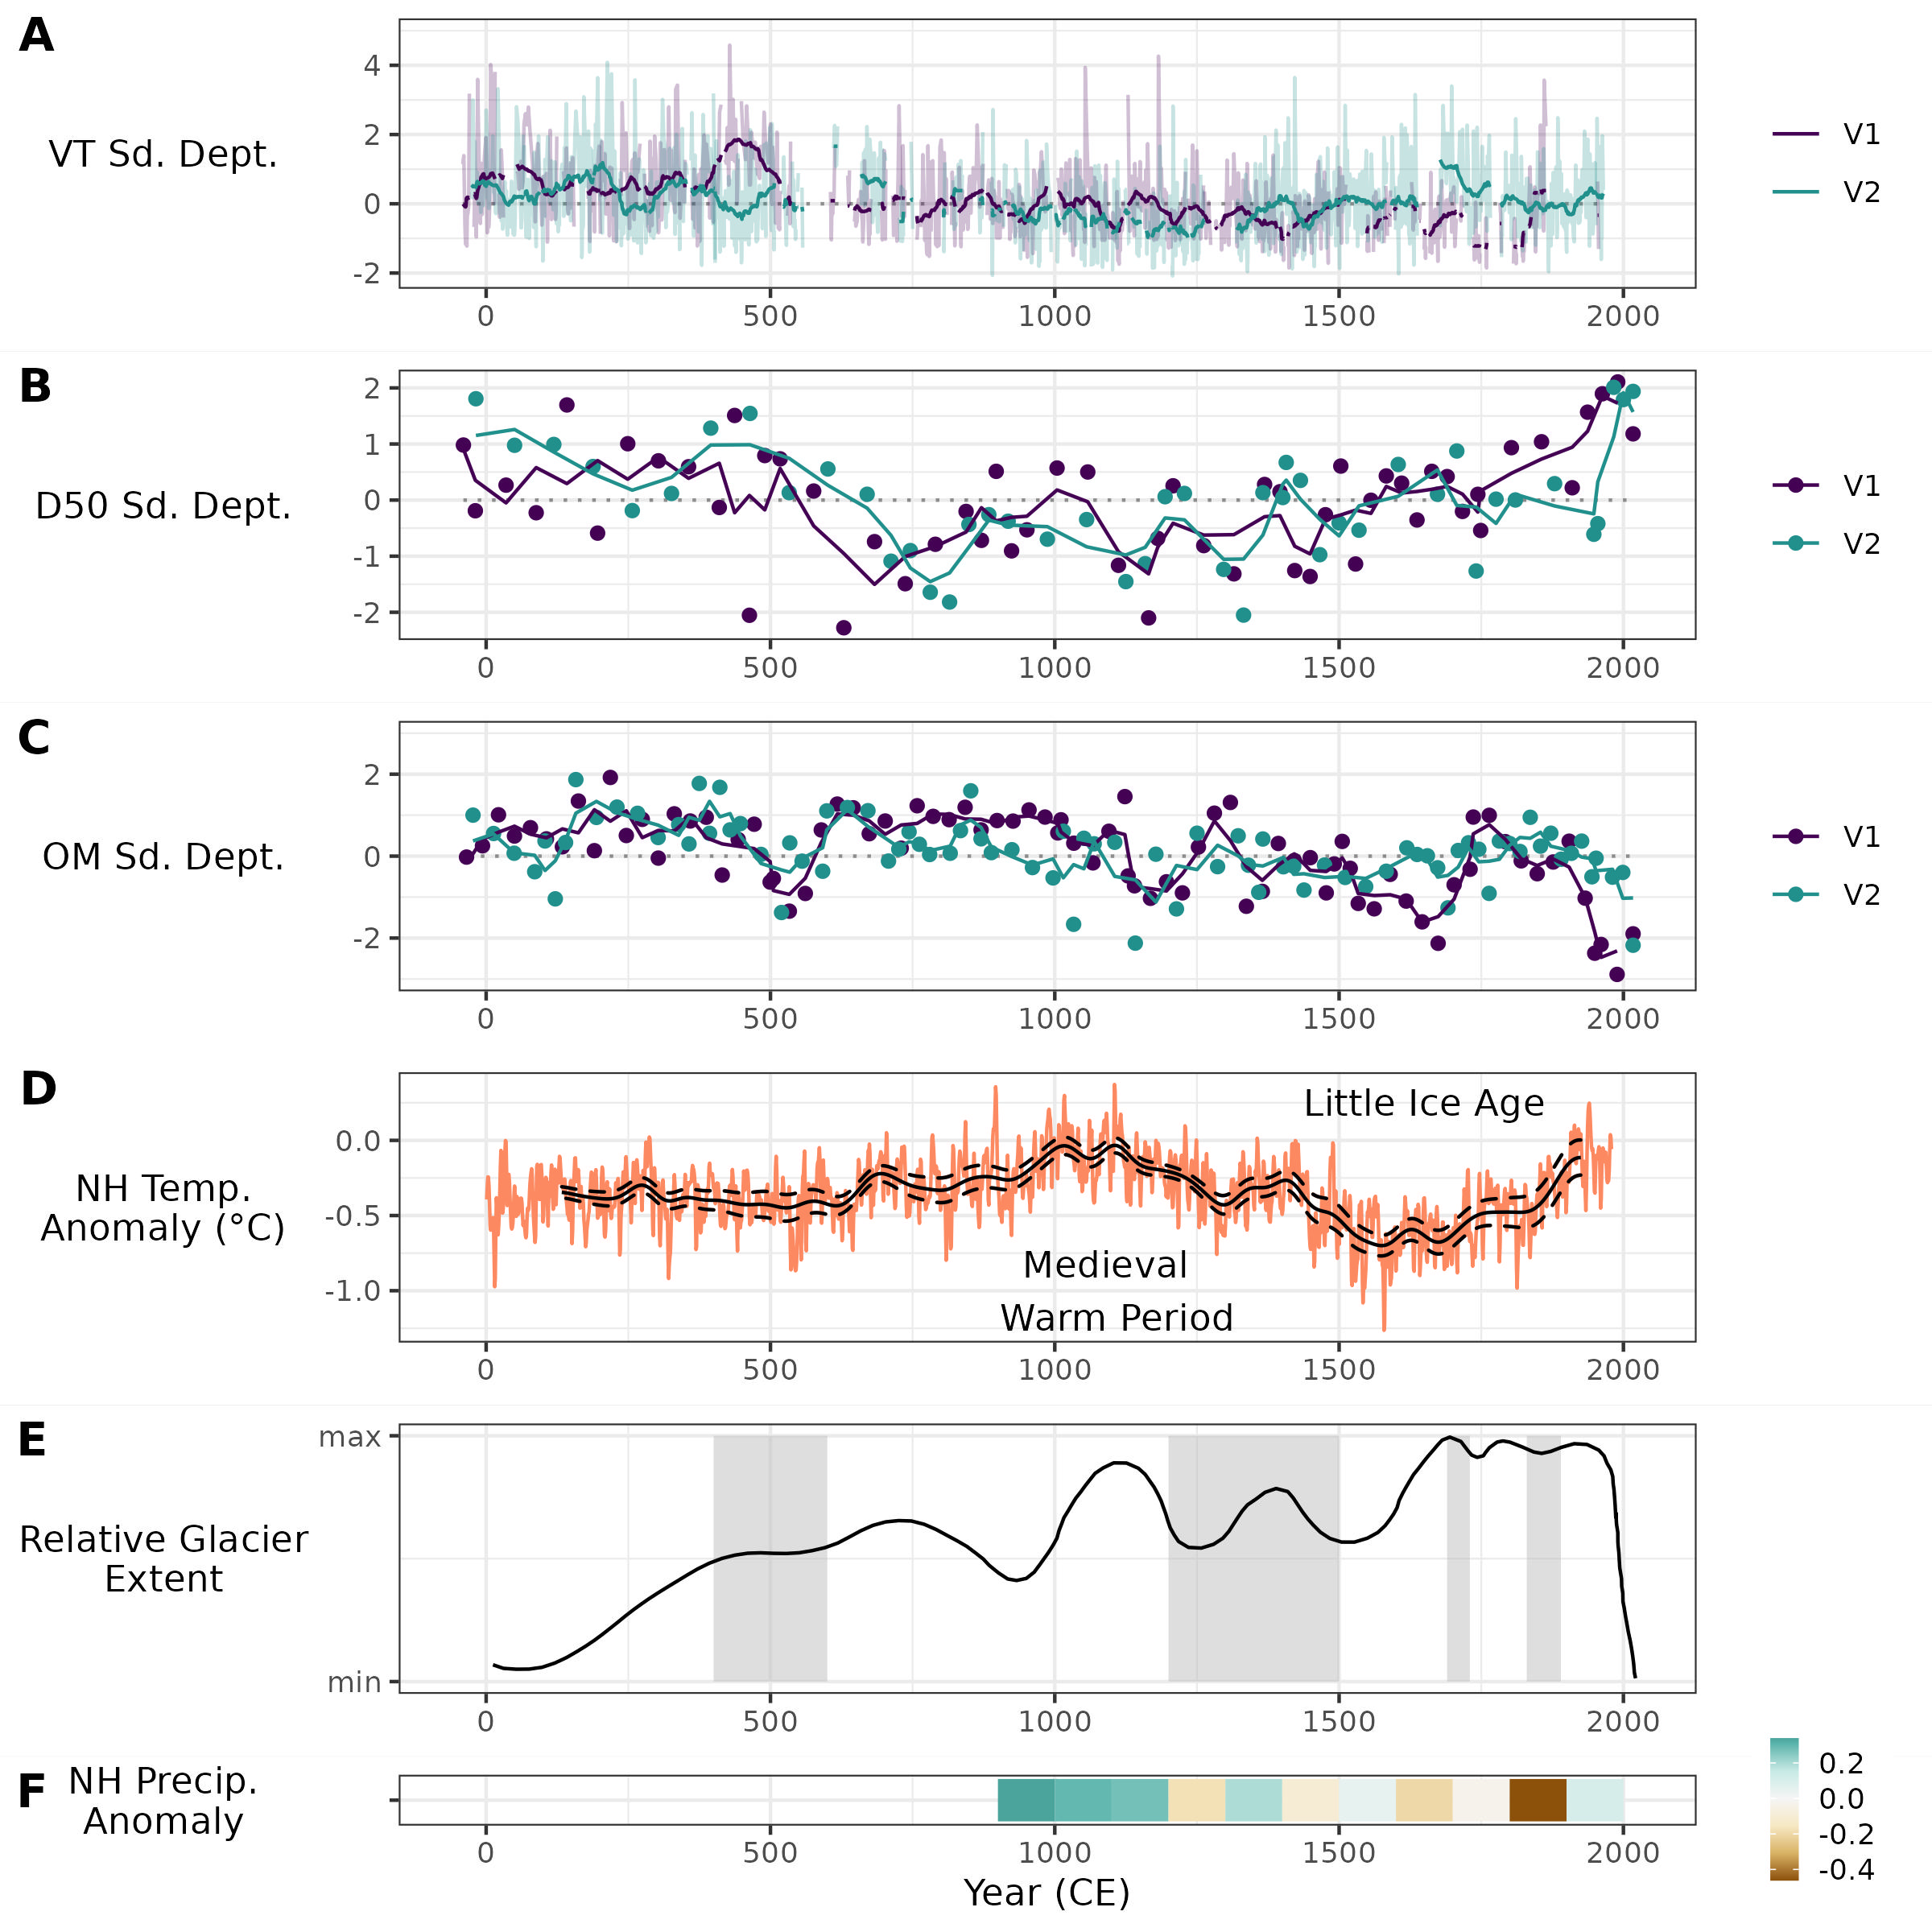
\includegraphics[width=1\linewidth]{figs/all_core_stats_2k_anomalies} 

}

\caption{Cariboo Lake sediment characteristics for cores V1 (purple) and V2 (green) and Northern Hemisphere (NH) climate proxies. A, is the standardized departure (Sd. Dept.) from the mean varve thickness (VT) for annual couplets (light colour) and 30-year moving average (dark lines). B, is the standardized departure from the mean percent organic matter (OM) for cores V1 and V2. The coloured dots represent percent OM at 2.5 - 5 cm intervals and the coloured lines are the 3 sample (~75 year) moving average. C, is the standardized departure from the mean D~50~ grain size, the coloured dots represent D~50~ grain size at 5 - 10 cm intervals and the coloured lines are the 3 sample (~125 year) moving average. D, Moberg et al. (2005) Nothern Hemisphere annual temperature anomaly from the 1961-1990 mean, the orange line is the full reconstruction from high and low frequency proxies, and the black line is the low frequency proxy component with upper and lower uncertainty marked by dashed blue lines. MCA is the Medieval Climatic Anomaly and LIA is the Little Ice Age. E, Solomina et al. (2016)  reconstructed relative glacier extent in western North America (black line), expansion of the Castle Creek glacier (blue bars, Maurer et al., 2012), and periods of peak glacier extent in western Canada (gray bars, Solomina et al., 2016). F, Ljungqvist et al. (2016) Nothern Hemisphere hydroclimate variability, expressed as standardized unitless anomalies ranging from -2 to 2, relative to the centennial mean and standard deviation over the eleventh-nineteenth centuries (see methods in Ljungqvist et al. 2016).}\label{fig:proxy-comparison}
\end{figure}

\hypertarget{conclusions}{%
\section{Conclusions}\label{conclusions}}

The moderated-sized Cariboo Lake provides a very good record of
deglacial and Holocene sediment inputs for central British Columbia. The
steep climatic gradient from the wetter, glacier covered, headwaters to
the semi-arid, lower elevation zones of the lake, result in sediment
input via the main Cariboo Lake delta that is predominately derived from
the glacier production zone. This conclusion is supported by the
down-lake trends observed in grain-size and organic matter content. The
smaller alluvial-fan deltas from side tributaries appear to be
paraglacial relic features, similar to those described in
\citet{Church1972}, and likely formed during deglaciation and the
earliest Holocene as no evidence of significant inputs during the
Holocene were found in this study.

\begin{enumerate}
\def\labelenumi{\arabic{enumi}.}
\tightlist
\item
  Sub-bottom acoustic records provide a coarse temporal resolution
  chronology of early and mid-Holocene sediment accumulation.
  \textbf{The transition from massive to acoustically well-layered
  sediments is estimated to have occurred around 10.5 to 9 ka BP. There
  is uncertainty with the timing of this transition as sediment
  accumulation rates have been extrapolated from the 2 ka old sediment
  cores.} Still, the 10.5 to 9 ka BP transition is similar to other
  glacier, lake and climate records across British Columbia and Alberta
  suggesting fairly consistent and rapid withdrawal of valley-bottom
  glacier ice into higher elevation zones.
\item
  \textbf{There were limitations in the ability to retrieve sufficiently
  long cores (\textgreater{} 10-15 m), that would provide a high
  resolution record of sediment inputs to Cariboo Lake over the entire
  Holocene.} If trends observed in other southern Canadian Cordilleran
  lakes prevail, the early and mid-Holocene input of sediment during the
  hypsithermal would have been significantly reduced resulting in a
  Holocene sediment package within the 10-15 m range. Acoustic Facies B
  most likely represents this unit.
\item
  Sedimentary structures in the long cores indicated sediment delivery,
  over the late Holocene to present, is dominated by similar fractions
  of silt (spring freshet) and clay (winter settling) resulting in the
  formation of rhythmically laminated couplets that are mainly varves.
  \textbf{The fraction of fine clastic sediments observed in the Cariboo
  Lake cores is high compared to other lakes in the Canadian Cordillera
  which typically have a larger fraction of coarse sediment from more
  frequent fall or spring high flows.} While there is relatively close
  agreement between sediment chronology from laminae counting and the
  two AMS dates, it is not possible to develop a chronology that
  provides a precisely dated high-resolution sediment yield record over
  the last 2 ka. However, the observed mean accumulation rate
  \textbf{(1.6 mm yr\textsuperscript{-1})}, the variance in accumulation
  rates and the low-frequency trends are important indicators of late
  Holocene environmental change.
\item
  \textbf{Periods of peak glacier extent, such as during the First
  Millennial Advance (\textasciitilde200 to 700 CE) and Little Ice Age
  (\textasciitilde1600 to 1900 CE) are best correlated with grain size
  in Cariboo Lake. The trends in varve thickness were not as strong but
  still help confirm trends observed in grain size. Organic matter
  content is the least correlated with the other sediment metrics and
  may be more sensitive to vegetation changes in the basin. We conclude
  that sediment accumulation in Cariboo Lake was more sensitive to
  glacier activity and sediment production during the LIA compared to
  earlier advances.}
\item
  The greatest deviation in varve thickness, grain size, and organic
  matter above normal occurs after 1860 CE and may be related to climate
  warming following the LIA. However, there are complications in this
  watershed via large-scale mining proximal to the lake and some upper
  watershed deforestation. These land-use and land-cover changes may
  have also been contributing factors to an increase in sediment
  delivery to the lake.
\item
  \textbf{Upstream filtering and storage of glacier eroded sediment may
  reduce the strength of the climate-sediment signal for Cariboo Lake.
  However, there is ample evidence that the sediment record spanning the
  last 2000 years gives better temporal resolution of watershed dynamics
  compared to other available records in the Interior Ranges of British
  Columbia. While the results presented here broadly agree with the
  primary glacier advances over the past 2000 years, further study of
  the laminated Cariboo Lake sediment record is required to better
  determine the exact timing and importance (i.e.~signal strength) of
  sediment inputs related to shifts of climate and glacier activity
  across of the south eastern Canadian Cordillera.}
\end{enumerate}

\pagebreak

\hypertarget{acknowledgements}{%
\section{Acknowledgements}\label{acknowledgements}}

We thank Michael Allchin, Laszlo Enyedy, and Caitlin Langford at the
Quesnel River Research Centre for assistance in field. Brian Menounos
kindly provided access to vibra-coring equipment. Mike Gorton, George
Kretschmann, Anna Soleski and Selina Amaral provided assistance with lab
analysis of sediment samples. Funding was provided by the University of
Toronto.

\pagebreak

\bibliographystyle{sageh}
\begin{thebibliography}{68}
\providecommand{\natexlab}[1]{#1}
\providecommand{\url}[1]{\texttt{#1}}
\providecommand{\urlprefix}{URL }
\expandafter\ifx\csname urlstyle\endcsname\relax
  \providecommand{\doi}[1]{DOI:\discretionary{}{}{}#1}\else
  \providecommand{\doi}{DOI:\discretionary{}{}{}\begingroup
  \urlstyle{rm}\Url}\fi

\bibitem[{Allen and Smith(2007)}]{Allen2007}
Allen SM and Smith DJ (2007) {Late Holocene glacial activity of Bridge Glacier,
  British Columbia Coast Mountains}.
\newblock \emph{Canadian Journal of Earth Sciences} 44(12): 1753--1773.
\newblock \doi{10.1139/E07-059}.

\bibitem[{Ballantyne(2002)}]{Ballantyne2002}
Ballantyne CK (2002) {Paraglacial geomorphology}.
\newblock \emph{Quaternary science reviews} 21(18): 1935--2017.

\bibitem[{Beedle et~al.(2015)Beedle, Menounos and Wheate}]{Beedle2015}
Beedle MJ, Menounos BP and Wheate R (2015) {Glacier change in the Cariboo
  Mountains, British Columbia, Canada (1952-2005)}.
\newblock \emph{Cryosphere} 9(1): 65--80.
\newblock \doi{10.5194/tc-9-65-2015}.

\bibitem[{Bolch and Bolch(2008)}]{Bolch2008}
Bolch Ts and Bolch Ta (2008) {GLIMS Glacier Database}.
\newblock \doi{10.7265/N5V98602}.

\bibitem[{Brown et~al.(2006)Brown, Fitton, Schoups, Allen, Wahl and
  Hebda}]{Brown2006}
Brown KJ, Fitton RJ, Schoups G, Allen GB, Wahl KA and Hebda RJ (2006) {Holocene
  precipitation in the coastal temperate rainforest complex of southern British
  Columbia, Canada}.
\newblock \emph{Quaternary Science Reviews} 25(21-22): 2762--2779.
\newblock \doi{10.1016/j.quascirev.2006.02.020}.

\bibitem[{Church and Ryder(1972)}]{Church1972}
Church M and Ryder JM (1972) {Paraglacial Sedimentation: A Consideration of
  Fluvial Processes Conditioned by Glaciation}.
\newblock \emph{GSA Bulletin} 83(10): 3059--3072.
\newblock \doi{10.1130/0016-7606(1972)83[3059:PSACOF]2.0.CO;2}.
\newblock
  \urlprefix\url{https://doi.org/10.1130/0016-7606(1972)83[3059:PSACOF]2.0.CO
  http://0.0.0.2}.

\bibitem[{Clague et~al.(2010)Clague, Koch and Geertsema}]{Clague2010}
Clague JJ, Koch J and Geertsema M (2010) {Expansion of outlet glaciers of the
  Juneau Icefield in northwest British Columbia during the past two millennia}.
\newblock \emph{The Holocene} 20(3): 447--461.
\newblock \doi{10.1177/0959683609353433}.
\newblock \urlprefix\url{https://doi.org/10.1177/0959683609353433}.

\bibitem[{Clague et~al.(1989)Clague, Mathews, Ryder, Hughes, Rutter, Jackson,
  Matthews and MacDonald}]{Clague1989}
Clague JJ, Mathews W, Ryder J, Hughes O, Rutter NW, Jackson L, Matthews J and
  MacDonald G (1989) {Quaternary geology of the Canadian Cordillera}.
\newblock In: \emph{Quaternary geology of Canada and Greenland}. North America:
  Geological Society of America, pp. 15--96.
\newblock \doi{10.1130/dnag-gna-k1.15}.
\newblock
  \urlprefix\url{https://pubs.geoscienceworld.org/books/book/853/chapter/4856715/}.

\bibitem[{Cockburn and Lamoureux(2008)}]{Cockburn2008}
Cockburn JM and Lamoureux SF (2008) {Inflow and lake controls on short-term
  mass accumulation and sedimentary particle size in a High Arctic lake:
  Implications for interpreting varved lacustrine sedimentary records}.
\newblock \emph{Journal of Paleolimnology} 40(3): 923--942.
\newblock \doi{10.1007/s10933-008-9207-5}.

\bibitem[{Crookshanks and Gilbert(2008)}]{Crookshanks2008}
Crookshanks S and Gilbert R (2008) {Continuous, diurnally fluctuating turbidity
  currents in Kluane Lake, Yukon Territory}.
\newblock \emph{Canadian journal of earth sciences} 45(10): 1123--1138.

\bibitem[{Desloges(1999)}]{Desloges1999}
Desloges JR (1999) {Geomorphic and climatic interpretations of abrupt changes
  in glaciolacustrine deposition at Moose Lake, British Columbia, Canada}.
\newblock \emph{Gff} 121(3): 202--207.
\newblock \doi{10.1080/11035899901213202}.

\bibitem[{Desloges and Gilbert(1994)}]{Desloges1994d}
Desloges JR and Gilbert R (1994) {Sediment source and hydroclimatic inferences
  from glacial lake sediments: the postglacial sedimentary record of Lillooet
  Lake, British Columbia}.
\newblock \emph{Journal of Hydrology} 159(1-4): 375--393.
\newblock \doi{10.1016/0022-1694(94)90268-2}.
\newblock
  \urlprefix\url{https://www.sciencedirect.com/science/article/pii/0022169494902682}.

\bibitem[{Dirszowsky and Desloges(1997)}]{Dirszowsky1997a}
Dirszowsky RW and Desloges JR (1997) {Glaciolacustrine sediments and neoglacial
  history of the Chephren lake basin, Banff National Park, Alberta}.
\newblock \emph{Geographie Physique Et Quaternaire} 51(1): 41--53.
\newblock \doi{10.7202/004804ar}.

\bibitem[{Filippelli et~al.(2006)Filippelli, Souch, Menounos, Slater-Atwater,
  {Timothy Jull} and Slaymaker}]{Filippelli2006}
Filippelli GM, Souch C, Menounos B, Slater-Atwater S, {Timothy Jull} AJ and
  Slaymaker O (2006) {Alpine lake sediment records of the impact of glaciation
  and climate change on the biogeochemical cycling of soil nutrients}.
\newblock \emph{Quaternary research} 66(1): 158--166.

\bibitem[{Gardner and Jones(1985)}]{Gardner1985}
Gardner JS and Jones NK (1985) {Evidence for a Neoglacial advance of the
  Boundary Glacier, Banff National Park, Alberta}.
\newblock \emph{Canadian Journal of Earth Sciences} 22(11): 1753--1755.
\newblock \doi{10.1139/e85-185}.
\newblock \urlprefix\url{https://doi.org/10.1139/e85-185}.

\bibitem[{Gilbert and Desloges(2012)}]{Gilbert2012}
Gilbert R and Desloges JR (2012) {Late glacial and Holocene sedimentary
  environments of Quesnel Lake, British Columbia}.
\newblock \emph{Geomorphology} 179: 186--196.
\newblock \doi{10.1016/j.geomorph.2012.08.010}.
\newblock \urlprefix\url{http://dx.doi.org/10.1016/j.geomorph.2012.08.010}.

\bibitem[{Gilbert et~al.(1997)Gilbert, Desloges and Clague}]{Gilbert1997}
Gilbert R, Desloges JR and Clague J (1997) {The glacilacustrine sedimentary
  environment of Bowser Lake in the northern Coast Mountains of British
  Columbia, Canada}.
\newblock \emph{Journal of Paleolimnology} 17(3): 333--348.
\newblock \doi{10.1023/A:1007900411724}.
\newblock \urlprefix\url{http://link.springer.com/10.1023/A:1007900411724}.

\bibitem[{Gray et~al.(2010)Gray, Pasternack and Watson}]{Gray2010}
Gray AB, Pasternack GB and Watson EB (2010) {Hydrogen peroxide treatment
  effects on the particle size distribution of alluvial and marsh sediments}.
\newblock \emph{The Holocene} 20(2): 293--301.
\newblock \doi{10.1177/0959683609350390}.
\newblock
  \urlprefix\url{http://journals.sagepub.com/doi/10.1177/0959683609350390}.

\bibitem[{Hallett et~al.(1997)Hallett, Hills and Clague}]{Hallett1997}
Hallett DU, Hills LV and Clague JJ (1997) {New accelerator mass spectrometry
  radiocarbon ages for the Mazama tephra layer from Kootenay National Park,
  British Columbia, Canada}.
\newblock \emph{Canadian Journal of Earth Sciences} 34(9): 1202--1209.
\newblock \doi{10.1139/e17-096}.

\bibitem[{Haslett and Parnell(2008)}]{Haslett2008}
Haslett J and Parnell A (2008) simple monotone process with application to
  radiocarbon-dated depth chronologies.
\newblock \emph{Applied statistics} 57(4): 399--418.

\bibitem[{Heideman et~al.(2018)Heideman, Menounos and Clague}]{Heideman2017}
Heideman M, Menounos B and Clague JJ (2018) {A multi-century estimate of
  suspended sediment yield from Lillooet Lake, southern Coast Mountains,
  Canada}.
\newblock \emph{Canadian journal of earth sciences} 55(1): 18--32.

\bibitem[{Heideman et~al.(2015)Heideman, Menounos and Clague}]{Heideman2015}
Heideman M, Menounos BP and Clague J (2015) {An 825-year long varve record from
  Lillooet Lake, British Columbia, and its potential as a flood proxy}.
\newblock \emph{Quaternary Science Reviews} 126: 158--174.
\newblock \doi{10.1016/j.quascirev.2015.08.017}.
\newblock \urlprefix\url{http://dx.doi.org/10.1016/j.quascirev.2015.08.017}.

\bibitem[{Hodder et~al.(2006)Hodder, Desloges and Gilbert}]{Hodder2006b}
Hodder KR, Desloges JR and Gilbert R (2006) {Pattern and timing of sediment
  infill at glacier-fed Mud Lake: Implications for lateglacial and Holocene
  environments in the Monashee Mountain region of British Columbia, Canada}.
\newblock \emph{Holocene} 16(5): 705--716.
\newblock \doi{10.1191/0959683606hl965rp}.

\bibitem[{Hodder et~al.(2007)Hodder, Gilbert and Desloges}]{Hodder2007c}
Hodder KR, Gilbert R and Desloges JR (2007) {Glaciolacustrine varved sediment
  as an alpine hydroclimatic proxy}.
\newblock \emph{Journal of Paleolimnology} 38(3): 365--394.
\newblock \doi{10.1007/s10933-006-9083-9}.

\bibitem[{Huber and Knutti(2012)}]{Huber2012}
Huber M and Knutti R (2012) {Anthropogenic and natural warming inferred from
  changes in Earth's energy balance}.
\newblock \emph{Nature geoscience} 5(1): 31--36.

\bibitem[{Jerolmack and Paola(2010)}]{Jerolmack2010}
Jerolmack DJ and Paola C (2010) {Shredding of environmental signals by sediment
  transport}.
\newblock \emph{Geophysical research letters} 37(19): n/a.

\bibitem[{Koch et~al.(2007)Koch, Osborn and Clague}]{Koch2007a}
Koch J, Osborn GD and Clague JJ (2007) {Pre-'Little Ice Age' glacier
  fluctuations in Garibaldi Provincial Park, Coast Mountains, British Columbia,
  Canada}.
\newblock \emph{Holocene} 17(8): 1069--1078.
\newblock \doi{10.1177/0959683607082546}.

\bibitem[{Leonard(1986)}]{Leonard1986}
Leonard EM (1986) {Use of lacustrine sedimentary sequences as indicators of
  Holocene glacial history, Banff National Park, Alberta, Canada}.
\newblock \emph{Quaternary Research} 26(2): 218--231.
\newblock \doi{10.1016/0033-5894(86)90106-7}.

\bibitem[{Leonard(1997)}]{Leonard1997}
Leonard EM (1997) {The relationship between glacial activity and sediment
  production: Evidence from a 4450-year varve record of neoglacial
  sedimentation in Hector Lake, Alberta, Canada}.
\newblock \emph{Journal of Paleolimnology} 17(3): 319--330.

\bibitem[{Leonard and Reasoner(1999)}]{Leonard1999}
Leonard EM and Reasoner MA (1999) {A continuous holocene glacial record
  inferred from proglacial lake sediments in Banff National Park, Alberta,
  Canada}.
\newblock \emph{Quaternary Research} 51(1): 1--13.
\newblock \doi{10.1006/qres.1998.2009}.
\newblock
  \urlprefix\url{https://www.sciencedirect.com/science/article/pii/S0033589498920099}.

\bibitem[{Ljungqvist et~al.(2016)Ljungqvist, Krusic, Sundqvist, Zorita,
  Brattstrom and Frank}]{Ljungqvist2016}
Ljungqvist FC, Krusic PJ, Sundqvist HS, Zorita E, Brattstrom G and Frank D
  (2016) {Northern hemisphere hydroclimate variability over the past twelve
  centuries}.
\newblock \emph{Nature} 532: 94+.
\newblock
  \urlprefix\url{https://link.gale.com/apps/doc/A449108229/EAIM?u=usaskmain&sid=bookmark-EAIM&xid=1dfbd232}.

\bibitem[{Lowe et~al.(1997)Lowe, Green, Northcote and Hall}]{Lowe1997}
Lowe DJ, Green JD, Northcote TG and Hall KJ (1997) {Holocene Fluctuations of a
  Meromictic Lake in Southern British Columbia}.
\newblock \emph{Quaternary research} 48(1): 100--113.

\bibitem[{Luckman(1986)}]{Luckman1986}
Luckman BH (1986) {Reconstruction of Little Ice Age Events in the Canadian
  Rocky Mountains}.
\newblock \emph{G{\'{e}}ographie physique et quaternaire} 40(1): 17--28.

\bibitem[{Luckman(1988)}]{Luckman1988}
Luckman BH (1988) {8000 year old wood from the Athabasca Glacier, Alberta}.
\newblock \emph{Canadian Journal of Earth Sciences} 25(1): 148--151.
\newblock \doi{10.1139/e88-015}.
\newblock \urlprefix\url{http://www.nrcresearchpress.com/doi/10.1139/e88-015}.

\bibitem[{Luckman(1993)}]{Luckman1993}
Luckman BH (1993) {Glacier fluctuation and tree-ring records for the last
  millennium in the Canadian Rockies}.
\newblock \emph{Quaternary Science Reviews} 12(6): 441--450.
\newblock \doi{10.1016/S0277-3791(05)80008-3}.

\bibitem[{Luckman(1995)}]{Luckman1995}
Luckman BH (1995) {Calendar-dated, early ‘Little Ice Age' glacier advance at
  Robson Glacier, British Columbia, Canada}.
\newblock \emph{The Holocene} 5(2): 149--159.
\newblock \doi{10.1177/095968369500500203}.

\bibitem[{Luckman(2000)}]{Luckman2000g}
Luckman BH (2000) {The Little Ice Age in the Canadian Rockies}.
\newblock \emph{Geomorphology} 32(3-4): 357--384.
\newblock \doi{10.1016/S0169-555X(99)00104-X}.
\newblock
  \urlprefix\url{http://linkinghub.elsevier.com/retrieve/pii/S0169555X9900104X%5Cnfile:///Users/whobbs/Documents/PDFs/Papers2/Luckman/2000/Geomorphology
  2000
  Luckman.pdf%5Cnpapers2://publication/uuid/7AE71933-5443-41E0-B7B7-88A14B3C077A}.

\bibitem[{Luckman and Kavanagh(2000)}]{Luckman2000e}
Luckman BH and Kavanagh T (2000) {Impact of climate fluctuations on mountain
  environments in the Canadian Rockies}.
\newblock \emph{Ambio} 29(7): 371--380.
\newblock \doi{10.1639/0044-7447(2000)029[0371:IOCFOM]2.0.CO;2}.

\bibitem[{Luckman et~al.(1999)Luckman, Kavanagh, Craig and {St.
  George}}]{Luckman1999}
Luckman BH, Kavanagh TA, Craig I and {St George} RS (1999) {Earliest photograph
  of Athabasca and Dome Glaciers, Alberta}.
\newblock \emph{G{\'{e}}ographie physique et Quaternaire} 53(3): 401.
\newblock \doi{10.7202/004844ar}.
\newblock \urlprefix\url{http://id.erudit.org/iderudit/004844ar}.

\bibitem[{Masson-Delmotte et~al.(2013)Masson-Delmotte, Schulz, Abe-Ouchi, Beer,
  Ganopolski, {Gonz{\'{a}}lez Rouco}, Jansen, Lambeck, Luterbacher, Naish,
  Osborn, Otto-Bliesner, Quinn, Ramesh, Rojas, Shao and
  Timmermann}]{Masson2013}
Masson-Delmotte V, Schulz M, Abe-Ouchi A, Beer J, Ganopolski J, {Gonz{\'{a}}lez
  Rouco} JF, Jansen E, Lambeck K, Luterbacher J, Naish T, Osborn T,
  Otto-Bliesner B, Quinn T, Ramesh R, Rojas M, Shao X and Timmermann A (2013)
  \emph{{Information from paleoclimate archives}}.
\newblock Cambridge, UK: Cambridge University Press, pp. 383--464.
\newblock \doi{10.1017/CBO9781107415324.013}.

\bibitem[{Maurer et~al.(2012)Maurer, Menounos, Luckman, Osborn, Clague, Beedle,
  Smith and Atkinson}]{Maurer2012b}
Maurer MK, Menounos BP, Luckman BH, Osborn GD, Clague J, Beedle MJ, Smith R and
  Atkinson N (2012) {Late Holocene glacier expansion in the Cariboo and
  northern Rocky Mountains, British Columbia, Canada}.
\newblock \emph{Quaternary Science Reviews} 51: 71--80.
\newblock \doi{10.1016/j.quascirev.2012.07.023}.
\newblock
  \urlprefix\url{https://www.sciencedirect.com/science/article/pii/S0277379112002909
  http://resolver.scholarsportal.info/resolve/02773791/v51inone_c/71_lhgeitnrmbcc}.

\bibitem[{Menounos and Clague(2008)}]{Menounos2008c}
Menounos BP and Clague JJJ (2008) {Reconstructing hydro-climatic events and
  glacier fluctuations over the past millennium from annually laminated
  sediments of Cheakamus Lake, southern Coast Mountains, British Columbia,
  Canada}.
\newblock \emph{Quaternary Science Reviews} 27(7-8): 701--713.
\newblock \doi{10.1016/j.quascirev.2008.01.007}.

\bibitem[{Menounos et~al.(2004)Menounos, Koch, Osborn, Clague and
  Mazzucchi}]{Menounos2004}
Menounos BP, Koch J, Osborn GD, Clague J and Mazzucchi D (2004) {Early Holocene
  glacier advance, southern Coast Mountains, British Columbia, Canada}.
\newblock \emph{Quaternary Science Reviews} 23(14-15): 1543--1550.
\newblock \doi{10.1016/j.quascirev.2003.12.023}.
\newblock
  \urlprefix\url{https://www.sciencedirect.com/science/article/pii/S027737910400023X}.

\bibitem[{Menounos et~al.(2009)Menounos, Osborn, Clague and
  Luckman}]{Menounos2009b}
Menounos BP, Osborn GD, Clague J and Luckman BH (2009) {Latest Pleistocene and
  Holocene glacier fluctuations in western Canada}.
\newblock \emph{Quaternary Science Reviews} 28(21-22): 2049--2074.
\newblock \doi{10.1016/j.quascirev.2008.10.018}.

\bibitem[{Menounos et~al.(2006)Menounos, Schiefer and
  Slaymaker}]{Menounos2006b}
Menounos BP, Schiefer E and Slaymaker O (2006) {Nested temporal suspended
  sediment yields, Green Lake Basin, British Columbia, Canada}.
\newblock \emph{Geomorphology} 79(1-2): 114--129.
\newblock \doi{10.1016/j.geomorph.2005.09.020}.

\bibitem[{Moberg et~al.(2005)Moberg, Sonechkin, Holmgren, Datsenko and
  Karl{\'{e}}n}]{Moberg2005}
Moberg A, Sonechkin DM, Holmgren K, Datsenko MH and Karl{\'{e}}n W (2005)
  {Highly variable Northern Hemisphere temperatures reconstructed from low- and
  high-resolution proxy data}.
\newblock \emph{Nature} 433(7026): 613--617.
\newblock \doi{10.1038/nature03265}.

\bibitem[{Nelson et~al.(2016)Nelson, Ingram, Dugmore, Streeter, Peeples,
  McGovern, Hegmon, Arneborg, Kintigh, Brewington, Spielmann, Simpson,
  Strawhacker, Comeau, Torvinen, Madsen, Hambrecht and Smiarowski}]{Nelson2016}
Nelson MC, Ingram SE, Dugmore AJ, Streeter R, Peeples MA, McGovern TH, Hegmon
  M, Arneborg J, Kintigh KW, Brewington S, Spielmann KA, Simpson IA,
  Strawhacker C, Comeau LEL, Torvinen A, Madsen CK, Hambrecht G and Smiarowski
  K (2016) {Climate challenges, vulnerabilities, and food security}.
\newblock \emph{Proceedings of the National Academy of Sciences} 113(2):
  298--303.
\newblock \doi{10.1073/pnas.1506494113}.
\newblock \urlprefix\url{https://www.pnas.org/doi/abs/10.1073/pnas.1506494113}.

\bibitem[{Neukom et~al.(2019)Neukom, Barboza, Erb, Shi, Emile-Geay, Evans,
  Franke, Kaufman, L{\"{u}}cke, Rehfeld, Schurer, Zhu, Br{\"{o}}nnimann, Hakim,
  Henley, Ljungqvist, McKay, Valler, von Gunten, Lucke, Rehfeld, Schurer, Zhu,
  Bronnimann, Hakim, Henley, Ljungqvist, McKay, Valler and von
  Gunten}]{Neukom2019}
Neukom R, Barboza LA, Erb MP, Shi F, Emile-Geay J, Evans MN, Franke JJ, Kaufman
  DS, L{\"{u}}cke L, Rehfeld K, Schurer A, Zhu F, Br{\"{o}}nnimann S, Hakim GJ,
  Henley BJ, Ljungqvist FC, McKay N, Valler V, von Gunten L, Lucke L, Rehfeld
  K, Schurer A, Zhu F, Bronnimann S, Hakim GJ, Henley BJ, Ljungqvist FC, McKay
  N, Valler V and von Gunten L (2019) {Consistent multidecadal variability in
  global temperature reconstructions and simulations over the Common Era}.
\newblock \emph{Nature geoscience} 12(8): 643--649.
\newblock \doi{10.1038/s41561-019-0400-0}.

\bibitem[{Osborn et~al.(2007)Osborn, Menounos, Koch, Clague and
  Vallis}]{Osborn2007}
Osborn GD, Menounos BP, Koch J, Clague J and Vallis V (2007) {Multi-proxy
  record of Holocene glacial history of the Spearhead and Fitzsimmons ranges,
  southern Coast Mountains, British Columbia}.
\newblock \emph{Quaternary Science Reviews} 26(3-4): 479--493.
\newblock \doi{10.1016/j.quascirev.2006.09.003}.

\bibitem[{Osborn et~al.(2001)Osborn, Robinson and Luckman}]{Osborn2001}
Osborn GD, Robinson BJ and Luckman BH (2001) {Holocene and latest Pleistocene
  fluctuations of Stutfield Glacier, Canadian Rockies}.
\newblock \emph{Canadian Journal of Earth Sciences} 38(8): 1141--1155.
\newblock \doi{10.1139/e01-012}.

\bibitem[{Parnell et~al.(2011)Parnell, Buck and Doan}]{Parnell2011}
Parnell AC, Buck CE and Doan TK (2011) {A review of statistical chronology
  models for high-resolution, proxy-based Holocene palaeoenvironmental
  reconstruction}.
\newblock \emph{Quaternary science reviews} 30(21): 2948--2960.

\bibitem[{Parnell et~al.(2008)Parnell, Haslett, Allen, Buck and
  Huntley}]{Parnell2008}
Parnell AC, Haslett J, Allen JRM, Buck CE and Huntley B (2008) {A flexible
  approach to assessing synchroneity of past events using Bayesian
  reconstructions of sedimentation history}.
\newblock \emph{Quaternary science reviews} 27(19): 1872--1885.

\bibitem[{Reimer et~al.(2013)Reimer, Bard, Bayliss, Beck, Blackwell, {Bronk
  Ramsey}, Buck, Cheng, Edwards, Frieich, Grootes, Guilderson, Haflidason,
  Hajdas, Hatt{\'{e}}, Heaton, Hoffmann, Hogg, Hughen, Kaiser, Kromer, Manning,
  Niu, Reimer, Richards, Scott, Southon, Staff, Turney and van~der
  Plicht}]{Reimer2013}
Reimer PJ, Bard E, Bayliss A, Beck JW, Blackwell PG, {Bronk Ramsey} C, Buck CE,
  Cheng H, Edwards RL, Frieich M, Grootes PM, Guilderson TP, Haflidason H,
  Hajdas I, Hatt{\'{e}} C, Heaton TJ, Hoffmann DL, Hogg AG, Hughen KA, Kaiser
  KF, Kromer B, Manning SW, Niu M, Reimer RW, Richards DA, Scott EM, Southon
  JR, Staff RA, Turney CSM and van~der Plicht J (2013) {IntCal13 and Marine13
  Radiocarbon Age Calibration Curves 0–50,000 Years cal BP}.
\newblock \emph{Radiocarbon} 55(4): 1869--1887.

\bibitem[{Reyes et~al.(2006)Reyes, Wiles, Smith, Barclay, {Allen Scott Jackson
  Sonya Larocque Sarah Laxton Dave Lewis}, Calkin and Clague}]{Reyes2006}
Reyes ADV, Wiles GC, Smith DJ, Barclay DJ, {Allen Scott Jackson Sonya Larocque
  Sarah Laxton Dave Lewis} S, Calkin PE and Clague J (2006) {Expansion of
  alpine glaciers in Pacific North America in the first millennium A}.
\newblock \emph{Geology} 341(3).
\newblock \doi{10.1130/G21902.1}.
\newblock \urlprefix\url{https://www.sfu.ca/$\sim$qgrc/papers/1st millennium AD
  advance.pdf}.

\bibitem[{Ryder and Thomson(1986)}]{Ryder1986}
Ryder JM and Thomson B (1986) {Neoglaciation in the southern Coast Mountains of
  British Columbia: chronology prior to the late Neoglacial maximum}.
\newblock \emph{Canadian Journal of Earth Sciences} 23(3): 273--287.
\newblock \doi{10.1139/e86-031}.
\newblock \urlprefix\url{http://www.nrcresearchpress.com/doi/10.1139/e86-031}.

\bibitem[{Sabatier et~al.(2022)Sabatier, Moernaut, Bertrand, Daele, Kremer,
  Chaumillon, Arnaud, {Van Daele}, Kremer, Chaumillon and
  Arnaud}]{sabatier2022}
Sabatier P, Moernaut J, Bertrand S, Daele MV, Kremer K, Chaumillon E, Arnaud F,
  {Van Daele} M, Kremer K, Chaumillon E and Arnaud F (2022) {A Review of Event
  Deposits in Lake Sediments}.
\newblock \emph{Quaternary} 5(3): 34.
\newblock \doi{10.3390/quat5030034}.

\bibitem[{Schneider et~al.(2012)Schneider, Rasband and
  Eliceiri}]{Schneider2012}
Schneider CA, Rasband WS and Eliceiri KW (2012) {NIH Image to ImageJ: 25 years
  of image analysis}.
\newblock \emph{Nature Methods} 9(7): 671--675.
\newblock \doi{10.1038/nmeth.2089}.
\newblock \urlprefix\url{https://doi.org/10.1038/nmeth.2089}.

\bibitem[{Smith(2003)}]{Smith2003}
Smith JG (2003) {Aspects of the loss‐on‐ignition (loi) technique in the
  context of clay‐rich, glaciolacustrine sediments}.
\newblock \emph{Geografiska Annaler: Series A, Physical Geography} 85(1):
  91--97.
\newblock \doi{10.1111/1468-0459.00191}.
\newblock
  \urlprefix\url{https://www.tandfonline.com/doi/full/10.1111/1468-0459.00191}.

\bibitem[{Solomina et~al.(2016)Solomina, Bradley, Jomelli, Geirsdottir,
  Kaufman, Koch, McKay, Masiokas, Miller, Nesje, Nicolussi, Owen, Putnam,
  Wanner, Wiles and Yang}]{Solomina2016}
Solomina ON, Bradley RS, Jomelli V, Geirsdottir A, Kaufman DS, Koch J, McKay
  NP, Masiokas M, Miller G, Nesje A, Nicolussi K, Owen LA, Putnam AE, Wanner H,
  Wiles G and Yang B (2016) {Glacier fluctuations during the past 2000 years}.
\newblock \emph{Quaternary Science Reviews} 149: 61--90.
\newblock \doi{10.1016/j.quascirev.2016.04.008}.

\bibitem[{Steinman et~al.(2012)Steinman, Abbott, Mann, Stansell and
  Finney}]{Steinman2012}
Steinman BA, Abbott MB, Mann ME, Stansell ND and Finney BP (2012) \emph{{1,500
  year quantitative reconstruction of winter precipitation in the Pacific
  Northwest}}, volume 109.
\newblock National Academy of Sciences.
\newblock ISBN 1201083109.
\newblock \doi{10.1073/pnas.1201083109}.
\newblock \urlprefix\url{http://www.pnas.org/cgi/doi/10.1073/pnas.1201083109}.

\bibitem[{Steinman et~al.(2019)Steinman, Nelson, Abbott, Stansell, Finkenbinder
  and Finney}]{Steinman2019}
Steinman BA, Nelson DB, Abbott MB, Stansell ND, Finkenbinder MS and Finney BP
  (2019) {Lake sediment records of Holocene hydroclimate and impacts of the
  Mount Mazama eruption, north-central Washington, USA}.
\newblock \emph{Quaternary Science Reviews} 204: 17--36.
\newblock \doi{10.1016/j.quascirev.2018.09.018}.
\newblock \urlprefix\url{https://doi.org/10.1016/j.quascirev.2018.09.018}.

\bibitem[{Turney et~al.(2019)Turney, McGregor, Francus, Abram, Evans, Goosse,
  {Von Gunten}, Kaufman, Linderholm, Loutre and Neukom}]{Turney2019}
Turney CSM, McGregor HV, Francus P, Abram N, Evans MN, Goosse H, {Von Gunten}
  L, Kaufman D, Linderholm H, Loutre MF and Neukom R (2019) {Introduction to
  the special issue "climate of the past 2000 years: Regional and
  trans-regional syntheses"}.
\newblock \emph{Climate of the past} 15(2): 611--615.

\bibitem[{Westgate(1977)}]{Westgate1977}
Westgate JA (1977) {Identification and Significance of Late Holocene Tephra
  From Otter Creek, Southern British Columbia, and Localities in West-Central
  Alberta.}
\newblock \emph{Can J Earth Sci} 14(11): 2593--2600.
\newblock \doi{10.1139/e77-224}.

\bibitem[{Wohl et~al.(2019)Wohl, Brierley, Cadol, Coulthard, Covino, Fryirs,
  Grant, Hilton, Lane, Magilligan, Meitzen, Passalacqua, Poeppl, Rathburn and
  Sklar}]{Wohl2019}
Wohl E, Brierley G, Cadol D, Coulthard TJ, Covino T, Fryirs KA, Grant G, Hilton
  RG, Lane SN, Magilligan FJ, Meitzen KM, Passalacqua P, Poeppl RE, Rathburn SL
  and Sklar LS (2019) {Connectivity as an emergent property of geomorphic
  systems}.
\newblock \emph{Earth Surface Processes and Landforms} 44(1): 4--26.
\newblock \doi{10.1002/esp.4434}.

\bibitem[{Wood and Smith(2004)}]{Wood2004}
Wood C and Smith DJ (2004) {Dendroglaciological Evidence For A Neoglacial
  Advance Of the Saskatchewan Glacier, Banff National Park, Canadian Rocky
  Mountains}.
\newblock \emph{Tree-Ring Research} 60(1): 59--65.
\newblock \doi{10.3959/1536-1098-60.1.59}.

\bibitem[{Zdanowicz et~al.(1999)Zdanowicz, Zielinski and
  Germani}]{Zdanowicz1999}
Zdanowicz CM, Zielinski GA and Germani MS (1999) {Mount Mazama eruption:
  Calendrical age verified and atmospheric impact assessed}.
\newblock \emph{Geology} 27(7): 621--624.
\newblock \doi{10.1130/0091-7613(1999)027<0621:MMECAV>2.3.CO;2}.

\bibitem[{Zolitschka(1991)}]{Zolitschka1991}
Zolitschka B (1991) {Absolute dating of late quaternary lacustrine sediments by
  high resolution varve chronology}.
\newblock \emph{Hydrobiologia} 214(1): 59--61.

\bibitem[{Zolitschka et~al.(2015)Zolitschka, Francus, Ojala and
  Schimmelmann}]{Zolitschka2015a}
Zolitschka B, Francus P, Ojala AE and Schimmelmann A (2015) {Varves in lake
  sediments - a review}.
\newblock \emph{Quaternary Science Reviews} 117: 1--41.
\newblock \doi{10.1016/j.quascirev.2015.03.019}.
\newblock \urlprefix\url{http://dx.doi.org/10.1016/j.quascirev.2015.03.019}.

\end{thebibliography}

\end{document}
